% main.tex
\documentclass[12pt, a4paper]{article}
\usepackage{svg}
% Gọi file cài đặt
% setup/packages.tex
\usepackage[utf8]{vietnam}
\usepackage[left=3.5cm,right=2.5cm,top=2cm,bottom=2cm]{geometry}
\setlength{\parindent}{1cm}
\usepackage{indentfirst}
\usepackage{graphicx}
\usepackage{changepage}
\usepackage{hyperref}
\usepackage{titlesec}
\usepackage{float}
\usepackage{array}
\usepackage{ragged2e}
\usepackage[justification=centering]{caption}
\usepackage{array}
\usepackage{tabu}
\usepackage{tabularx}
\usepackage{longtable}
\newcolumntype{P}[1]{>{\RaggedRight\arraybackslash}p{#1}}
\newcolumntype{Y}{>{\RaggedRight\arraybackslash}X}
\usepackage{multirow}
\usepackage{multicol}
\usepackage{float}
\usepackage[table]{xcolor}
\usepackage{listings}
\usepackage{amsmath, amssymb, amsthm}
\usepackage{tikz}
\usetikzlibrary{arrows.meta,positioning,calc,fit}
\usepackage{scrextend}
\usepackage{fancybox}
\usepackage{fancyhdr}
\usepackage{enumitem}
\usepackage{tcolorbox}
% Cấu hình Listings
\lstdefinelanguage{Verilog}{
  keywords={module, endmodule, input, output, wire, reg, always, posedge, negedge, begin, end, if, else, case, endcase, default, assign, initial, parameter},
  sensitive=true,
  morecomment=[l]{//},
  morecomment=[s]{/*}{*/},
  morestring=[b]"
}

\lstset{
    language=Verilog,
    frame=single,
    backgroundcolor=\color{lightgray},
    basicstyle=\ttfamily\small,
    keywordstyle=\color{blue}\bfseries,
    commentstyle=\color{green!60!black},
    stringstyle=\color{red},
    numberstyle=\tiny\color{black},
    numbers=left,
    numbersep=6pt,
    tabsize=4,
    breaklines=true,
    captionpos=b
}

% Cập nhật Header
\pagestyle{fancy}
\fancyhf{}
\lhead{Cơ sở dữ liệu}
\rhead{Nhóm 38}
\rfoot{Trang \thepage}
\renewcommand{\headrulewidth}{1pt}
\renewcommand{\footrulewidth}{1pt}


% Giữ bố cục mẫu; đủ chiều cao cho header tiếng Việt.
\setlength{\headheight}{15pt}
\addtolength{\topmargin}{-3pt}
\renewcommand{\refname}{Tài liệu tham khảo}

% Bổ sung cho báo cáo CSDL: kiểu hiển thị mã SQL (giữ nguyên khung, nền, cỡ chữ của mẫu)
% sqllisting.tex -- kiểu listing cho mã SQL (PostgreSQL, PL/pgSQL) có chú thích và chuỗi tiếng Việt.
% Kế thừa khung, nền, đánh số dòng từ \lstset của mẫu; chỉ đổi ngôn ngữ và bổ sung ánh xạ ký tự.
\lstdefinestyle{sqlvn}{
  language=SQL,
  morekeywords={BIGINT, VARCHAR, TEXT, DATE, TIMESTAMPTZ, INT, GENERATED, IDENTITY, CONSTRAINT, REFERENCES,
    UNIQUE, CHECK, DEFAULT, CURRENT_TIMESTAMP, INTERSECT, EXISTS, FILTER, INTERVAL, EXTRACT, MONTH,
    EXCLUDE, USING, GIST, EXTENSION, IF, ROLE, LOGIN, NOSUPERUSER, NOCREATEDB, NOCREATEROLE, GRANT, REVOKE,
    USAGE, SCHEMA, ALL, TABLES, SEQUENCES, PUBLIC, SET, RESET, ALTER, ADD, FUNCTION, RETURNS, RETURN,
    QUERY, EXECUTE, LANGUAGE, STABLE, BEGIN, END, LIMIT, MAX, COUNT, LEFT, JOIN, ON, AS, IS, NULL, VIEW, WITH},
  sensitive=false,
  morecomment=[l]{--},
  morestring=[b]',
  extendedchars=true,
  showstringspaces=false,
  basicstyle=\ttfamily\footnotesize,
  % In A4: footnotesize của lớp 12pt là 10pt. Dùng cột "fullflexible" + keepspaces để chữ
  % đơn cách tự nhiên (không giãn ký tự), ít dòng bị gãy hơn mà vẫn giữ thẳng hàng.
  columns=fullflexible,
  keepspaces=true,
  upquote=true,
  numberstyle=\scriptsize\color{black},
  breakindent=2em,
  breakatwhitespace=true,
  literate=
    {Á}{{\'A}}1 {Ú}{{\'U}}1 {à}{{\`a}}1 {á}{{\'a}}1 {â}{{\^a}}1 {é}{{\'e}}1 {ê}{{\^e}}1 {ì}{{\`\i}}1
    {ò}{{\`o}}1 {ó}{{\'o}}1 {ô}{{\^o}}1 {ù}{{\`u}}1 {ú}{{\'u}}1 {Đ}{{\DJ}}1 {đ}{{\dj}}1 {ư}{{\uhorn}}1
    {ạ}{{\d a}}1 {ả}{{\h a}}1 {ậ}{{\d\acircumflex}}1 {Ế}{{\'\ECIRCUMFLEX}}1 {ề}{{\`\ecircumflex}}1 {ệ}{{\d\ecircumflex}}1 {ỉ}{{\h i}}1 {ị}{{\d i}}1
    {ọ}{{\d o}}1 {ố}{{\'\ocircumflex}}1 {ỗ}{{\~\ocircumflex}}1 {ộ}{{\d\ocircumflex}}1 {ờ}{{\`\ohorn}}1 {ợ}{{\d\ohorn}}1 {ụ}{{\d u}}1 {ứ}{{\'\uhorn}}1
    {ừ}{{\`\uhorn}}1 {ử}{{\h\uhorn}}1 {ữ}{{\~\uhorn}}1 {ự}{{\d\uhorn}}1
}

% Cho phép xuống dòng sau dấu gạch dưới trong tên bảng, tên cột dài (ví dụ qua_trinh_cu_tru)
\DeclareRobustCommand{\_}{\textunderscore\penalty0\relax}

\renewcommand{\lstlistingname}{Đoạn mã}


% Đường dẫn đến thư mục ảnh (tùy chọn, giúp code gọn hơn)
\graphicspath{{./image/}{./images/}}

\begin{document}

% 1. Trang bìa
\hypersetup{pageanchor=false}
\begin{titlepage}
\setlength{\parindent}{0pt}% trang bìa giữ bố cục cũ, không thụt đầu dòng
%\SetWatermarkText{\includegraphics[width = 0.97\paperwidth,
%height = 0.97\paperheight]{bia.png}}
%\SetWatermarkAngle{0}
%\SetWatermarkText{
\includegraphics[scale=1]{hust.png}}
%\SetWatermarkAngle{0}
\begin{tikzpicture}[remember picture,overlay,inner sep=0,outer sep=0]
     \draw[blue!70!black,line width=4pt] ([xshift=-1.5cm,yshift=-2cm]current page.north east) coordinate (A)--([xshift=1.5cm,yshift=-2cm]current page.north west) coordinate(B)--([xshift=1.5cm,yshift=2cm]current page.south west) coordinate (C)--([xshift=-1.5cm,yshift=2cm]current page.south east) coordinate(D)--cycle;

     \draw ([yshift=0.5cm,xshift=-0.5cm]A)-- ([yshift=0.5cm,xshift=0.5cm]B)--
     ([yshift=-0.5cm,xshift=0.5cm]B) --([yshift=-0.5cm,xshift=-0.5cm]B)--([yshift=0.5cm,xshift=-0.5cm]C)--([yshift=0.5cm,xshift=0.5cm]C)--([yshift=-0.5cm,xshift=0.5cm]C)-- ([yshift=-0.5cm,xshift=-0.5cm]D)--([yshift=0.5cm,xshift=-0.5cm]D)--([yshift=0.5cm,xshift=0.5cm]D)--([yshift=-0.5cm,xshift=0.5cm]A)--([yshift=-0.5cm,xshift=-0.5cm]A)--([yshift=0.5cm,xshift=-0.5cm]A);


     \draw ([yshift=-0.3cm,xshift=0.3cm]A)-- ([yshift=-0.3cm,xshift=-0.3cm]B)--
     ([yshift=0.3cm,xshift=-0.3cm]B) --([yshift=0.3cm,xshift=0.3cm]B)--([yshift=-0.3cm,xshift=0.3cm]C)--([yshift=-0.3cm,xshift=-0.3cm]C)--([yshift=0.3cm,xshift=-0.3cm]C)-- ([yshift=0.3cm,xshift=0.3cm]D)--([yshift=-0.3cm,xshift=0.3cm]D)--([yshift=-0.3cm,xshift=-0.3cm]D)--([yshift=0.3cm,xshift=-0.3cm]A)--([yshift=0.3cm,xshift=0.3cm]A)--([yshift=-0.3cm,xshift=0.3cm]A);

   \end{tikzpicture}
\begin{center}
    \vspace{10pt}
    \fontsize{15pt}{14pt}\selectfont
    \textbf{ĐẠI HỌC BÁCH KHOA HÀ NỘI}

    \vspace{0pt}
    \textbf{KHOA TOÁN - TIN} \\

    \vspace{7pt}
    \textbf{-----o0o-----}
\end{center}
\vspace{10pt}
\begin{center}
    
\includegraphics[scale=0.4]{image/hust.png}

    \vspace{10pt}
    \fontsize{18pt}{17pt}\selectfont
    \textbf{BÁO CÁO BÀI TẬP LỚN}

    \vspace{7pt}
    \textbf{CƠ SỞ DỮ LIỆU}
\end{center}

\vspace{15pt}
\begin{flushleft}

    \fontsize{14pt}{17pt}\selectfont
    \textbf{\textsl{ĐỀ TÀI:}}
\end{flushleft}

\begin{center}
    \fontsize{14pt}{14pt}\selectfont
    \textbf{\textrm{Xây dựng cơ sở dữ liệu quản lý cư dân và biến động cư trú tại một phường mô phỏng}}
\vspace{10pt}
\end{center}
\begin{center}
\textbf{GV hướng dẫn: ThS. Nguyễn Thị Thanh Huyền}





\vspace{10pt}
\textbf{Mã lớp: 174356 \quad -- \quad Nhóm: 38}
\end{center}
\begin{adjustwidth}{2cm}{2cm}
\begin{tabbing}
\hspace{8cm}\=\hspace{3cm} \kill
{\it \textbf{Họ và tên}}\>{\it \textbf{MSSV}}\\
\begin{bfseries}Trần Bùi Tùng Linh\end{bfseries}\> \begin{bfseries}20227057\end{bfseries}\\
\begin{bfseries}Trần Tuấn Ngọc\end{bfseries}\> \begin{bfseries}20227064\end{bfseries}\\
\begin{bfseries}Dương Ngọc Ninh\end{bfseries}\> \begin{bfseries}20237469\end{bfseries}\\
\end{tabbing}
\end{adjustwidth}
\vspace{15pt}
\begin{center}
    \textbf{Hà Nội, 11/2026}
\end{center}
\end{titlepage}


% 2. Các phần mở đầu
\newpage
\thispagestyle{empty}
\mbox{}
\clearpage
\setcounter{page}{3}
\hypersetup{pageanchor=true}
\vspace{25pt}

\section*{Lời cảm ơn}
\thispagestyle{empty}
\vspace{20pt}
\fontsize{14pt}{21pt}\selectfont

Nhóm xin gửi lời cảm ơn đến Khoa Toán - Tin, Đại học Bách khoa Hà Nội đã tạo điều kiện để nhóm học tập và thực hiện bài tập lớn môn \textit{Cơ sở dữ liệu}.

Đặc biệt, nhóm xin trân trọng cảm ơn ThS. Nguyễn Thị Thanh Huyền đã giảng dạy và hướng dẫn nhóm trong suốt học phần. Những kiến thức về mô hình thực thể liên kết, mô hình dữ liệu quan hệ, đại số quan hệ, ngôn ngữ SQL và bảo mật cơ sở dữ liệu mà cô truyền đạt là nền tảng để nhóm thực hiện đề tài \textbf{Xây dựng cơ sở dữ liệu quản lý cư dân và biến động cư trú tại một phường}.

Trong quá trình làm bài, nhóm có dịp đi từ một bài toán quen thuộc ngoài đời sống tới một thiết kế cơ sở dữ liệu cụ thể, viết và chạy thử các câu truy vấn trên dữ liệu mẫu, qua đó hiểu rõ hơn vì sao mỗi ràng buộc, mỗi khóa ngoại lại cần thiết.

Do kiến thức và kinh nghiệm còn hạn chế, báo cáo khó tránh khỏi thiếu sót. Nhóm rất mong nhận được ý kiến góp ý của cô để hoàn thiện bài làm.

\vspace{15pt}
\begin{flushright}
\begin{tabular}{c}
    \textbf{Trân trọng cảm ơn!} \\
    \textbf{Nhóm sinh viên thực hiện}\\
    \textbf{Nhóm 38 - Lớp 174356}
\end{tabular}
\end{flushright}


\newpage
{\fontsize{12pt}{14pt}\selectfont
\tableofcontents
}
\newpage

% 2. In ra Danh sách bảng
% \listoftables
% \newpage % Ngắt trang

% 3. In ra Danh sách hình
\listoffigures
\newpage % Ngắt trang
\phantomsection
\section*{Danh mục từ viết tắt}
\addcontentsline{toc}{section}{Danh mục từ viết tắt}
\vspace{2pt}

\begin{center}
\fontsize{12pt}{15pt}\selectfont
\renewcommand{\arraystretch}{1.04}
\begin{tabularx}{\textwidth}{|P{1.9cm}|P{7.2cm}|Y|}
\hline
\textbf{Viết tắt} & \textbf{Tiếng Anh} & \textbf{Nghĩa tiếng Việt} \\
\hline
BFD & Business Function Diagram & Sơ đồ phân rã chức năng \\
\hline
CSDL & -- & Cơ sở dữ liệu \\
\hline
DBMS & Database Management System & Hệ quản trị cơ sở dữ liệu \\
\hline
ERD & Entity Relationship Diagram & Mô hình (sơ đồ) thực thể liên kết \\
\hline
FK & Foreign Key & Khóa ngoại \\
\hline
GiST & Generalized Search Tree & Cây tìm kiếm tổng quát, một loại chỉ mục \\
\hline
PK & Primary Key & Khóa chính \\
\hline
{\fontsize{11pt}{14pt}\selectfont PL/pgSQL} & Procedural Language / PostgreSQL & Ngôn ngữ thủ tục của PostgreSQL \\
\hline
SCRAM & Salted Challenge Response Authentication Mechanism & Cơ chế xác thực bằng mật khẩu băm có muối \\
\hline
SQL & Structured Query Language & Ngôn ngữ truy vấn có cấu trúc \\
\hline
\end{tabularx}
\end{center}

\newpage
\phantomsection
\section*{Lời mở đầu}
\addcontentsline{toc}{section}{Lời mở đầu}
\vspace{10pt}
\fontsize{14pt}{21pt}\selectfont

Trong phạm vi bài toán mô phỏng, cán bộ cần tra cứu ai đang cư trú ở địa chỉ nào, thuộc hộ nào, theo diện thường trú hay tạm trú, và ghi nhận các lần chuyển đến, chuyển đi hoặc chuyển sang hộ khác. Nhóm giả định dữ liệu ban đầu được theo dõi bằng sổ sách hoặc các tệp Excel rời rạc; cách tổ chức này có thể gây trùng lặp, khó tra cứu lịch sử và khó xác định người đã sửa dữ liệu.

Từ bài toán trên, Nhóm 38 lựa chọn đề tài \textbf{Xây dựng cơ sở dữ liệu quản lý cư dân và biến động cư trú tại một phường mô phỏng}. Mô hình lưu riêng các đợt cư trú theo thời gian và các biến động có ghi tài khoản, thời điểm nhập, giúp tra cứu lịch sử đã ghi nhận. Việc cập nhật được kiểm soát bằng quyền và trigger; thiết kế hiện tại chưa bảo đảm lịch sử bất biến và chưa có nhật ký kiểm toán đầy đủ. Nhóm cài đặt cơ sở dữ liệu trên hệ quản trị PostgreSQL 17, dùng thêm ràng buộc loại trừ, trigger và hàm PL/pgSQL cho những quy tắc mà khóa và CHECK thông thường không diễn đạt được.

Báo cáo gồm sáu chương, bám theo yêu cầu của bài tập lớn. Chương 1 trình bày bài toán thực tiễn, các quy tắc nghiệp vụ và sơ đồ phân rã chức năng của hệ thống. Chương 2 xây dựng mô hình thực thể liên kết. Chương 3 ánh xạ mô hình đó sang mô hình dữ liệu quan hệ, mô tả cấu trúc các bảng và các ràng buộc dữ liệu. Chương 4 và Chương 5 lần lượt trình bày mười câu truy vấn bằng đại số quan hệ và mười câu truy vấn bằng SQL. Chương 6 tìm hiểu vấn đề bảo mật trong hệ cơ sở dữ liệu, đưa ra ba ví dụ minh họa trên chính cơ sở dữ liệu của nhóm và đánh giá các giới hạn còn lại. Phần Kết luận tổng kết kết quả, giới hạn và hướng phát triển. Trang cuối là bảng phân công công việc và đánh giá mức độ đóng góp của các thành viên.

Toàn bộ dữ liệu dùng để chạy thử trong báo cáo là bộ dữ liệu giả lập 636 bản ghi do nhóm tự sinh, không phải thông tin của người dân thật.

\newpage
% 3. Nội dung chính
\section[BÀI TOÁN THỰC TIỄN VÀ CHỨC NĂNG]{BÀI TOÁN THỰC TIỄN VÀ CHỨC NĂNG HỆ THỐNG}
\label{sec:chuong1}

\subsection{Mô tả bài toán}
\label{subsec:baitoan}

Trong bài toán mô phỏng, một phường có nhiều tổ dân phố, mỗi tổ có cán bộ theo dõi dân cư trong tổ. Cán bộ cần nắm danh sách địa chỉ, các hộ ở mỗi địa chỉ, các thành viên trong hộ và việc họ thường trú hay tạm trú trong từng khoảng thời gian. Các thông tin này dùng để tra cứu, rà soát nhân khẩu và lập báo cáo thống kê. Đây là tình huống nhóm tự đặt ra cho đồ án, không lấy từ khảo sát thực tế tại một phường cụ thể.

Nhóm giả định lúc đầu dữ liệu nằm trong sổ sách hoặc nhiều tệp Excel rời nhau. Nếu chỉ ghi đè nơi ở mới lên nơi ở cũ mà không lưu lại từng đợt cư trú thì lịch sử sẽ bị mất. Nếu không kiểm tra ngày tháng và quyền truy cập thì dữ liệu dễ bị trùng và khó biết ai đã sửa. Từ những vấn đề này, nhóm đặt ra yêu cầu cho thiết kế.

Vì vậy, nhóm lưu mỗi lần một người ở tại một hộ thành một \textbf{quá trình cư trú} (gọi ngắn là đợt cư trú), có ngày bắt đầu và ngày kết thúc. Mỗi \textbf{biến động cư trú} trỏ tới đợt cũ, đợt mới hoặc cả hai tùy loại biến động, đồng thời ghi lại tài khoản đã nhập và thời điểm nhập. Từ bảng quá trình cư trú có thể xem lại mọi đợt đã lưu của một cư dân theo mã cư dân. Mô hình giữ được lịch sử nhưng chưa ngăn hết việc sửa các bản ghi cũ; hạn chế này được nêu ở mục \ref{subsec:danhgia}. Nhóm cài đặt cơ sở dữ liệu trên PostgreSQL 17 và kiểm thử bằng bộ dữ liệu giả lập gồm 636 bản ghi.

\subsection{Quy tắc nghiệp vụ}
\label{subsec:quytac}

Trong đặc tả nghiệp vụ, nhóm đánh số các quy tắc từ B01 đến B18. Bảng \ref{tab:quytac} liệt kê đủ 18 quy tắc, kèm cách mỗi quy tắc được thực hiện trong cơ sở dữ liệu hoặc trong truy vấn. Dòng cuối là quy tắc E1, nhóm bổ sung sau khi rà soát bảng biến động; các chương sau dùng tên E1 khi nhắc tới quy tắc này.

\begin{table}[H]
\centering
\fontsize{11pt}{13pt}\selectfont
\renewcommand{\arraystretch}{1.0}
\begin{tabularx}{\textwidth}{|P{1.0cm}|Y|P{3.6cm}|}
\hline
\textbf{Mã} & \textbf{Nội dung quy tắc} & \textbf{Cách thực hiện} \\
\hline
B01 & Tổ có nhiều địa chỉ, địa chỉ thuộc đúng một tổ; địa chỉ có nhiều hộ, hộ thuộc đúng một địa chỉ & Khóa ngoại NOT NULL \\
\hline
B02 & Mỗi đợt cư trú thuộc đúng một cư dân và một hộ; quan hệ nhiều -- nhiều giữa cư dân và hộ được tách qua đợt cư trú & Bảng qua\_trinh\_cu\_tru \\
\hline
B03 & Tên cư dân được trùng; tên tổ, tên đăng nhập và cặp (tổ, địa chỉ chuẩn) không được trùng & PRIMARY KEY, UNIQUE \\
\hline
B04 & Ngày bắt đầu đợt và ngày biến động bắt buộc; ngày kết thúc có thể trống, nếu có thì không sớm hơn ngày bắt đầu & NOT NULL, CHECK \\
\hline
B05 & Đợt còn hiệu lực tại ngày $d$ khi ngày bắt đầu $\le d$ và ngày kết thúc trống hoặc $\ge d$ & Truy vấn, $d$ = \texttt{CURRENT\_DATE} \\
\hline
B06 & Cùng cư dân, cùng loại cư trú thì các khoảng ngày không giao nhau; khác loại thì được đồng thời & Ràng buộc loại trừ (GiST) \\
\hline
B07 & Chuyển đến chỉ có đợt mới, chuyển đi chỉ có đợt cũ, chuyển nội bộ có hai đợt khác nhau & CHECK \texttt{ck\_bd\_hinh\_dang} \\
\hline
B08 & Hai đợt của chuyển nội bộ cùng cư dân, khác hộ (cùng địa chỉ hay cùng tổ vẫn hợp lệ) & Trigger hai chiều \\
\hline
B09 & Với ngày chuyển $t$: đợt mới bắt đầu đúng ngày $t$, đợt cũ kết thúc đúng ngày $t - 1$ & Trigger hai chiều \\
\hline
B10 & Đóng đợt cũ, mở đợt mới và ghi biến động trong một giao dịch; một bước lỗi thì hủy cả ba & Hàm \texttt{fn\_chuyen\_noi\_bo} \\
\hline
B11 & Không đổi địa chỉ của hộ, hay tổ của địa chỉ, khi đã có lịch sử cư trú & Trigger \\
\hline
B12 & Không xóa vật lý hồ sơ hay đợt cư trú đang được tham chiếu & Khóa ngoại không CASCADE; thu hồi DELETE \\
\hline
B13 & Bảng đợt cư trú là nguồn dữ liệu gốc; biến động chỉ ghi loại, ngày, mã đợt và người ghi, không chép tên hay địa chỉ & Cách tách bảng \\
\hline
B14 & Biến động mới do tài khoản đang hoạt động ghi; cột vai trò chỉ mô tả người ghi, không dùng để phân quyền & Khóa ngoại, trigger \\
\hline
B15 & Ngày sinh, ngày lập hộ không muộn hơn ngày bắt đầu đợt; tên và địa chỉ không rỗng & CHECK \texttt{ck\_b15\_*}, trigger hai chiều \\
\hline
B16 & Câu hỏi ``đang cư trú'' dùng ngày $d$; ``đã từng cư trú'' chỉ tính đợt bắt đầu không sau $d$ & Truy vấn \\
\hline
B17 & Số người của hộ hoặc tổ là số mã cư dân phân biệt & \texttt{COUNT(DISTINCT)} \\
\hline
B18 & Dữ liệu đều giả lập; không lưu mật khẩu trong bảng tài khoản hay mã nguồn & Role PostgreSQL \\
\hline
E1 & Mỗi đợt làm đợt cũ của nhiều nhất một biến động và đợt mới của nhiều nhất một biến động & Hai UNIQUE trên khóa ngoại đợt \\
\hline
\end{tabularx}
\caption{Các quy tắc nghiệp vụ và cách thực hiện}
\label{tab:quytac}
\end{table}

Với các câu hỏi về người đang cư trú, ngày hiện tại là ngày hệ thống lúc chạy truy vấn, tức \texttt{CURRENT\_DATE} của PostgreSQL. Điều kiện này xét cả ngày bắt đầu lẫn ngày kết thúc của đợt.

\subsection{Các chức năng của hệ thống}
\label{subsec:chucnang}

Từ các quy tắc trên, nhóm chia hệ thống thành sáu nhóm chức năng với 14 chức năng cấp 2. Bảng \ref{tab:chucnang} liệt kê các chức năng con và các bảng dữ liệu chính mà mỗi nhóm sử dụng.

\begin{table}[H]
\centering
\fontsize{12pt}{16pt}\selectfont
\renewcommand{\arraystretch}{1.15}
\begin{tabularx}{\textwidth}{|P{3.6cm}|Y|P{4.4cm}|}
\hline
\textbf{Nhóm chức năng} & \textbf{Chức năng con} & \textbf{Dữ liệu chính} \\
\hline
1. Quản lý địa bàn & 1.1 Tổ dân phố; 1.2 Địa chỉ & to\_dan\_pho, dia\_chi \\
\hline
2. Quản lý hộ và cư dân & 2.1 Nhóm hộ; 2.2 Hồ sơ cư dân & ho\_cu\_tru, cu\_dan \\
\hline
3. Quản lý quá trình cư trú & 3.1 Mở đợt; 3.2 Kết thúc đợt & qua\_trinh\_cu\_tru \\
\hline
4. Ghi nhận biến động & 4.1 Chuyển đến; 4.2 Chuyển đi; 4.3 Chuyển nội bộ & bien\_dong\_cu\_tru, qua\_trinh\_cu\_tru \\
\hline
5. Tra cứu và thống kê & 5.1 Hiện tại; 5.2 Lịch sử; 5.3 Thống kê theo tổ / loại cư trú & đọc từ nhiều bảng, view thống kê \\
\hline
6. Quản trị và bảo mật & 6.1 Vai trò; 6.2 Giới hạn truy cập dữ liệu & tai\_khoan, role và view của PostgreSQL \\
\hline
\end{tabularx}
\caption{Các nhóm chức năng của hệ thống}
\label{tab:chucnang}
\end{table}

\subsection{Sơ đồ phân rã chức năng}
\label{subsec:bfd}

\begin{figure}[H]
\centering
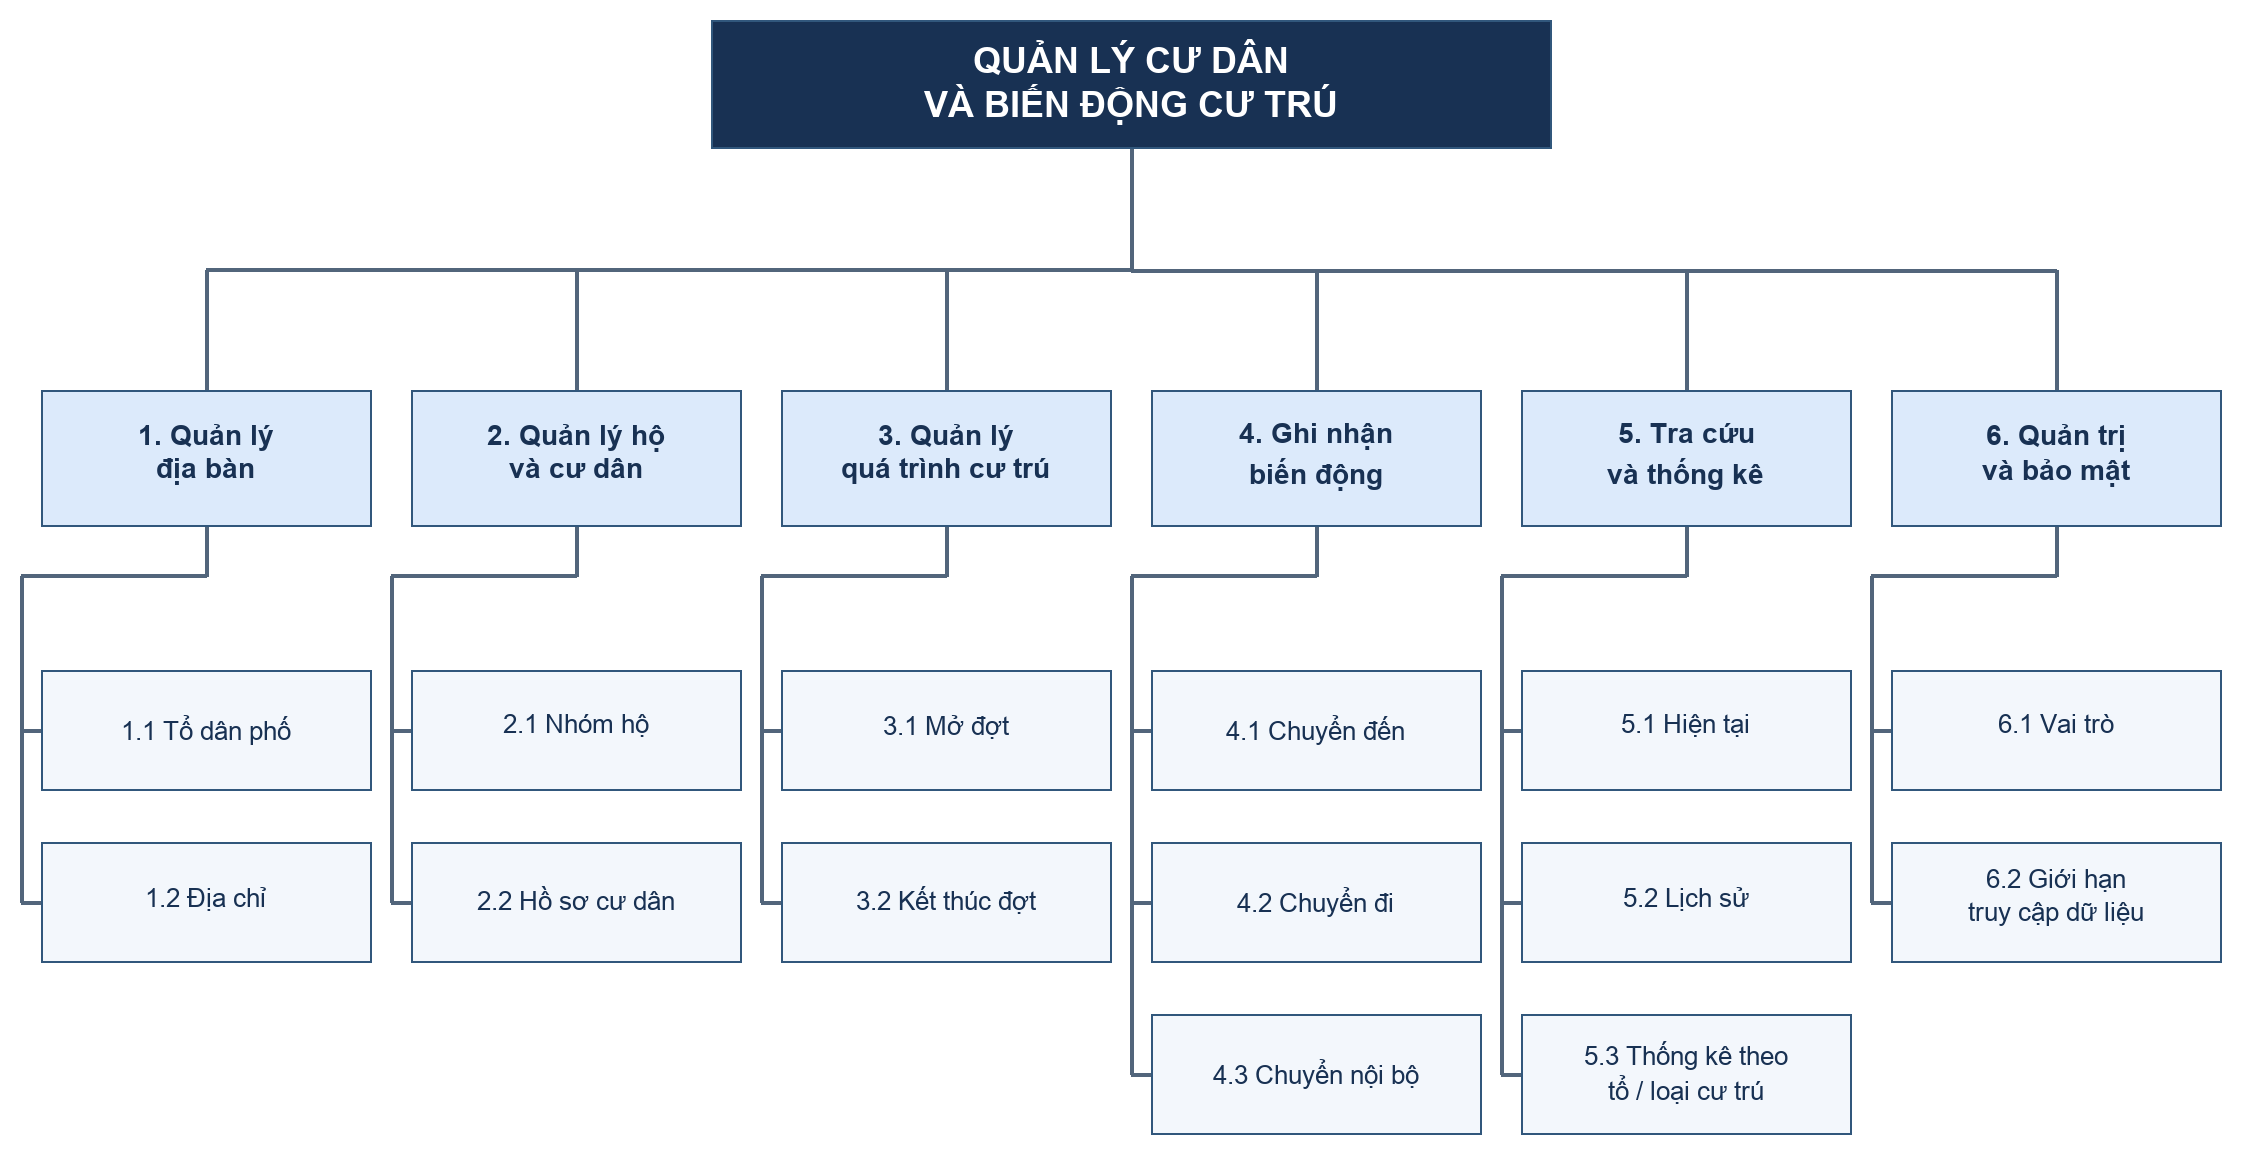
\includegraphics[width=\textwidth]{image/phan_ra_chuc_nang.png}
\caption{Sơ đồ phân rã chức năng của hệ thống quản lý cư dân và biến động cư trú}
\label{fig:bfd}
\end{figure}

Sơ đồ ở Hình \ref{fig:bfd} đọc từ trên xuống: ô trên cùng là toàn bộ hệ thống, hàng thứ hai là sáu nhóm chức năng, các ô dưới mỗi nhóm là 14 chức năng cấp 2 mà người dùng trực tiếp sử dụng.

\newpage

\section{MÔ HÌNH THỰC THỂ LIÊN KẾT}
\label{sec:chuong2}

Nhóm vẽ mô hình theo ký hiệu Chen trên công cụ ERDPlus: hình chữ nhật là thực thể, hình elip là thuộc tính (attribute), hình thoi là mối liên kết, thuộc tính gạch chân là thuộc tính khóa, còn thuộc tính có đánh dấu (O) là thuộc tính tùy chọn, có thể để trống. Chữ 1 và N trên đường nối cho biết bản số của mỗi phía trong liên kết.

\begin{figure}[H]
\centering
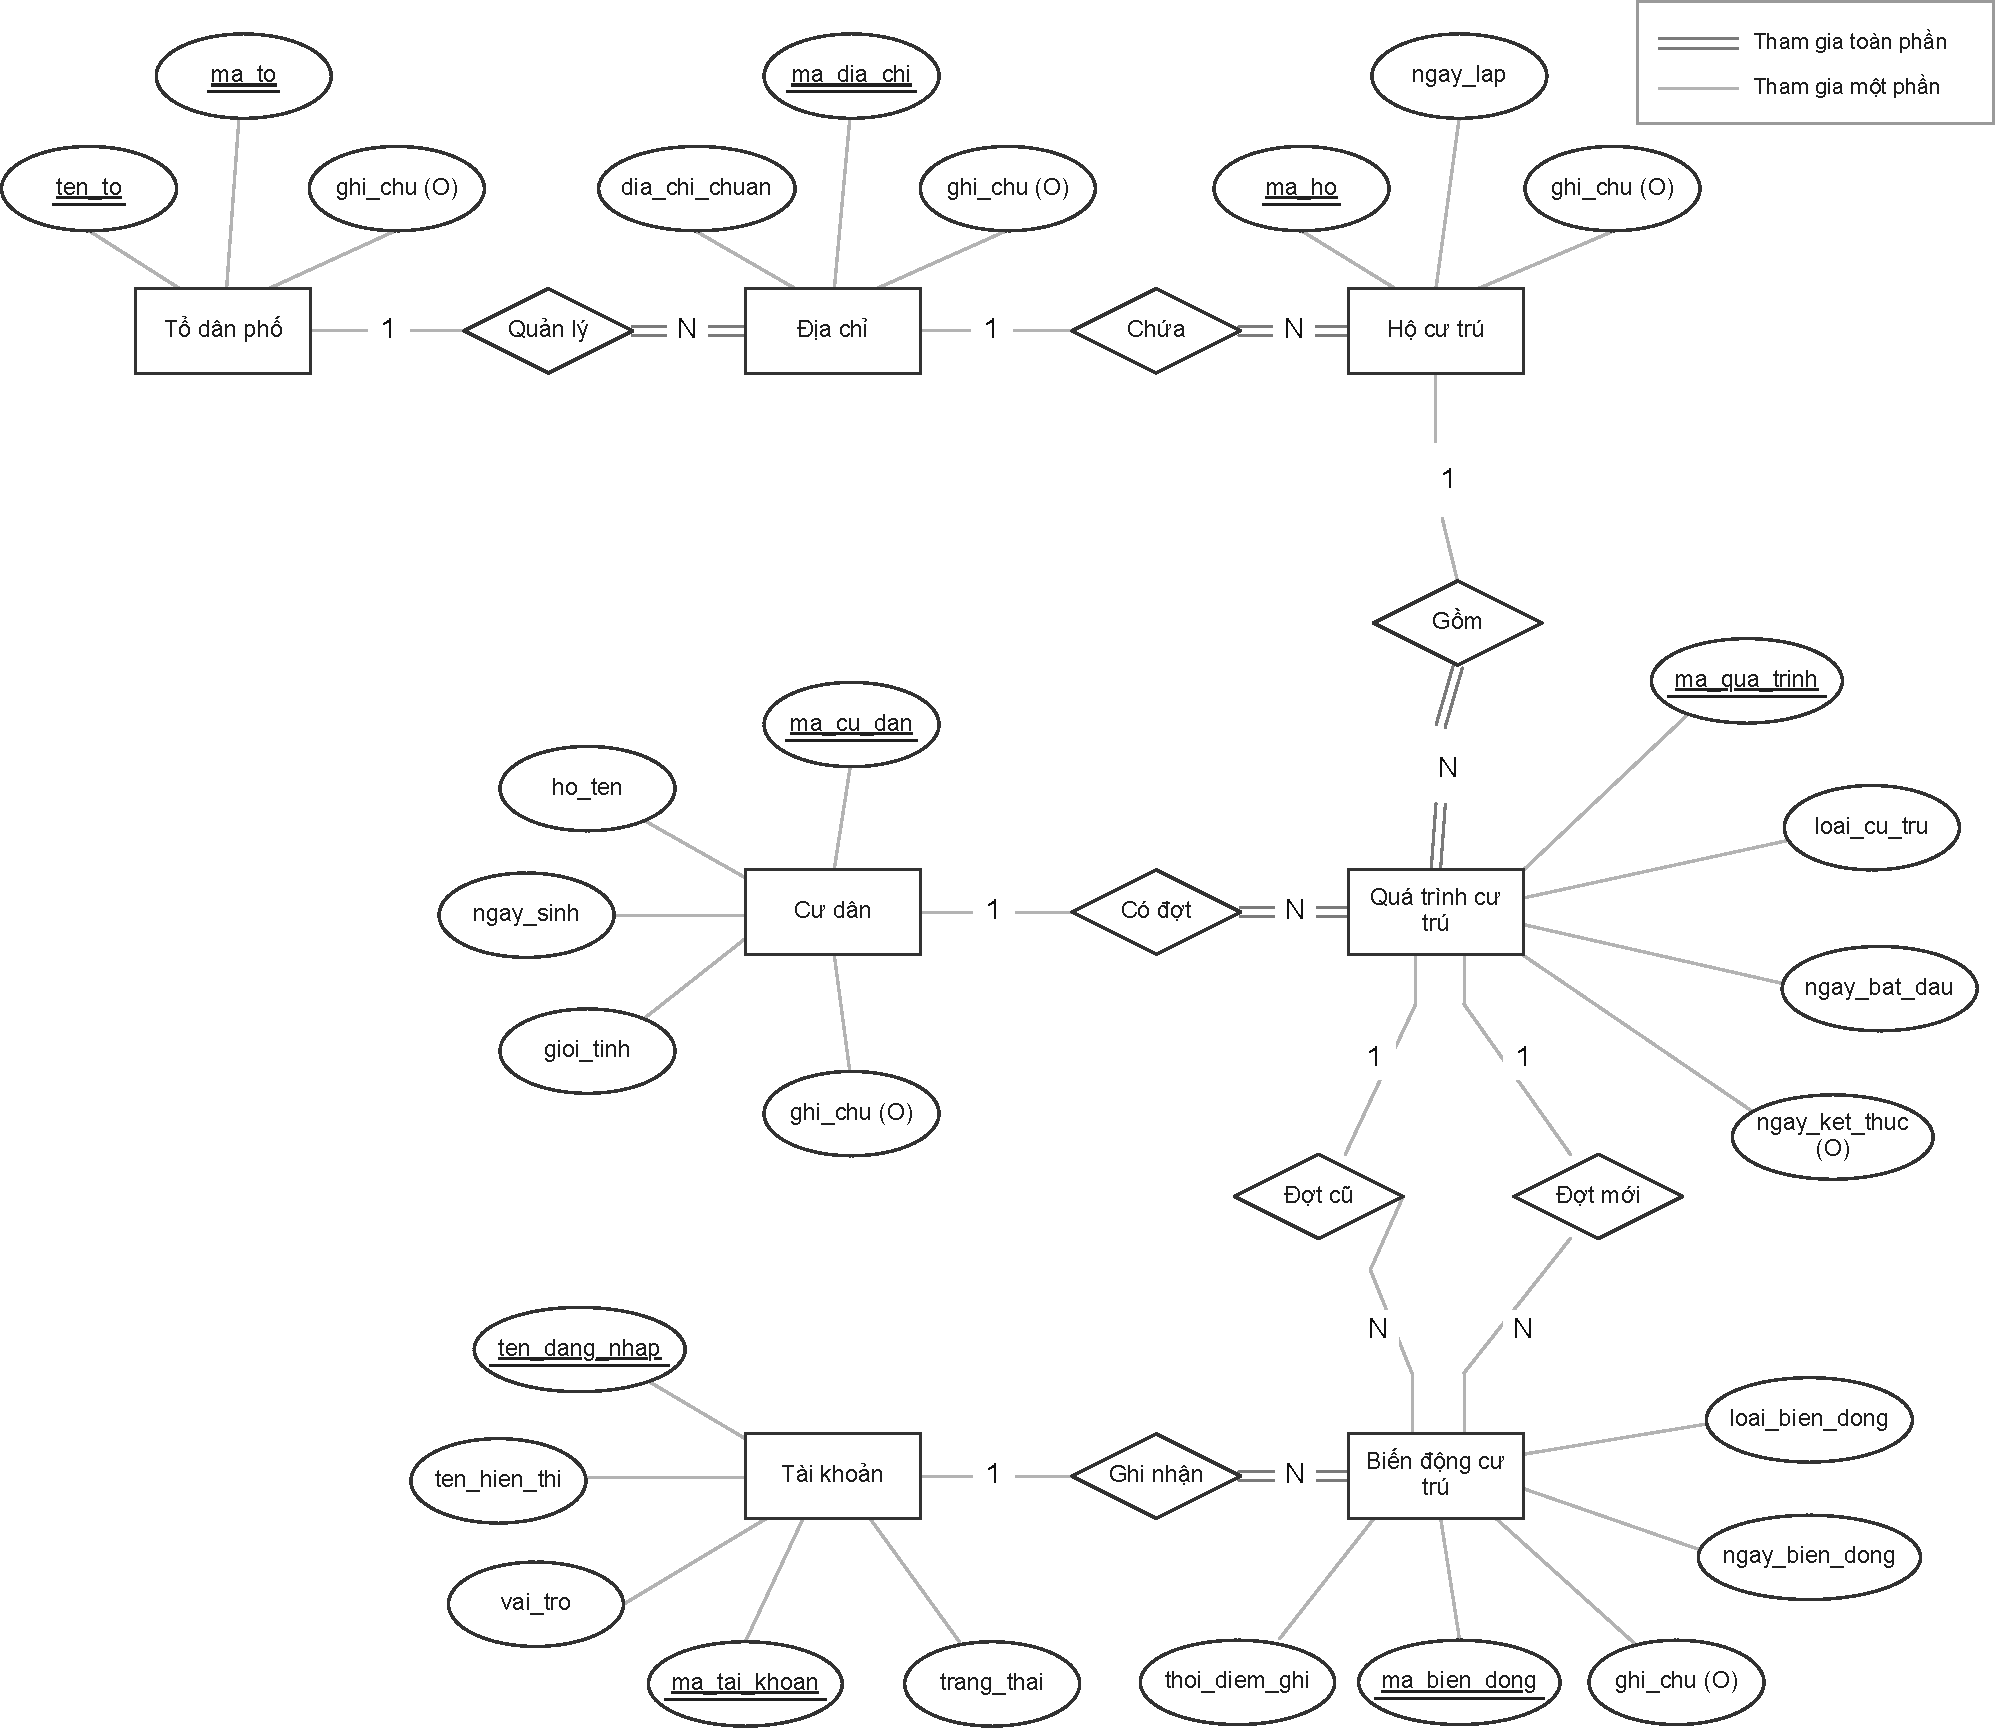
\includegraphics[width=\textwidth]{image/erd_trang_11_vector_crop.pdf}
\caption{Mô hình thực thể liên kết của hệ thống quản lý cư trú tổ dân phố}
\label{fig:erd}
\end{figure}

\subsection{Các thực thể và thuộc tính}
\label{subsec:thucthe}

\begin{table}[H]
\centering
\fontsize{12pt}{16pt}\selectfont
\renewcommand{\arraystretch}{1.15}
\begin{tabularx}{\textwidth}{|P{2.4cm}|Y|P{3.3cm}|P{3.6cm}|}
\hline
\textbf{Thực thể} & \textbf{Ý nghĩa} & \textbf{Thuộc tính khóa} & \textbf{Các thuộc tính còn lại} \\
\hline
Tổ dân phố & Một tổ dân phố thuộc phường & ma\_to; ten\_to cũng là duy nhất & ghi\_chu (O) \\
\hline
Địa chỉ & Một địa chỉ nhà nằm trong tổ, ghi theo dạng chuẩn; cặp (tổ, địa chỉ chuẩn) không trùng & ma\_dia\_chi & dia\_chi\_chuan, ghi\_chu (O) \\
\hline
Hộ cư trú & Một hộ cư trú gắn với một địa chỉ, có thể chưa phát sinh đợt cư trú & ma\_ho & ngay\_lap, ghi\_chu (O) \\
\hline
Cư dân & Một cá nhân có hồ sơ trong CSDL, có thể chưa phát sinh đợt cư trú & ma\_cu\_dan & ho\_ten, ngay\_sinh, gioi\_tinh, ghi\_chu (O) \\
\hline
Quá trình cư trú & Một đợt cư trú của một cư dân trong một hộ & ma\_qua\_trinh & loai\_cu\_tru, ngay\_bat\_dau, ngay\_ket\_thuc (O) \\
\hline
Biến động cư trú & Một lần thay đổi cư trú được cán bộ ghi nhận & ma\_bien\_dong & loai\_bien\_dong, ngay\_bien\_dong, thoi\_diem\_ghi, ghi\_chu (O) \\
\hline
Tài khoản & Tài khoản của cán bộ sử dụng hệ thống & ma\_tai\_khoan; ten\_dang\_nhap cũng là duy nhất & ten\_hien\_thi, vai\_tro, trang\_thai \\
\hline
\end{tabularx}
\caption{Các thực thể và thuộc tính}
\label{tab:thucthe}
\end{table}

Thực thể Quá trình cư trú là trung tâm của mô hình, vì nó cho biết một cư dân ở trong hộ nào, theo diện thường trú hay tạm trú và trong khoảng thời gian nào. Khi chuyển nội bộ, hệ thống đóng đợt cũ và mở đợt mới trong phường; khi chuyển ra ngoài phường, hệ thống chỉ đóng đợt cũ. Các đợt được lưu riêng để tra cứu lịch sử đã ghi nhận; việc bảo vệ chúng còn phụ thuộc quyền cập nhật và các trigger.

\subsection{Các mối liên kết}
\label{subsec:lienket}

\begin{table}[H]
\centering
\fontsize{12pt}{16pt}\selectfont
\renewcommand{\arraystretch}{1.15}
\begin{tabularx}{\textwidth}{|P{2.0cm}|P{2.5cm}|P{2.5cm}|Y|}
\hline
\textbf{Liên kết} & \textbf{Thực thể phía 1} & \textbf{Thực thể phía N} & \textbf{Giải thích} \\
\hline
Quản lý & Tổ dân phố & Địa chỉ & Một tổ quản lý nhiều địa chỉ, mỗi địa chỉ thuộc đúng một tổ \\
\hline
Chứa & Địa chỉ & Hộ cư trú & Một địa chỉ có thể có nhiều hộ, mỗi hộ ở đúng một địa chỉ \\
\hline
Gồm & Hộ cư trú & Quá trình cư trú & Một hộ gồm nhiều quá trình cư trú của các thành viên \\
\hline
Có đợt & Cư dân & Quá trình cư trú & Một cư dân có nhiều đợt cư trú theo thời gian \\
\hline
Ghi nhận & Tài khoản & Biến động cư trú & Biến động được ghi bằng đúng một tài khoản ở trạng thái hoạt động tại thời điểm ghi nhận (B14) \\
\hline
Đợt cũ & Quá trình cư trú & Biến động cư trú & Biến động làm kết thúc một quá trình (có thể không có, ví dụ chuyển đến) \\
\hline
Đợt mới & Quá trình cư trú & Biến động cư trú & Biến động mở ra một quá trình mới (có thể không có, ví dụ chuyển đi) \\
\hline
\end{tabularx}
\caption{Các mối liên kết trong mô hình}
\label{tab:lienket}
\end{table}

Giữa Quá trình cư trú và Biến động cư trú có hai liên kết song song là Đợt cũ và Đợt mới, vì một lần biến động có thể đóng một đợt cư trú và mở một đợt khác cùng lúc. Trường hợp điển hình là chuyển nội bộ: cư dân rời hộ A (đợt cũ kết thúc ngày $t-1$) và vào hộ B (đợt mới bắt đầu ngày $t$), cả hai đều gắn với cùng một bản ghi biến động.

\newpage
\section{THIẾT KẾ CƠ SỞ DỮ LIỆU}
\label{sec:chuong3}

\subsection{Các quy tắc ánh xạ đã áp dụng}
\label{subsec:anhxa}

Nhóm chuyển mô hình thực thể liên kết sang mô hình dữ liệu quan hệ theo hai quy tắc chính \cite{elmasri,silberschatz}. Thứ nhất, mỗi thực thể mạnh trở thành một bảng (quan hệ), các thuộc tính đơn trở thành các cột và thuộc tính khóa trở thành khóa chính (primary key); những thuộc tính cũng có giá trị duy nhất như ten\_to hay ten\_dang\_nhap được giữ làm khóa dự tuyển bằng ràng buộc UNIQUE. Thứ hai, với mỗi liên kết 1 -- N, nhóm đưa khóa chính của bảng phía 1 sang bảng phía N làm khóa ngoại (foreign key), nên cả 7 liên kết đều không cần tạo thêm bảng trung gian. Kết quả là 7 bảng, 35 cột, 7 khóa chính và 7 khóa ngoại.

Riêng hai liên kết Đợt cũ và Đợt mới cùng nối Quá trình cư trú với Biến động cư trú, nên bảng bien\_dong\_cu\_tru nhận hai khóa ngoại cùng trỏ về qua\_trinh\_cu\_tru và nhóm đặt tên khác nhau là ma\_qua\_trinh\_cu và ma\_qua\_trinh\_moi để phân biệt vai trò. Hai cột này cho phép NULL vì một biến động có thể chỉ có đợt cũ hoặc chỉ có đợt mới, trong khi các khóa ngoại còn lại đều là NOT NULL do phía 1 của liên kết là bắt buộc.

Mọi khóa chính đều dùng kiểu BIGINT GENERATED BY DEFAULT AS IDENTITY. Identity hỗ trợ cấp mã tự động; ràng buộc PRIMARY KEY bảo đảm tính duy nhất. Vì BY DEFAULT vẫn cho phép nhập mã tường minh, khi nạp dữ liệu có sẵn cần đồng bộ sequence để lần cấp mã tiếp theo không xung đột \cite{pgidentity}. Các giá trị liệt kê như loại cư trú hay loại biến động được lưu bằng mã không dấu (THUONG\_TRU, CHUYEN\_NOI\_BO\ldots) để so sánh ổn định, không phụ thuộc cách gõ dấu tiếng Việt.

\subsection{Lược đồ quan hệ}
\label{subsec:luocdo}

Trong lược đồ, gạch chân biểu thị khóa chính và chữ nghiêng biểu thị khóa ngoại.

{\sloppy
\begin{itemize}[leftmargin=*]
    \item to\_dan\_pho(\underline{ma\_to}, ten\_to, ghi\_chu)
    \item dia\_chi(\underline{ma\_dia\_chi}, \textit{ma\_to}, dia\_chi\_chuan, ghi\_chu)
    \item ho\_cu\_tru(\underline{ma\_ho}, \textit{ma\_dia\_chi}, ngay\_lap, ghi\_chu)
    \item cu\_dan(\underline{ma\_cu\_dan}, ho\_ten, ngay\_sinh, gioi\_tinh, ghi\_chu)
    \item qua\_trinh\_cu\_tru(\underline{ma\_qua\_trinh}, \textit{ma\_cu\_dan}, \textit{ma\_ho}, loai\_cu\_tru, ngay\_bat\_dau, ngay\_ket\_thuc)
    \item tai\_khoan(\underline{ma\_tai\_khoan}, ten\_dang\_nhap, ten\_hien\_thi, vai\_tro, trang\_thai)
    \item bien\_dong\_cu\_tru(\underline{ma\_bien\_dong}, loai\_bien\_dong, \textit{ma\_qua\_trinh\_cu}, \textit{ma\_qua\_trinh\_moi}, ngay\_bien\_dong, \textit{ma\_tai\_khoan}, thoi\_diem\_ghi, ghi\_chu)
\end{itemize}
\par}

\subsection{Cấu trúc các bảng}
\label{subsec:cautruc}

Nhóm cài đặt cơ sở dữ liệu trên PostgreSQL phiên bản 17. Các cột tên và địa chỉ dùng kiểu \texttt{VARCHAR}. Các cột ghi chú dùng kiểu \texttt{TEXT}. Mã hóa UTF-8 hỗ trợ lưu tiếng Việt. Các bảng \ref{tab:todanpho} đến \ref{tab:biendong} mô tả chi tiết từng bảng.

% Định dạng chung cho bảng cấu trúc
\newcommand{\bangcot}{\begin{tabularx}{\textwidth}{|P{3.3cm}|P{3.3cm}|P{3.5cm}|Y|}}
\newcommand{\dongtieude}{\hline \textbf{Cột} & \textbf{Kiểu dữ liệu} & \textbf{Ràng buộc} & \textbf{Mô tả} \\ \hline}

\begin{table}[H]
\centering
\fontsize{12pt}{16pt}\selectfont
\renewcommand{\arraystretch}{1.15}
\bangcot
\dongtieude
ma\_to & BIGINT & PK, tự tăng & Mã tổ dân phố \\ \hline
ten\_to & VARCHAR(60) & NOT NULL, UNIQUE, không rỗng & Tên tổ, không trùng nhau \\ \hline
ghi\_chu & TEXT & NULL & Ghi chú \\ \hline
\end{tabularx}
\caption{Cấu trúc bảng to\_dan\_pho -- lưu danh sách tổ dân phố}
\label{tab:todanpho}
\end{table}

\begin{table}[H]
\centering
\fontsize{12pt}{16pt}\selectfont
\renewcommand{\arraystretch}{1.15}
\bangcot
\dongtieude
ma\_dia\_chi & BIGINT & PK, tự tăng & Mã địa chỉ \\ \hline
ma\_to & BIGINT & NOT NULL, FK $\rightarrow$ to\_dan\_pho & Tổ quản lý địa chỉ \\ \hline
dia\_chi\_chuan & VARCHAR(200) & NOT NULL, không rỗng; UNIQUE cùng ma\_to & Địa chỉ ghi theo dạng chuẩn \\ \hline
ghi\_chu & TEXT & NULL & Ghi chú \\ \hline
\end{tabularx}
\caption{Cấu trúc bảng dia\_chi -- lưu các địa chỉ thuộc từng tổ}
\label{tab:diachi}
\end{table}

\begin{table}[H]
\centering
\fontsize{12pt}{16pt}\selectfont
\renewcommand{\arraystretch}{1.15}
\bangcot
\dongtieude
ma\_ho & BIGINT & PK, tự tăng & Mã hộ \\ \hline
ma\_dia\_chi & BIGINT & NOT NULL, FK $\rightarrow$ dia\_chi & Địa chỉ nơi hộ sinh sống \\ \hline
ngay\_lap & DATE & NOT NULL & Ngày lập hộ \\ \hline
ghi\_chu & TEXT & NULL & Ghi chú \\ \hline
\end{tabularx}
\caption{Cấu trúc bảng ho\_cu\_tru -- lưu các hộ cư trú}
\label{tab:hocutru}
\end{table}

\begin{table}[H]
\centering
\fontsize{12pt}{16pt}\selectfont
\renewcommand{\arraystretch}{1.15}
\bangcot
\dongtieude
ma\_cu\_dan & BIGINT & PK, tự tăng & Mã cư dân \\ \hline
ho\_ten & VARCHAR(120) & NOT NULL, không rỗng & Họ và tên \\ \hline
ngay\_sinh & DATE & NOT NULL & Ngày sinh \\ \hline
gioi\_tinh & VARCHAR(10) & NOT NULL, CHECK (Nam, Nu, Khac) & Giới tính \\ \hline
ghi\_chu & TEXT & NULL & Ghi chú \\ \hline
\end{tabularx}
\caption{Cấu trúc bảng cu\_dan -- lưu thông tin cá nhân của cư dân}
\label{tab:cudan}
\end{table}

\begin{table}[H]
\centering
\fontsize{12pt}{16pt}\selectfont
\renewcommand{\arraystretch}{1.15}
\bangcot
\dongtieude
ma\_qua\_trinh & BIGINT & PK, tự tăng & Mã quá trình cư trú \\ \hline
ma\_cu\_dan & BIGINT & NOT NULL, FK $\rightarrow$ cu\_dan & Cư dân của đợt cư trú \\ \hline
ma\_ho & BIGINT & NOT NULL, FK $\rightarrow$ ho\_cu\_tru & Hộ mà cư dân cư trú \\ \hline
loai\_cu\_tru & VARCHAR(20) & NOT NULL, CHECK (THUONG\_TRU, TAM\_TRU) & Loại cư trú \\ \hline
ngay\_bat\_dau & DATE & NOT NULL & Ngày bắt đầu đợt cư trú \\ \hline
ngay\_ket\_thuc & DATE & NULL, $\geq$ ngay\_bat\_dau & Ngày kết thúc; NULL nghĩa là chưa kết thúc \\ \hline
\end{tabularx}
\caption{Cấu trúc bảng qua\_trinh\_cu\_tru -- lưu từng đợt cư trú của cư dân trong hộ}
\label{tab:quatrinh}
\end{table}

\begin{table}[H]
\centering
\fontsize{12pt}{16pt}\selectfont
\renewcommand{\arraystretch}{1.15}
\bangcot
\dongtieude
ma\_tai\_khoan & BIGINT & PK, tự tăng & Mã tài khoản \\ \hline
ten\_dang\_nhap & VARCHAR(60) & NOT NULL, UNIQUE, không rỗng & Tên đăng nhập \\ \hline
ten\_hien\_thi & VARCHAR(120) & NOT NULL, không rỗng & Tên hiển thị của cán bộ \\ \hline
vai\_tro & VARCHAR(20) & NOT NULL, CHECK (QUAN\_TRI, CAN\_BO, THONG\_KE) & Vai trò nghiệp vụ của người ghi \\ \hline
trang\_thai & VARCHAR(20) & NOT NULL, mặc định HOAT\_DONG, CHECK (HOAT\_DONG, KHOA) & Trạng thái tài khoản \\ \hline
\end{tabularx}
\caption{Cấu trúc bảng tai\_khoan -- lưu tài khoản cán bộ sử dụng hệ thống}
\label{tab:taikhoan}
\end{table}

\begin{table}[H]
\centering
\fontsize{12pt}{16pt}\selectfont
\renewcommand{\arraystretch}{1.15}
\bangcot
\dongtieude
ma\_bien\_dong & BIGINT & PK, tự tăng & Mã biến động \\ \hline
loai\_bien\_dong & VARCHAR(20) & NOT NULL & CHUYEN\_DEN, CHUYEN\_DI hoặc CHUYEN\_NOI\_BO \\ \hline
ma\_qua\_trinh\_cu & BIGINT & NULL, FK $\rightarrow$ qua\_trinh\_cu\_tru & Đợt cư trú bị kết thúc \\ \hline
ma\_qua\_trinh\_moi & BIGINT & NULL, FK $\rightarrow$ qua\_trinh\_cu\_tru & Đợt cư trú được mở \\ \hline
ngay\_bien\_dong & DATE & NOT NULL & Ngày biến động xảy ra \\ \hline
ma\_tai\_khoan & BIGINT & NOT NULL, FK $\rightarrow$ tai\_khoan & Tài khoản ghi nhận \\ \hline
thoi\_diem\_ghi & TIMESTAMPTZ & NOT NULL, mặc định CURRENT\_TIMESTAMP & Thời điểm nhập vào hệ thống \\ \hline
ghi\_chu & TEXT & NULL & Ghi chú \\ \hline
\end{tabularx}
\caption{Cấu trúc bảng bien\_dong\_cu\_tru -- lưu lịch sử biến động cư trú}
\label{tab:biendong}
\end{table}

\subsection{Khóa, phụ thuộc hàm và chuẩn hóa}
\label{subsec:chuanhoa}

Nhóm phân tích chuẩn hóa dựa trên khóa ứng viên và phụ thuộc hàm (FD) của từng bảng \cite{elmasri,silberschatz}. Mỗi khóa chính xác định mọi thuộc tính còn lại trong bảng. Ngoài ra, \texttt{ten\_to} là khóa ứng viên của bảng tổ; cặp (\texttt{ma\_to}, \texttt{dia\_chi\_chuan}) là khóa ứng viên của bảng địa chỉ; \texttt{ten\_dang\_nhap} là khóa ứng viên của bảng tài khoản. Các khóa này đều được bảo đảm bởi NOT NULL và UNIQUE. B06 còn bảo đảm bộ (\texttt{ma\_cu\_dan}, \texttt{loai\_cu\_tru}, \texttt{ngay\_bat\_dau}) định danh một đợt: hai đợt cùng người, cùng loại và cùng ngày bắt đầu sẽ chồng lấn nên bị từ chối.

Ví dụ, \texttt{ma\_dia\_chi} xác định \texttt{ma\_to}, \texttt{dia\_chi\_chuan} và \texttt{ghi\_chu}; cặp tổ và địa chỉ chuẩn cũng xác định mã địa chỉ cùng ghi chú. \texttt{ma\_ho} xác định địa chỉ và ngày lập hộ; \texttt{ma\_cu\_dan} xác định thông tin hồ sơ; \texttt{ma\_qua\_trinh} xác định cư dân, hộ, loại và khoảng ngày của đợt. Tên tổ, địa chỉ dạng chữ và tên tài khoản được lưu ở bảng tương ứng, không sao chép vào bảng đợt hoặc sự kiện.

\begin{itemize}[leftmargin=*]
    \item \textbf{1NF:} mỗi ô chứa một giá trị, không lưu danh sách thành viên trong một cột; các lần cư trú được tách thành các dòng riêng. Với thuộc tính tùy chọn, CSDL dùng NULL theo ngữ nghĩa SQL; khi vận dụng đại số quan hệ cổ điển cần chuẩn bị đầu vào như mục \ref{subsec:qd}.
    \item \textbf{2NF:} xét cả khóa chính lẫn khóa ứng viên ghép. Với địa chỉ, mã và ghi chú của bản ghi phụ thuộc đầy đủ vào cặp tổ và địa chỉ chuẩn. Với đợt cư trú, không có FD được công bố từ một phần thực sự của khóa ghép nêu trên tới thuộc tính không khóa; chẳng hạn một cư dân hoặc một loại cư trú riêng lẻ không xác định hộ hay ngày kết thúc.
    \item \textbf{3NF:} theo tập FD đã công bố, sáu bảng tổ, địa chỉ, hộ, cư dân, quá trình cư trú và tài khoản không có FD không tầm thường với vế trái không là siêu khóa và vế phải là thuộc tính không khóa. Việc tách tên tổ, địa chỉ và thông tin tài khoản tránh cập nhật lặp lại các giá trị này ở nhiều bản ghi lịch sử.
\end{itemize}

\textbf{Ngày biến động và chuẩn hóa.} Xét các phụ thuộc hàm do khóa chính xác định, bảng biến động đáp ứng 3NF. B09 tạo thêm phụ thuộc có điều kiện trên các dòng có khóa ngoại đợt khác NULL. Nếu biến động có đợt mới, \texttt{ngay\_bien\_dong} bằng ngày bắt đầu đợt mới. Nếu có đợt cũ, ngày biến động bằng ngày kết thúc đợt cũ cộng một. Các khóa ngoại này có thể lặp, nên mã đợt xác định ngày biến động trong từng vai trò mà vẫn có thể tham chiếu từ nhiều bản ghi.

Nhóm lưu ngày biến động ngay trong bản ghi để tra cứu ngày nghiệp vụ. Trigger B09 kiểm tra sự nhất quán theo cả hai chiều. Phép kiểm E1 phát hiện một đợt được dùng lặp trong cùng vai trò.

\subsection{Các ràng buộc dữ liệu}
\label{subsec:rangbuoc}

Nhóm chia ràng buộc thành hai lớp. Lớp thứ nhất nằm ngay trong câu lệnh tạo bảng (tệp \texttt{sql/01\_schema.sql}), gồm khóa chính, khóa ngoại, UNIQUE và CHECK trên một dòng. Lớp thứ hai là các quy tắc liên quan tới nhiều dòng hoặc nhiều bảng mà CHECK không diễn đạt được, nhóm cài trong tệp \texttt{sql/02\_constraints.sql} bằng ràng buộc loại trừ (exclusion constraint), trigger và hàm PL/pgSQL.

\begin{enumerate}[leftmargin=*]
    \item \textbf{Miền giá trị (CHECK):} giới tính chỉ nhận Nam, Nu hoặc Khac; loại cư trú chỉ nhận THUONG\_TRU hoặc TAM\_TRU; vai trò và trạng thái tài khoản chỉ nhận các mã đã liệt kê; ngày kết thúc rỗng hoặc không sớm hơn ngày bắt đầu (B04). Tên tổ, địa chỉ, họ tên, tên đăng nhập và tên hiển thị không được rỗng hoặc chỉ toàn khoảng trắng (B15); năm ràng buộc CHECK này (\texttt{ck\_b15\_*}) được bổ sung trong \texttt{02\_constraints.sql}, nên sau khi chạy đủ hai tệp cơ sở dữ liệu có tổng cộng 11 ràng buộc CHECK.
    \item \textbf{Hình dạng biến động (B07):} ràng buộc \texttt{ck\_bd\_hinh\_dang} yêu cầu CHUYEN\_DEN chỉ có đợt mới, CHUYEN\_DI chỉ có đợt cũ, còn CHUYEN\_NOI\_BO có cả hai đợt và hai đợt này khác nhau.
    \item \textbf{Không chồng lấn đợt cư trú (B06):} nhóm dùng ràng buộc loại trừ \texttt{ex\_qt\_cu\_tru\_khong\_chong\_lan} với chỉ mục GiST (cần extension \texttt{btree\_gist}). Hai đợt cùng ma\_cu\_dan, cùng loai\_cu\_tru sẽ bị từ chối nếu khoảng ngày \texttt{daterange(ngay\_bat\_dau, ngay\_ket\_thuc, '[]')} của chúng giao nhau (toán tử \texttt{\&\&}); ngày kết thúc NULL được hiểu là không giới hạn.
    \item \textbf{Khớp sự kiện với đợt (B08, B09):} trigger \texttt{trg\_bien\_dong\_hop\_le} kiểm tra hai đợt của chuyển nội bộ cùng cư dân, khác hộ, đợt mới bắt đầu đúng ngày chuyển và đợt cũ kết thúc đúng ngày trước đó. Trigger \texttt{trg\_dot\_khong\_pha\_su\_kien} kiểm tra chiều ngược lại: sửa ngày của một đợt không được làm sai biến động đã ghi.
    \item \textbf{Giao dịch nguyên tử (B10):} hàm \texttt{fn\_chuyen\_noi\_bo} đóng đợt cũ, mở đợt mới và ghi biến động trong cùng một lần gọi; nếu một bước lỗi thì toàn bộ bị hủy.
    \item \textbf{Giữ địa chỉ lịch sử (B11):} trigger không cho đổi địa chỉ của một hộ, hay đổi tổ của một địa chỉ, khi đã có lịch sử cư trú tham chiếu tới.
    \item \textbf{Không xóa lịch sử (B12):} mọi khóa ngoại đều không CASCADE nên không xóa được hồ sơ đang được tham chiếu; ngoài ra role nghiệp vụ csdl17\_admin bị thu hồi quyền DELETE trên hai bảng lịch sử. Phạm vi quyền cập nhật được trình bày tại mục \ref{subsec:danhgia}.
    \item \textbf{Tài khoản hoạt động (B14):} trigger chỉ cho ghi biến động mới bằng tài khoản có trạng thái HOAT\_DONG; khóa tài khoản về sau không làm mất các biến động cũ.
    \item \textbf{Ngày hợp lý (B15):} trigger kiểm tra ngày sinh và ngày lập hộ không muộn hơn ngày bắt đầu các đợt cư trú, theo cả chiều ghi đợt và chiều sửa hồ sơ.
\end{enumerate}

Phép kiểm E1 trong \texttt{06\_validation.sql} phát hiện các biến động dùng lặp một đợt trong cùng vai trò. Điểm này cùng các giới hạn X01 và X06 được tổng hợp trong phần Kết luận.

Nhóm đã dựng lại cơ sở dữ liệu từ đầu trên PostgreSQL 17.12, chạy lần lượt \texttt{01\_schema.sql}, \texttt{02\_constraints.sql}, \texttt{03\_seed.sql} và \texttt{06\_validation.sql}; bước kiểm tra dữ liệu báo không có vi phạm B06, B08, B09, E1 và B15. Bộ dữ liệu mẫu nạp được 636 bản ghi: 8 tổ, 50 địa chỉ, 60 hộ, 200 cư dân, 250 đợt cư trú, 5 tài khoản và 63 biến động. Bảng \ref{tab:thurangbuoc} là kết quả thử một số câu lệnh cố tình vi phạm ràng buộc; mỗi lệnh chạy trong giao dịch được hoàn tác, và cột bên phải ghi đúng mã lỗi (SQLSTATE) cùng tên ràng buộc hoặc thông báo mà PostgreSQL trả về.

\begin{table}[H]
\centering
\fontsize{12pt}{16pt}\selectfont
\renewcommand{\arraystretch}{1.15}
\begin{tabularx}{\textwidth}{|Y|P{6.4cm}|}
\hline
\textbf{Thao tác thử} & \textbf{Kết quả của PostgreSQL} \\
\hline
Mở thêm đợt THUONG\_TRU cho cư dân 1 trùng thời gian với đợt đang có & Từ chối (23P01): vi phạm \texttt{ex\_qt\_cu\_tru\_khong\_chong\_lan} (B06) \\
\hline
Ghi CHUYEN\_DEN nhưng có cả đợt cũ: (a) đợt cũ là đợt 1 đang mở; (b) đợt cũ 16 kết thúc đúng ngày trước ngày chuyển, đợt mới 17 bắt đầu đúng ngày chuyển & Từ chối (23514). (a) Trigger B09 chặn trước: ``đợt cũ 1 phải kết thúc trước ngày chuyển 2026-10-15 đúng 1 ngày''. (b) Ngày khớp nên trigger cho qua, CHECK \texttt{ck\_bd\_hinh\_dang} (B07) chặn \\
\hline
Đổi địa chỉ của hộ 1 đã có lịch sử & Từ chối (23514): ``B11: không đổi địa chỉ của hộ 1 đã có lịch sử'' \\
\hline
Đợt có ngày kết thúc trước ngày bắt đầu & Từ chối (23514): vi phạm \texttt{ck\_qt\_ngay} \\
\hline
Xóa cư dân 1 đang có đợt cư trú & Từ chối (23503): vi phạm khóa ngoại \texttt{qua\_trinh\_cu\_tru\_ma\_cu\_dan\_fkey} \\
\hline
Thêm cư dân có họ tên chỉ gồm khoảng trắng & Từ chối (23514): vi phạm \texttt{ck\_b15\_ho\_ten} \\
\hline
\end{tabularx}
\caption{Kết quả thử các câu lệnh vi phạm ràng buộc}
\label{tab:thurangbuoc}
\end{table}

\subsection{Script tạo cơ sở dữ liệu}
\label{subsec:script}

Đoạn mã \ref{lst:schema} là phần tạo bảng trong \texttt{sql/01\_schema.sql}, kèm ràng buộc B06 lấy từ \texttt{sql/02\_constraints.sql}. Phụ lục~\hyperref[sec:phuluc]{A} trình bày mã nguồn các trigger và hàm tiêu biểu. Phần tạo bảng được chép nguyên văn từ tệp PostgreSQL của dự án, chỉ lược bỏ mệnh đề \texttt{IF NOT EXISTS} và năm câu lệnh tạo chỉ mục; ràng buộc B06 trong tệp gốc được bọc trong một khối \texttt{DO} kiểm tra tên ràng buộc để có thể chạy lại script nhiều lần.

\begin{lstlisting}[style=sqlvn, caption={Script tạo bảng và ràng buộc B06 trên PostgreSQL}, label={lst:schema}]
CREATE TABLE to_dan_pho (
    ma_to          BIGINT GENERATED BY DEFAULT AS IDENTITY PRIMARY KEY,
    ten_to         VARCHAR(60) NOT NULL UNIQUE,
    ghi_chu        TEXT
);

CREATE TABLE dia_chi (
    ma_dia_chi     BIGINT GENERATED BY DEFAULT AS IDENTITY PRIMARY KEY,
    ma_to          BIGINT NOT NULL REFERENCES to_dan_pho(ma_to),
    dia_chi_chuan  VARCHAR(200) NOT NULL,
    ghi_chu        TEXT,
    CONSTRAINT uq_dia_chi_to UNIQUE (ma_to, dia_chi_chuan)
);

CREATE TABLE ho_cu_tru (
    ma_ho          BIGINT GENERATED BY DEFAULT AS IDENTITY PRIMARY KEY,
    ma_dia_chi     BIGINT NOT NULL REFERENCES dia_chi(ma_dia_chi),
    ngay_lap       DATE NOT NULL,
    ghi_chu        TEXT
);

CREATE TABLE cu_dan (
    ma_cu_dan      BIGINT GENERATED BY DEFAULT AS IDENTITY PRIMARY KEY,
    ho_ten         VARCHAR(120) NOT NULL,
    ngay_sinh      DATE NOT NULL,
    gioi_tinh      VARCHAR(10) NOT NULL,
    ghi_chu        TEXT,
    CONSTRAINT ck_cu_dan_gioi_tinh CHECK (gioi_tinh IN ('Nam', 'Nu', 'Khac'))
);

CREATE TABLE qua_trinh_cu_tru (
    ma_qua_trinh   BIGINT GENERATED BY DEFAULT AS IDENTITY PRIMARY KEY,
    ma_cu_dan      BIGINT NOT NULL REFERENCES cu_dan(ma_cu_dan),
    ma_ho          BIGINT NOT NULL REFERENCES ho_cu_tru(ma_ho),
    loai_cu_tru    VARCHAR(20) NOT NULL,
    ngay_bat_dau   DATE NOT NULL,
    ngay_ket_thuc  DATE,
    CONSTRAINT ck_qt_loai CHECK (loai_cu_tru IN ('THUONG_TRU', 'TAM_TRU')),
    CONSTRAINT ck_qt_ngay CHECK (ngay_ket_thuc IS NULL OR ngay_ket_thuc >= ngay_bat_dau)
);

CREATE TABLE tai_khoan (
    ma_tai_khoan   BIGINT GENERATED BY DEFAULT AS IDENTITY PRIMARY KEY,
    ten_dang_nhap  VARCHAR(60) NOT NULL UNIQUE,
    ten_hien_thi   VARCHAR(120) NOT NULL,
    vai_tro        VARCHAR(20) NOT NULL,
    trang_thai     VARCHAR(20) NOT NULL DEFAULT 'HOAT_DONG',
    CONSTRAINT ck_tk_vai_tro CHECK (vai_tro IN ('QUAN_TRI', 'CAN_BO', 'THONG_KE')),
    CONSTRAINT ck_tk_trang_thai CHECK (trang_thai IN ('HOAT_DONG', 'KHOA'))
);

CREATE TABLE bien_dong_cu_tru (
    ma_bien_dong       BIGINT GENERATED BY DEFAULT AS IDENTITY PRIMARY KEY,
    loai_bien_dong     VARCHAR(20) NOT NULL,
    ma_qua_trinh_cu    BIGINT REFERENCES qua_trinh_cu_tru(ma_qua_trinh),
    ma_qua_trinh_moi   BIGINT REFERENCES qua_trinh_cu_tru(ma_qua_trinh),
    ngay_bien_dong     DATE NOT NULL,
    ma_tai_khoan       BIGINT NOT NULL REFERENCES tai_khoan(ma_tai_khoan),
    thoi_diem_ghi      TIMESTAMPTZ NOT NULL DEFAULT CURRENT_TIMESTAMP,
    ghi_chu            TEXT,
    CONSTRAINT ck_bd_hinh_dang CHECK (
        (loai_bien_dong = 'CHUYEN_DEN'
         AND ma_qua_trinh_cu IS NULL AND ma_qua_trinh_moi IS NOT NULL)
     OR (loai_bien_dong = 'CHUYEN_DI'
         AND ma_qua_trinh_cu IS NOT NULL AND ma_qua_trinh_moi IS NULL)
     OR (loai_bien_dong = 'CHUYEN_NOI_BO'
         AND ma_qua_trinh_cu IS NOT NULL AND ma_qua_trinh_moi IS NOT NULL
         AND ma_qua_trinh_cu <> ma_qua_trinh_moi)
    )
);

-- B06: cùng người, cùng loại cư trú thì khoảng ngày không được giao nhau
CREATE EXTENSION IF NOT EXISTS btree_gist;
ALTER TABLE qua_trinh_cu_tru
  ADD CONSTRAINT ex_qt_cu_tru_khong_chong_lan
  EXCLUDE USING gist (
    ma_cu_dan WITH =,
    loai_cu_tru WITH =,
    daterange(ngay_bat_dau, ngay_ket_thuc, '[]') WITH &&
  );
\end{lstlisting}

\subsection{Chỉ mục}
\label{subsec:chimuc}

PostgreSQL tự tạo chỉ mục B-tree cho khóa chính và ràng buộc UNIQUE. Nhóm bổ sung năm chỉ mục sau cho các cột thường dùng khi kết nối, lọc hoặc kiểm tra ràng buộc \cite{postgres}.

\begin{lstlisting}[style=sqlvn, caption={Năm chỉ mục bổ sung}, label={lst:chimuc}]
CREATE INDEX IF NOT EXISTS idx_dia_chi_to ON dia_chi(ma_to);
CREATE INDEX IF NOT EXISTS idx_ho_dia_chi ON ho_cu_tru(ma_dia_chi);
CREATE INDEX IF NOT EXISTS idx_qt_cu_dan_ngay ON qua_trinh_cu_tru(ma_cu_dan, ngay_bat_dau);
CREATE INDEX IF NOT EXISTS idx_qt_ho_ngay ON qua_trinh_cu_tru(ma_ho, ngay_bat_dau);
CREATE INDEX IF NOT EXISTS idx_bd_loai_ngay ON bien_dong_cu_tru(loai_bien_dong, ngay_bien_dong);
\end{lstlisting}

\begin{itemize}[leftmargin=*]
    \item \texttt{idx\_dia\_chi\_to} và \texttt{idx\_ho\_dia\_chi} hỗ trợ đường nối từ tổ đến địa chỉ và hộ, chẳng hạn khi thống kê theo tổ (QSQL03) hoặc tìm địa chỉ chưa có hộ (QSQL04).
    \item \texttt{idx\_qt\_cu\_dan\_ngay} hỗ trợ tra cứu đợt theo cư dân và khoảng ngày, chẳng hạn khi kiểm tra đợt còn hiệu lực ở QSQL07 hoặc khi trigger B15 kiểm tra ngày sinh.
    \item \texttt{idx\_qt\_ho\_ngay} hỗ trợ tìm các đợt của một hộ, chẳng hạn khi đếm người ở QSQL02 hoặc khi kiểm tra lịch sử của hộ theo B11.
    \item \texttt{idx\_bd\_loai\_ngay} phục vụ truy vấn lọc theo loại biến động và, khi cần, theo khoảng ngày. QSQL09 lọc chuyển nội bộ và sắp theo mã biến động. QSQL08 tổng hợp toàn bộ các loại theo tháng, nên chỉ mục này không bảo đảm truy vấn tránh quét bảng.
\end{itemize}

Với chỉ mục B-tree nhiều cột, đặt cột so sánh bằng ở đầu hỗ trợ tìm nhanh phần cần đọc, sau đó có thể giới hạn trên cột ngày. Lọc theo khoảng ngày tạo điều kiện dùng chỉ mục trên cột ngày. PostgreSQL cũng hỗ trợ chỉ mục trên biểu thức \cite{pgexpressionindex}. Trên bộ 636 bản ghi, lựa chọn kế hoạch phụ thuộc số dòng cần đọc và chi phí ước tính. Nhóm chưa đo mức cải thiện thời gian chạy.

\subsection{Câu lệnh DML minh họa}
\label{subsec:dml}

Ba ví dụ minh họa cách các ràng buộc ở mục \ref{subsec:rangbuoc} kiểm tra thao tác thêm và sửa dữ liệu. Nhóm chạy trên PostgreSQL 17.12 với cơ sở dữ liệu dựng mới từ schema, ràng buộc và bộ 636 bản ghi. Hai ví dụ đầu lấy ngày hệ thống làm ngày chuyển. Mỗi giao dịch được hoàn tác để giữ nguyên các bản ghi mẫu. Script và kết quả được lưu lần lượt tại \texttt{tests/report\_dml\_minh\_hoa.sql} và \texttt{tests/report\_dml\_minh\_hoa\_log.txt}.

\textbf{Ví dụ 1: chuyển nội bộ bằng hàm.} Cư dân 40 (Phạm Thu Hạnh) đang thường trú tại hộ 21 theo đợt 44. Cán bộ dùng tài khoản 2 ghi nhận người này chuyển thường trú sang hộ 2 từ hôm nay.

\begin{lstlisting}[style=sqlvn]
BEGIN;
SELECT * FROM fn_chuyen_noi_bo(44, 2, 'THUONG_TRU', CURRENT_DATE, 2);
ROLLBACK;
\end{lstlisting}

Hàm khóa đợt 44 bằng \texttt{FOR UPDATE}, đặt ngày kết thúc của đợt này là hôm qua, thêm đợt thường trú mới tại hộ 2 bắt đầu từ hôm nay, rồi ghi một biến động CHUYEN\_NOI\_BO trỏ tới cả hai đợt. Kết quả trả về là mã đợt mới và mã biến động vừa được cấp; trên cơ sở dữ liệu dựng mới, đó là đợt 251 và biến động 64. Khi biến động được ghi, trigger \texttt{trg\_bien\_dong\_hop\_le} vẫn kiểm tra lại B08, B09 và B14; nếu một bước lỗi thì cả ba thay đổi bị hủy (B10). Người dùng chỉ cần một lệnh, không phải tự viết ba câu UPDATE và INSERT theo đúng thứ tự.

\textbf{Ví dụ 2: ghi chuyển đi.} Cư dân 44 (Đặng Ngọc Chi) đang thường trú tại hộ 16 theo đợt 50 và chuyển ra khỏi phường từ hôm nay. Nhóm không viết hàm riêng cho trường hợp này, nên hai lệnh được đặt trong cùng một giao dịch.

\begin{lstlisting}[style=sqlvn]
BEGIN;
UPDATE qua_trinh_cu_tru
SET ngay_ket_thuc = CURRENT_DATE - 1
WHERE ma_qua_trinh = 50;

INSERT INTO bien_dong_cu_tru (loai_bien_dong, ma_qua_trinh_cu, ma_qua_trinh_moi,
                              ngay_bien_dong, ma_tai_khoan)
VALUES ('CHUYEN_DI', 50, NULL, CURRENT_DATE, 2);
ROLLBACK;
\end{lstlisting}

Thứ tự hai lệnh là bắt buộc. Nếu INSERT chạy trước khi đợt 50 được đóng, trigger B09 từ chối với lỗi 23514 ``B09: đợt cũ 50 phải kết thúc trước ngày chuyển \ldots{} đúng 1 ngày'', trong đó ngày chuyển là ngày chạy lệnh. Biến động CHUYEN\_DI chỉ có đợt cũ, đúng hình dạng mà CHECK \texttt{ck\_bd\_hinh\_dang} yêu cầu (B07).

\textbf{Ví dụ 3: UPDATE bị trigger chặn.} Đợt 17 là đợt mới của biến động 2, lần chuyển nội bộ ngày 15/10/2026 của cư dân 15. Câu lệnh sau thử dời ngày bắt đầu của đợt này sang 20/10/2026.

\begin{lstlisting}[style=sqlvn]
UPDATE qua_trinh_cu_tru
SET ngay_bat_dau = DATE '2026-10-20'
WHERE ma_qua_trinh = 17;
\end{lstlisting}

Trigger \texttt{trg\_dot\_khong\_pha\_su\_kien} kiểm tra lại các biến động đang trỏ tới đợt 17 và báo lỗi 23514: ``B09: đợt mới 17 phải bắt đầu đúng ngày chuyển 2026-10-15''. Dòng dữ liệu giữ nguyên, nên biến động 2 vẫn khớp với hai đợt mà nó trỏ tới.

\newpage
\section{TRUY VẤN BẰNG ĐẠI SỐ QUAN HỆ}
\label{sec:chuong4}

Để biểu thức gọn hơn, nhóm viết tắt tên các quan hệ như sau: TDP = to\_dan\_pho, DC = dia\_chi, HO = ho\_cu\_tru, CD = cu\_dan, QT = qua\_trinh\_cu\_tru, TK = tai\_khoan và BD = bien\_dong\_cu\_tru. Nhiều bảng cùng có cột ghi\_chu, nên nếu dùng phép kết nối tự nhiên (natural join) thì cột này cũng bị đem ra so sánh và cho kết quả sai. Vì vậy, ở các câu có kết nối, nhóm hoặc chiếu bớt cột trước khi kết nối, hoặc dùng phép kết nối theo điều kiện ($\theta$-join) ghi rõ cột cần so khớp.

\phantomsection
\label{subsec:qd}
Các câu hỏi về người đang cư trú xét hiệu lực theo quy tắc B05 tại ngày hiện tại của phiên PostgreSQL. Đại số quan hệ cổ điển không có NULL, nên nhóm chuẩn bị đầu vào bằng SQL trước khi áp dụng các phép toán. Quan hệ $Q_{\mathrm{ht}}$ gồm các đợt còn hiệu lực và chỉ giữ các cột bắt buộc:
\begin{equation*}
\begin{aligned}
Q_{\mathrm{ht}}(&\text{ma\_qua\_trinh},\ \text{ma\_cu\_dan},\ \text{ma\_ho},\\
    &\text{loai\_cu\_tru},\ \text{ngay\_bat\_dau})
\end{aligned}
\end{equation*}
Năm cột trên đều NOT NULL. Quan hệ $Q_{\mathrm{bd}}$ có cùng lược đồ nhưng gồm tất cả đợt đã bắt đầu. Bước chuẩn bị $Q_{\mathrm{bd}}$ lọc \texttt{ngay\_bat\_dau <= CURRENT\_DATE}; $Q_{\mathrm{ht}}$ còn yêu cầu ngày kết thúc để trống hoặc không trước \texttt{CURRENT\_DATE}. Cả hai dùng SELECT DISTINCT năm cột trên, không đưa cột ngày kết thúc vào đầu vào đại số. Cách xử lý này loại đợt chưa bắt đầu và giữ NULL ở ngoài các phép toán cổ điển.

\textbf{Câu 1.} Cho biết họ tên và ngày sinh của các cư dân nữ, phục vụ việc lập danh sách hoạt động của chi hội phụ nữ.
\begin{equation*}
\pi_{\text{ho\_ten},\ \text{ngay\_sinh}}\left(\sigma_{\text{gioi\_tinh} = \text{'Nu'}}(CD)\right)
\end{equation*}
Phép chọn $\sigma$ lọc ra các bộ có giới tính là Nu, sau đó phép chiếu $\pi$ chỉ giữ lại hai cột cần in. Nhóm đặt phép chọn ở trong và phép chiếu ở ngoài, vì nếu chiếu trước thì cột gioi\_tinh đã bị bỏ đi và không còn để lọc nữa.

\textbf{Câu 2.} Liệt kê mã và địa chỉ chuẩn của tất cả địa chỉ thuộc ``Tổ 01''.
\begin{equation*}
\begin{aligned}
R &\leftarrow \sigma_{\text{ten\_to} = \text{'Tổ 01'}}(TDP)\\
KQ &\leftarrow \pi_{\text{ma\_dia\_chi},\ \text{dia\_chi\_chuan}}\left(R \bowtie_{R.\text{ma\_to} = DC.\text{ma\_to}} DC\right)
\end{aligned}
\end{equation*}
Nhóm chọn tổ trước rồi mới kết nối để giảm số bộ ở đầu vào của phép kết nối theo biến đổi đại số. Đây là cách tổ chức biểu thức, không phải kết luận đo hiệu năng thực thi.

\textbf{Câu 3.} Cho biết mã và họ tên các cư dân đang thường trú tại tổ có mã 1. Biểu thức khá dài nên nhóm viết thành từng bước với các quan hệ trung gian.
\begin{equation*}
\begin{aligned}
R_1 &\leftarrow \sigma_{\text{loai\_cu\_tru} = \text{'THUONG\_TRU'}}(Q_{\mathrm{ht}})\\
R_2 &\leftarrow \pi_{\text{ma\_ho}}\left(HO \bowtie_{HO.\text{ma\_dia\_chi} = DC.\text{ma\_dia\_chi}} \sigma_{\text{ma\_to} = 1}(DC)\right)\\
R_3 &\leftarrow R_1 \bowtie_{R_1.\text{ma\_ho} = R_2.\text{ma\_ho}} R_2\\
KQ &\leftarrow \pi_{CD.\text{ma\_cu\_dan},\ \text{ho\_ten}}\left(R_3 \bowtie_{R_3.\text{ma\_cu\_dan} = CD.\text{ma\_cu\_dan}} CD\right)
\end{aligned}
\end{equation*}
$R_1$ là các đợt thường trú còn hiệu lực hiện tại, $R_2$ là các hộ nằm trong tổ 1; $R_3$ ghép hai kết quả này lại, và kết nối $R_3$ với CD là lấy được họ tên.

\textbf{Câu 4.} Tìm các cư dân đã từng cư trú trong phường nhưng hiện tại không còn đợt nào hiệu lực, để cán bộ rà soát lại hồ sơ.
\begin{equation*}
\begin{aligned}
R &\leftarrow \pi_{\text{ma\_cu\_dan}}\left(Q_{\mathrm{bd}}\right) - \pi_{\text{ma\_cu\_dan}}(Q_{\mathrm{ht}})\\
KQ &\leftarrow \pi_{\text{ma\_cu\_dan},\ \text{ho\_ten}}(R \bowtie CD)
\end{aligned}
\end{equation*}
Phép hiệu lấy những người có đợt đã bắt đầu trong $Q_{\mathrm{bd}}$, trừ đi những người còn đợt hiệu lực trong $Q_{\mathrm{ht}}$. Cả hai vế đều chiếu về mã cư dân, nên tương thích với phép hiệu. Ở bước sau, $R$ chỉ có cột ma\_cu\_dan nên dùng kết nối tự nhiên với CD là an toàn.

\textbf{Câu 5.} Cho biết mã các cư dân đã từng tạm trú và cũng đã từng thường trú trong phường.
\begin{equation*}
\begin{aligned}
A &\leftarrow \pi_{\text{ma\_cu\_dan}}\left(\sigma_{\text{loai\_cu\_tru} = \text{'TAM\_TRU'}}(QT)\right)\\
B &\leftarrow \pi_{\text{ma\_cu\_dan}}\left(\sigma_{\text{loai\_cu\_tru} = \text{'THUONG\_TRU'}}(QT)\right)\\
KQ &\leftarrow A \cap B
\end{aligned}
\end{equation*}
Không thể viết câu này bằng một phép chọn với điều kiện AND, vì mỗi bộ của QT chỉ có một loại cư trú; hai điều kiện phải đúng ở hai bộ khác nhau nên cần dùng phép giao.

\textbf{Câu 6.} Liệt kê mã tất cả các biến động có liên quan đến cư dân mã 92, dù cư dân này nằm ở đợt cũ hay đợt mới của biến động.
\begin{equation*}
\begin{aligned}
Q &\leftarrow \pi_{\text{ma\_qua\_trinh}}\left(\sigma_{\text{ma\_cu\_dan} = 92}(QT)\right)\\
KQ &\leftarrow \pi_{\text{ma\_bien\_dong}}\left(BD \bowtie_{\text{ma\_qua\_trinh\_cu} = \text{ma\_qua\_trinh}} Q\right)\\
&\phantom{\leftarrow}\ \cup\ \pi_{\text{ma\_bien\_dong}}\left(BD \bowtie_{\text{ma\_qua\_trinh\_moi} = \text{ma\_qua\_trinh}} Q\right)
\end{aligned}
\end{equation*}
Vế trái của phép hợp lấy các biến động mà cư dân 92 rời đi, vế phải lấy các biến động mà cư dân 92 đến; một lần chuyển nội bộ sẽ xuất hiện ở cả hai vế nhưng phép hợp tự loại bỏ bộ trùng.

\textbf{Câu 7.} Với mỗi biến động chuyển nội bộ, cho biết họ tên cư dân, mã hộ cũ và mã hộ mới.
\begin{equation*}
\begin{aligned}
QC &\leftarrow \rho_{QC(\text{mq\_cu},\ \text{ho\_cu})}\left(\pi_{\text{ma\_qua\_trinh},\ \text{ma\_ho}}(QT)\right)\\
P &\leftarrow \pi_{\text{ma\_qua\_trinh},\ \text{ma\_ho},\ \text{ma\_cu\_dan}}(QT)\\
QM &\leftarrow \rho_{QM(\text{mq\_moi},\ \text{ho\_moi},\ \text{ma\_cu\_dan})}(P)\\
R_0 &\leftarrow \sigma_{\text{loai\_bien\_dong} = \text{'CHUYEN\_NOI\_BO'}}(BD)\\
R_1 &\leftarrow R_0 \bowtie_{\text{ma\_qua\_trinh\_cu} = \text{mq\_cu}} QC\\
R &\leftarrow R_1 \bowtie_{\text{ma\_qua\_trinh\_moi} = \text{mq\_moi}} QM\\
KQ &\leftarrow \pi_{\text{ma\_bien\_dong},\ \text{ho\_ten},\ \text{ho\_cu},\ \text{ho\_moi}}\left(R \bowtie \pi_{\text{ma\_cu\_dan},\ \text{ho\_ten}}(CD)\right)
\end{aligned}
\end{equation*}
Vì một biến động tham chiếu tới QT hai lần với hai vai trò khác nhau, nhóm dùng phép đổi tên $\rho$ để tạo ra hai bản sao QC (đợt cũ) và QM (đợt mới) có tên cột khác nhau, nhờ đó kết nối được cả hai lần mà không bị trùng tên thuộc tính.

\textbf{Câu 8.} Cho biết tên hiển thị của những cán bộ đã ghi nhận biến động chuyển đi xảy ra trong tháng 10/2026.
\begin{equation*}
\begin{aligned}
R &\leftarrow \sigma_{\substack{\text{loai\_bien\_dong} = \text{'CHUYEN\_DI'}\\ \wedge\ \text{ngay\_bien\_dong} \ge \text{'2026-10-01'}\\ \wedge\ \text{ngay\_bien\_dong} \le \text{'2026-10-31'}}}(BD)\\
KQ &\leftarrow \pi_{\text{ten\_hien\_thi}}\left(R \bowtie_{R.\text{ma\_tai\_khoan} = TK.\text{ma\_tai\_khoan}} TK\right)
\end{aligned}
\end{equation*}
Phép chọn trên BD gộp ba điều kiện bằng phép hội $\wedge$ để lấy đúng loại biến động trong khoảng thời gian cần xét, rồi mới kết nối với TK để lấy tên cán bộ. Vì phép chiếu tự loại các bộ trùng nhau, một cán bộ ghi nhiều lần chuyển đi trong tháng cũng chỉ xuất hiện một lần trong kết quả.

\textbf{Câu 9.} Tìm những tài khoản đã ghi nhận đủ các loại biến động xuất hiện trong dữ liệu.
\begin{equation*}
\pi_{\text{ma\_tai\_khoan},\ \text{loai\_bien\_dong}}(BD) \div \pi_{\text{loai\_bien\_dong}}(BD)
\end{equation*}
Quan hệ bị chia $\pi_{\text{ma\_tai\_khoan},\ \text{loai\_bien\_dong}}(BD)$ gồm các cặp (tài khoản, loại biến động) đã từng được ghi; quan hệ chia $\pi_{\text{loai\_bien\_dong}}(BD)$ là tập các loại biến động có trong hệ thống. Kết quả có lược đồ là phần còn lại $\{\text{ma\_tai\_khoan}\}$, gồm những tài khoản mà khi ghép với \emph{mọi} bộ của quan hệ chia đều có mặt trong quan hệ bị chia. Đây là dạng câu hỏi có chữ ``tất cả'' mà các phép chọn, chiếu, kết nối thông thường không diễn đạt trực tiếp được. Quan hệ chia ở đây lấy từ dữ liệu đã ghi; nếu muốn hiểu ``tất cả loại'' theo miền giá trị của CHECK thì thay bằng quan hệ hằng gồm ba bộ CHUYEN\_DEN, CHUYEN\_DI, CHUYEN\_NOI\_BO. Trên bộ dữ liệu mẫu cả ba loại đều đã xuất hiện nên hai cách hiểu cho cùng kết quả. Nhóm kiểm chứng bằng hai câu SQL độc lập, một câu dùng hai lớp NOT EXISTS và một câu đếm số loại phân biệt của mỗi tài khoản: cả hai đều trả về bốn tài khoản 1, 2, 3, 4; tài khoản 5 chưa ghi biến động nào nên không có bộ nào trong quan hệ bị chia và không thể xuất hiện trong kết quả.

\textbf{Câu 10.} Đếm số nhân khẩu đang cư trú hiện tại của từng hộ.
\begin{equation*}
{}_{\text{ma\_ho}}\,\gamma_{\,\text{COUNT(ma\_cu\_dan)} \rightarrow \text{so\_nhan\_khau}}\left(\pi_{\text{ma\_ho},\ \text{ma\_cu\_dan}}(Q_{\mathrm{ht}})\right)
\end{equation*}
Phép gom nhóm $\gamma$ (một số giáo trình ký hiệu là $\Im$) không thuộc các phép toán của đại số quan hệ cổ điển mà thuộc \textbf{đại số quan hệ mở rộng}, vốn bổ sung phép gom nhóm và hàm tổng hợp như COUNT \cite{elmasri,silberschatz}. Phép này chia các cặp (hộ, cư dân) theo ma\_ho rồi đếm số cư dân trong mỗi nhóm. Nhóm chiếu về cặp (ma\_ho, ma\_cu\_dan) trước khi gom nhóm để một người có cả đợt thường trú và đợt tạm trú trong cùng hộ chỉ được đếm một lần, đúng với quy tắc B17 là số người phải tính theo mã cư dân phân biệt. Trên bộ dữ liệu mẫu hiện tại chưa có hộ nào rơi vào trường hợp này, nhưng phép chiếu vẫn cần để biểu thức đúng với mọi dữ liệu hợp lệ. Kết quả có 56 hộ đang có người hiện tại, trong đó 40 hộ có từ 3 nhân khẩu trở lên, khớp với câu 3 ở Chương \ref{sec:chuong5}.

\subsection*{Đối chiếu biểu thức đại số quan hệ với SQL}

Mỗi biểu thức được dịch sang SQL theo ngữ nghĩa tập hợp: phép chiếu dùng SELECT DISTINCT; hợp, giao, hiệu lần lượt dùng UNION, INTERSECT, EXCEPT; phép chia dùng hai lớp NOT EXISTS; phép gom nhóm dùng GROUP BY. Các câu tương ứng ở Chương \ref{sec:chuong5} được so sánh tập kết quả theo cả hai chiều. Bảng \ref{tab:doichieura} trình bày số liệu minh họa trên bộ dữ liệu mẫu tại thời điểm thực nghiệm. Các kết quả về cư trú hiện tại có thể thay đổi theo ngày hệ thống; việc kiểm chứng đối chiếu truy vấn dùng cùng ngày hệ thống, không gắn kết quả với một ngày cố định.

\begin{table}[H]
\centering
\fontsize{11pt}{14pt}\selectfont
\renewcommand{\arraystretch}{1.15}
\begin{tabularx}{\textwidth}{|P{1.3cm}|P{2.4cm}|Y|}
\hline
\textbf{Câu} & \textbf{Số bộ kết quả} & \textbf{Đối chiếu} \\
\hline
1 & 98 & Bằng số cư dân nữ (không có hai người nữ trùng cả họ tên và ngày sinh) \\
\hline
2 & 8 & Bằng số địa chỉ thuộc Tổ 01 \\
\hline
3 & 23 & Trùng khớp từng bộ với câu 1 Chương \ref{sec:chuong5} \\
\hline
4 & 17 & Trùng khớp từng bộ với câu 4 Chương \ref{sec:chuong5} \\
\hline
5 & 31 & Bằng số dòng của câu 9 Chương \ref{sec:chuong5}, vốn dùng cùng phép INTERSECT \\
\hline
6 & 1 (biến động 32) & Lần chuyển nội bộ ngày 02/7/2026 từ hộ 56 sang hộ 20; trùng với cách viết một phép chọn dùng điều kiện ``hoặc'' \\
\hline
7 & 27 & Trùng khớp từng bộ (4 cột) với câu 7 Chương \ref{sec:chuong5} \\
\hline
8 & 2 & Cán bộ Cư trú 01 và Cán bộ Cư trú 02, từ 2 biến động chuyển đi trong tháng 10/2026 \\
\hline
9 & 4 (tài khoản 1--4) & Cách viết NOT EXISTS và cách đếm cho cùng kết quả \\
\hline
10 & 56 hộ & 40 hộ có từ 3 nhân khẩu, khớp câu 3 Chương \ref{sec:chuong5} \\
\hline
\end{tabularx}
\caption{Kết quả đối chiếu 10 câu đại số quan hệ trên bộ dữ liệu mẫu}
\label{tab:doichieura}
\end{table}

\newpage
\section{TRUY VẤN BẰNG SQL}
\label{sec:chuong5}

Chương này trình bày mười truy vấn QSQL01--QSQL10 trên cơ sở dữ liệu gồm 636 bản ghi. Mỗi câu gồm yêu cầu nghiệp vụ, câu SQL và nhận xét về đầu ra. Mã SQL được lấy từ \texttt{sql/04\_queries.sql} và giữ đúng điều kiện lọc của lần kiểm thử trên pgAdmin. Các ảnh thực thi được dẫn trong từng câu và tập hợp tại \hyperref[sec:anhqsql]{phụ lục ảnh SQL}.\par\medskip

\noindent\begin{minipage}{\linewidth}
\subsection*{QSQL01 --- Cư dân đang cư trú tại Tổ 01}

Liệt kê mã, họ tên và loại cư trú của những người có đợt cư trú còn hiệu lực tại Tổ 01.

\begin{lstlisting}[style=sqlvn]
SELECT DISTINCT
    c.ma_cu_dan,
    c.ho_ten,
    q.loai_cu_tru
FROM cu_dan AS c
JOIN qua_trinh_cu_tru AS q ON q.ma_cu_dan = c.ma_cu_dan
JOIN ho_cu_tru AS h        ON h.ma_ho = q.ma_ho
JOIN dia_chi AS d          ON d.ma_dia_chi = h.ma_dia_chi
JOIN to_dan_pho AS t       ON t.ma_to = d.ma_to
WHERE t.ten_to = 'Tổ 01'
  AND q.ngay_bat_dau <= DATE '2026-11-20'
  AND (q.ngay_ket_thuc IS NULL OR q.ngay_ket_thuc >= DATE '2026-11-20')
ORDER BY c.ma_cu_dan, q.loai_cu_tru;
\end{lstlisting}

Kết quả có 36 dòng thuộc 34 cư dân. \texttt{DISTINCT} loại dòng trùng theo mã cư dân, họ tên và loại cư trú. Một cư dân có cả thường trú và tạm trú còn hiệu lực tại tổ sẽ xuất hiện ở hai dòng với hai loại khác nhau. Xem Hình~\ref{fig:qsql01}.
\end{minipage}\par\medskip

\noindent\begin{minipage}{\linewidth}
\subsection*{QSQL02 --- Hộ có ít nhất 4 cư dân}

Tìm mã các hộ có từ bốn cư dân phân biệt đang cư trú và đếm số cư dân của từng hộ.

\begin{lstlisting}[style=sqlvn]
SELECT
    h.ma_ho,
    COUNT(DISTINCT q.ma_cu_dan) AS so_cu_dan
FROM ho_cu_tru AS h
JOIN qua_trinh_cu_tru AS q ON q.ma_ho = h.ma_ho
WHERE q.ngay_bat_dau <= DATE '2026-11-20'
  AND (q.ngay_ket_thuc IS NULL OR q.ngay_ket_thuc >= DATE '2026-11-20')
GROUP BY h.ma_ho
HAVING COUNT(DISTINCT q.ma_cu_dan) >= 4
ORDER BY so_cu_dan DESC, h.ma_ho;
\end{lstlisting}

Có 24 hộ thỏa điều kiện, nhiều nhất là 7 cư dân. \texttt{WHERE} lọc đợt còn hiệu lực trước khi gom nhóm, còn \texttt{HAVING} giữ các nhóm đạt ngưỡng 4 người. \texttt{COUNT(DISTINCT ...)} đếm một người một lần trong mỗi hộ. Xem Hình~\ref{fig:qsql02}.
\end{minipage}\par\medskip

\noindent\begin{minipage}{\linewidth}
\subsection*{QSQL03 --- Thống kê cư dân theo tổ dân phố}

Đếm số cư dân đang cư trú của từng tổ, kể cả tổ chưa có người.

\begin{lstlisting}[style=sqlvn]
SELECT
    t.ma_to,
    t.ten_to,
    COUNT(DISTINCT q.ma_cu_dan) AS so_cu_dan
FROM to_dan_pho AS t
LEFT JOIN dia_chi AS d          ON d.ma_to = t.ma_to
LEFT JOIN ho_cu_tru AS h        ON h.ma_dia_chi = d.ma_dia_chi
LEFT JOIN qua_trinh_cu_tru AS q ON q.ma_ho = h.ma_ho
                               AND q.ngay_bat_dau <= DATE '2026-11-20'
                               AND (q.ngay_ket_thuc IS NULL OR q.ngay_ket_thuc >= DATE '2026-11-20')
GROUP BY t.ma_to, t.ten_to
ORDER BY t.ma_to;
\end{lstlisting}

Kết quả có 8 dòng, mỗi tổ một dòng. Tổ 05 có 41 cư dân và Tổ 08 có 0 cư dân. Truy vấn bắt đầu từ bảng tổ và đặt điều kiện hiệu lực trong \texttt{ON} của phép nối trái để giữ tổ trống. Số đếm dùng mã cư dân phân biệt trên cả hai loại cư trú. Xem Hình~\ref{fig:qsql03}.
\end{minipage}\par\medskip

\noindent\begin{minipage}{\linewidth}
\subsection*{QSQL04 --- Địa chỉ chưa có hộ cư trú}

Liệt kê mã và địa chỉ chuẩn của những địa chỉ chưa gắn với hộ nào.

\begin{lstlisting}[style=sqlvn]
SELECT
    d.ma_dia_chi,
    d.dia_chi_chuan
FROM dia_chi AS d
WHERE NOT EXISTS (
    SELECT 1
    FROM ho_cu_tru AS h
    WHERE h.ma_dia_chi = d.ma_dia_chi
)
ORDER BY d.ma_dia_chi;
\end{lstlisting}

Có 4 địa chỉ thỏa mãn, với các mã 47 đến 50. \texttt{NOT EXISTS} kiểm tra trực tiếp rằng địa chỉ đang xét không có dòng hộ nào tham chiếu tới nó. Xem Hình~\ref{fig:qsql04}.
\end{minipage}\par\medskip

\noindent\begin{minipage}{\linewidth}
\subsection*{QSQL05 --- Cư dân từng ở ít nhất hai hộ}

Tìm những người có các đợt cư trú đã ghi nhận tại ít nhất hai hộ khác nhau và đếm số hộ theo từng người.

\begin{lstlisting}[style=sqlvn]
SELECT
    c.ma_cu_dan,
    c.ho_ten,
    COUNT(DISTINCT q.ma_ho) AS so_ho
FROM cu_dan AS c
JOIN qua_trinh_cu_tru AS q ON q.ma_cu_dan = c.ma_cu_dan
GROUP BY c.ma_cu_dan, c.ho_ten
HAVING COUNT(DISTINCT q.ma_ho) >= 2
ORDER BY so_ho DESC, c.ma_cu_dan;
\end{lstlisting}

Có 54 cư dân có đợt cư trú được ghi nhận ở từ hai hộ. \texttt{COUNT(DISTINCT q.ma\_ho)} đếm mỗi hộ một lần dù người đó từng có nhiều đợt tại cùng hộ. Chẳng hạn, cư dân mã 92 có ba hộ trong kết quả. Xem Hình~\ref{fig:qsql05}.
\end{minipage}\par\medskip

\noindent\begin{minipage}{\linewidth}
\subsection*{QSQL06 --- Cư dân có cả thường trú và tạm trú}

Tìm những cư dân có ít nhất một đợt thường trú và một đợt tạm trú trong lịch sử đã ghi nhận.

\begin{lstlisting}[style=sqlvn]
SELECT
    c.ma_cu_dan,
    c.ho_ten
FROM cu_dan AS c
WHERE EXISTS (
    SELECT 1
    FROM qua_trinh_cu_tru AS q1
    WHERE q1.ma_cu_dan = c.ma_cu_dan
      AND q1.loai_cu_tru = 'THUONG_TRU'
)
  AND EXISTS (
    SELECT 1
    FROM qua_trinh_cu_tru AS q2
    WHERE q2.ma_cu_dan = c.ma_cu_dan
      AND q2.loai_cu_tru = 'TAM_TRU'
)
ORDER BY c.ma_cu_dan;
\end{lstlisting}

Có 31 cư dân thỏa đồng thời hai điều kiện \texttt{EXISTS}. Hai điều kiện xét độc lập từng loại đợt trong lịch sử, vì vậy hai đợt có thể diễn ra ở những thời điểm khác nhau. Kiểm chứng theo mã cư dân khớp với phép giao ở Câu 5 của Chương \ref{sec:chuong4}. Xem Hình~\ref{fig:qsql06}.
\end{minipage}\par\medskip

\noindent\begin{minipage}{\linewidth}
\subsection*{QSQL07 --- Cư dân từng cư trú và không còn đợt hiệu lực}

Tìm những người có đợt cư trú đã bắt đầu nhưng không còn đợt nào hiệu lực theo điều kiện trong truy vấn.

\begin{lstlisting}[style=sqlvn]
SELECT
    c.ma_cu_dan,
    c.ho_ten
FROM cu_dan AS c
WHERE EXISTS (
    SELECT 1
    FROM qua_trinh_cu_tru AS q_past
    WHERE q_past.ma_cu_dan = c.ma_cu_dan
      AND q_past.ngay_bat_dau <= DATE '2026-11-20'
)
  AND NOT EXISTS (
    SELECT 1
    FROM qua_trinh_cu_tru AS q_cur
    WHERE q_cur.ma_cu_dan = c.ma_cu_dan
      AND q_cur.ngay_bat_dau <= DATE '2026-11-20'
      AND (q_cur.ngay_ket_thuc IS NULL OR q_cur.ngay_ket_thuc >= DATE '2026-11-20')
)
ORDER BY c.ma_cu_dan;
\end{lstlisting}

Có 17 cư dân từng có đợt đã bắt đầu nhưng không còn đợt hiệu lực. \texttt{EXISTS} yêu cầu ít nhất một đợt đã bắt đầu và \texttt{NOT EXISTS} loại cư dân còn đợt hiệu lực. Điều kiện thứ nhất loại cả người chỉ có đợt bắt đầu trong tương lai. Xem Hình~\ref{fig:qsql07}.
\end{minipage}\par\medskip

\noindent\begin{minipage}{\linewidth}
\subsection*{QSQL08 --- Thống kê biến động theo tháng và loại}

Đếm số biến động theo từng cặp tháng và loại biến động trong toàn bộ dữ liệu đã ghi.

\begin{lstlisting}[style=sqlvn]
SELECT
    TO_CHAR(DATE_TRUNC('month', b.ngay_bien_dong), 'YYYY-MM') AS thang,
    b.loai_bien_dong,
    COUNT(*) AS so_su_kien
FROM bien_dong_cu_tru AS b
GROUP BY DATE_TRUNC('month', b.ngay_bien_dong), b.loai_bien_dong
ORDER BY thang, b.loai_bien_dong;
\end{lstlisting}

Kết quả có 45 nhóm tháng và loại, với tổng cộng 63 biến động. Truy vấn gom theo tháng lịch rồi hiển thị theo định dạng \texttt{YYYY-MM}. Bảng dưới trích ba dòng đầu và hiển thị đầy đủ giá trị tháng. Xem Hình~\ref{fig:qsql08}.

\begin{center}
\begin{tabular}{lll}
\hline
\textbf{Tháng} & \textbf{Loại biến động} & \textbf{Số sự kiện} \\
\hline
2025-01 & \texttt{CHUYEN\_DEN} & 1 \\
2025-01 & \texttt{CHUYEN\_DI} & 2 \\
2025-01 & \texttt{CHUYEN\_NOI\_BO} & 1 \\
\hline
\end{tabular}
\end{center}
\end{minipage}\par\medskip

\noindent\begin{minipage}{\linewidth}
\subsection*{QSQL09 --- Chuyển nội bộ giữa hai tổ}

Liệt kê mã biến động, mã cư dân, tổ cũ, tổ mới và ngày của mỗi lần chuyển nội bộ giữa hai tổ khác nhau.

\begin{lstlisting}[style=sqlvn]
SELECT
    b.ma_bien_dong,
    q_cu.ma_cu_dan,
    d_cu.ma_to AS ma_to_cu,
    d_moi.ma_to AS ma_to_moi,
    b.ngay_bien_dong
FROM bien_dong_cu_tru AS b
JOIN qua_trinh_cu_tru AS q_cu  ON q_cu.ma_qua_trinh = b.ma_qua_trinh_cu
JOIN ho_cu_tru AS h_cu         ON h_cu.ma_ho = q_cu.ma_ho
JOIN dia_chi AS d_cu           ON d_cu.ma_dia_chi = h_cu.ma_dia_chi
JOIN qua_trinh_cu_tru AS q_moi ON q_moi.ma_qua_trinh = b.ma_qua_trinh_moi
JOIN ho_cu_tru AS h_moi        ON h_moi.ma_ho = q_moi.ma_ho
JOIN dia_chi AS d_moi          ON d_moi.ma_dia_chi = h_moi.ma_dia_chi
WHERE b.loai_bien_dong = 'CHUYEN_NOI_BO'
  AND q_cu.ma_cu_dan = q_moi.ma_cu_dan
  AND d_cu.ma_to <> d_moi.ma_to
ORDER BY b.ma_bien_dong;
\end{lstlisting}

Kết quả gồm 22 lần chuyển giữa hai tổ. Hai nhánh nối đi từ đợt cũ và đợt mới qua hộ đến địa chỉ để lấy mã tổ. Điều kiện kiểm tra cùng cư dân và tổ cũ khác tổ mới. Chẳng hạn, biến động 2 của cư dân mã 15 là lần chuyển từ Tổ 01 sang Tổ 02 ngày 15/10/2026. Xem Hình~\ref{fig:qsql09}.
\end{minipage}\par\medskip

\noindent\begin{minipage}{\linewidth}
\subsection*{QSQL10 --- Số biến động theo tài khoản}

Đếm số biến động do từng tài khoản ghi nhận, kể cả tài khoản chưa ghi lần nào.

\begin{lstlisting}[style=sqlvn]
SELECT
    a.ma_tai_khoan,
    a.ten_hien_thi,
    COUNT(b.ma_bien_dong) AS so_su_kien
FROM tai_khoan AS a
LEFT JOIN bien_dong_cu_tru AS b ON b.ma_tai_khoan = a.ma_tai_khoan
GROUP BY a.ma_tai_khoan, a.ten_hien_thi
ORDER BY a.ma_tai_khoan;
\end{lstlisting}

Kết quả có 5 tài khoản và tổng 63 biến động. Tài khoản mã 2 ghi 21 biến động, còn tài khoản mã 5 có 0. \texttt{LEFT JOIN} giữ tài khoản chưa ghi và \texttt{COUNT(b.ma\_bien\_dong)} bỏ qua mã biến động \texttt{NULL} ở dòng nối. Xem Hình~\ref{fig:qsql10}.
\end{minipage}\par\medskip

\noindent\begin{minipage}{\linewidth}
\subsection*{Tổng hợp kết quả}

Nhóm chạy lại cả mười truy vấn trên cơ sở dữ liệu dựng mới và kiểm tra đầy đủ các giá trị đầu ra với dữ liệu đối chiếu đã lưu.

\par\medskip
{
\centering
\fontsize{11pt}{14pt}\selectfont
\renewcommand{\arraystretch}{1.15}
\begin{tabularx}{\textwidth}{|P{1.7cm}|Y|P{1.8cm}|}
\hline
\textbf{Mã câu} & \textbf{Kết quả truy vấn} & \textbf{Số dòng} \\
\hline
QSQL01 & Cư dân đang cư trú tại Tổ 01 & 36 \\ \hline
QSQL02 & Hộ có ít nhất 4 cư dân & 24 \\ \hline
QSQL03 & Thống kê cư dân theo tổ dân phố & 8 \\ \hline
QSQL04 & Địa chỉ chưa có hộ cư trú & 4 \\ \hline
QSQL05 & Cư dân từng ở ít nhất hai hộ & 54 \\ \hline
QSQL06 & Cư dân có cả thường trú và tạm trú & 31 \\ \hline
QSQL07 & Cư dân từng cư trú và không còn đợt hiệu lực & 17 \\ \hline
QSQL08 & Thống kê biến động theo tháng và loại & 45 \\ \hline
QSQL09 & Chuyển nội bộ giữa hai tổ & 22 \\ \hline
QSQL10 & Số biến động theo tài khoản & 5 \\ \hline
\end{tabularx}
\captionof{table}{Kết quả kiểm thử QSQL01--QSQL10 trên bộ 636 bản ghi}
\label{tab:ketquasql}
}
\end{minipage}\par\medskip

\newpage
\section{BẢO MẬT TRONG HỆ CƠ SỞ DỮ LIỆU}
\label{sec:chuong6}

\subsection{Vì sao cần bảo mật}
\label{subsec:visao}

Bảo mật cơ sở dữ liệu là bảo vệ dữ liệu khỏi việc bị xem, sửa hoặc xóa bởi người không có quyền, đồng thời đảm bảo người có quyền vẫn dùng được dữ liệu khi cần. Các tài liệu về an toàn thông tin thường nêu ba mục tiêu là tính bí mật (confidentiality), tính toàn vẹn (integrity) và tính sẵn sàng (availability) \cite{elmasri}.

Với bài toán của nhóm, vấn đề này đặc biệt quan trọng vì lược đồ có các trường thông tin cá nhân như họ tên, ngày sinh, giới tính và nơi ở. Đây là loại dữ liệu thuộc phạm vi điều chỉnh của Luật Bảo vệ dữ liệu cá nhân số 91/2025/QH15, có hiệu lực từ ngày 01/01/2026 \cite{luat91}, và Nghị định 356/2025/NĐ-CP quy định chi tiết luật này, có hiệu lực cùng ngày; Nghị định 13/2023/NĐ-CP trước đây đã hết hiệu lực kể từ ngày Nghị định 356/2025/NĐ-CP có hiệu lực \cite{nd356}. Báo cáo chỉ nêu các văn bản này làm căn cứ cho việc phải bảo vệ dữ liệu, không phân tích nghĩa vụ pháp lý cụ thể của từng chủ thể. Bên cạnh đó, bảng bien\_dong\_cu\_tru đóng vai trò như một cuốn sổ ghi chép chính thức, nếu ai đó sửa hoặc xóa được thì lịch sử cư trú sẽ không còn đáng tin.

\subsection{Các cơ chế bảo mật thường dùng}
\label{subsec:coche}

\begin{table}[H]
\centering
\fontsize{12pt}{16pt}\selectfont
\renewcommand{\arraystretch}{1.15}
\begin{tabularx}{\textwidth}{|P{3.4cm}|Y|P{4.6cm}|}
\hline
\textbf{Cơ chế} & \textbf{Nội dung} & \textbf{Trong PostgreSQL} \\
\hline
Xác thực (authentication) & Kiểm tra người đăng nhập có đúng là người đó không & Role có thuộc tính LOGIN, mật khẩu băm SCRAM-SHA-256, cấu hình \texttt{pg\_hba.conf} \\
\hline
Phân quyền (authorization) & Quy định mỗi người được làm gì trên bảng nào & GRANT, REVOKE, ROLE, nguyên tắc quyền tối thiểu \\
\hline
Khung nhìn (view) & Chỉ cho xem một phần cột hoặc dòng của bảng & CREATE VIEW, tùy chọn \texttt{security\_invoker} \\
\hline
Bảo mật mức dòng & Mỗi người chỉ thấy các dòng được phép & Row-Level Security (CREATE POLICY) \\
\hline
Mã hóa (encryption) & Làm dữ liệu vô nghĩa nếu bị nghe lén hoặc lộ bản sao lưu & SSL/TLS khi kết nối, extension \texttt{pgcrypto} \\
\hline
Kiểm toán và sao lưu & Ghi lại ai đã làm gì; khôi phục khi mất dữ liệu & Cột thời điểm ghi, trigger, \texttt{pg\_dump} / \texttt{pg\_restore} \\
\hline
\end{tabularx}
\caption{Các cơ chế bảo mật cơ sở dữ liệu thường dùng}
\label{tab:coche}
\end{table}

Trong thiết kế của nhóm, bảng tai\_khoan không có cột mật khẩu (quy tắc B18). Việc xác thực do chính PostgreSQL đảm nhận qua các role có quyền đăng nhập, và mật khẩu của role được PostgreSQL lưu dưới dạng băm SCRAM-SHA-256, không bao giờ nằm trong bảng dữ liệu hay trong mã nguồn. Cột vai\_tro của tai\_khoan chỉ mô tả người ghi nhận biến động, còn quyền thật sự được cấp qua role của PostgreSQL.

\subsection{Ví dụ minh họa trên cơ sở dữ liệu cư trú}
\label{subsec:vidu}

Ví dụ 1 và 2 trình bày hai cách kiểm tra quyền trên cơ sở dữ liệu cư trú. Các đoạn mã minh họa đổi role bằng \texttt{SET ROLE}. Các ảnh bên dưới ghi lại phiên đăng nhập độc lập bằng từng role trên PostgreSQL 17.11, với \texttt{session\_user} và \texttt{current\_user} cùng mang tên role đã đăng nhập. Ví dụ 3 dành cho chức năng tra cứu. Mục \ref{subsec:danhgia} tổng hợp kết quả kiểm thử của cả chương \cite{postgres}.

\textbf{Ví dụ 1: Phân quyền theo nguyên tắc quyền tối thiểu và bảo vệ lịch sử (B1).} Nhóm tạo hai role đăng nhập độc lập, không phải superuser và không sở hữu bảng nào. Role \texttt{csdl17\_admin} được đọc và ghi dữ liệu nghiệp vụ nhưng bị thu hồi quyền DELETE trên hai bảng lịch sử (B12). Role \texttt{csdl17\_reader} là cán bộ tra cứu, chỉ được đọc sáu bảng nghiệp vụ và không được đọc bảng tài khoản.

\begin{lstlisting}[style=sqlvn]
CREATE ROLE csdl17_admin  LOGIN NOSUPERUSER NOCREATEDB NOCREATEROLE;
CREATE ROLE csdl17_reader LOGIN NOSUPERUSER NOCREATEDB NOCREATEROLE;

REVOKE ALL ON ALL TABLES IN SCHEMA public FROM PUBLIC;
GRANT USAGE ON SCHEMA public TO csdl17_admin, csdl17_reader;

-- Quản trị demo: đọc/ghi dữ liệu nghiệp vụ, nhưng không được xóa lịch sử (B12)
GRANT SELECT, INSERT, UPDATE, DELETE ON ALL TABLES IN SCHEMA public TO csdl17_admin;
GRANT USAGE, SELECT ON ALL SEQUENCES IN SCHEMA public TO csdl17_admin;
REVOKE DELETE ON qua_trinh_cu_tru, bien_dong_cu_tru FROM csdl17_admin;

-- Cán bộ tra cứu: chỉ đọc 6 bảng nghiệp vụ, không đọc bảng tài khoản
GRANT SELECT ON to_dan_pho, dia_chi, ho_cu_tru, cu_dan,
                qua_trinh_cu_tru, bien_dong_cu_tru TO csdl17_reader;

-- Thử quyền
SET ROLE csdl17_reader;
SELECT COUNT(*) FROM cu_dan;                                -- được phép: 200
UPDATE cu_dan SET ho_ten = 'Thử sửa' WHERE ma_cu_dan = 1;   -- bị từ chối
RESET ROLE;

SET ROLE csdl17_admin;
DELETE FROM bien_dong_cu_tru WHERE ma_bien_dong = 1;        -- bị từ chối
RESET ROLE;
\end{lstlisting}

Hình~\ref{fig:sec-b1-select} cho thấy role \texttt{csdl17\_reader} đếm được 200 cư dân. Hình~\ref{fig:sec-b1-denied} ghi nhận PostgreSQL từ chối thao tác ghi và đọc bảng tài khoản trong phiên của cùng role. Nhật ký kiểm thử ghi mã SQLSTATE 42501 cho các trường hợp này.

Trong phép thử B1, PostgreSQL từ chối lệnh \texttt{DELETE} trên bảng biến động khi chạy dưới role \texttt{csdl17\_admin}. Kết quả xác nhận cơ chế thu hồi quyền xóa bản ghi theo B12.

\begin{figure}[H]
    \centering
    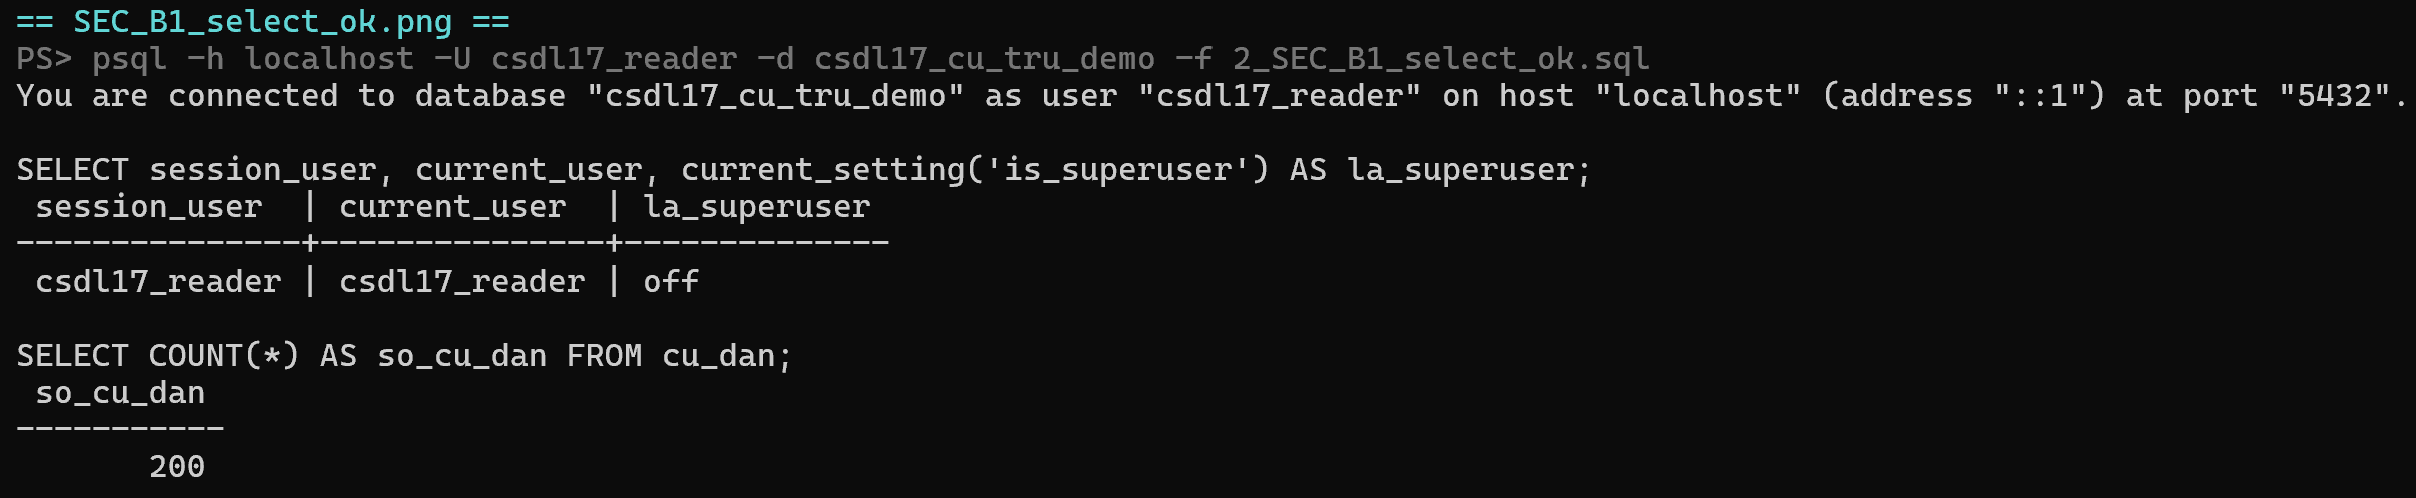
\includegraphics[trim=0bp 0bp 223bp 50bp,clip,width=\linewidth]{image/security/SEC_B1_select_ok.png}
    \caption{B1 --- Role tra cứu đăng nhập độc lập và đếm được 200 cư dân}
    \label{fig:sec-b1-select}
    \par\medskip
    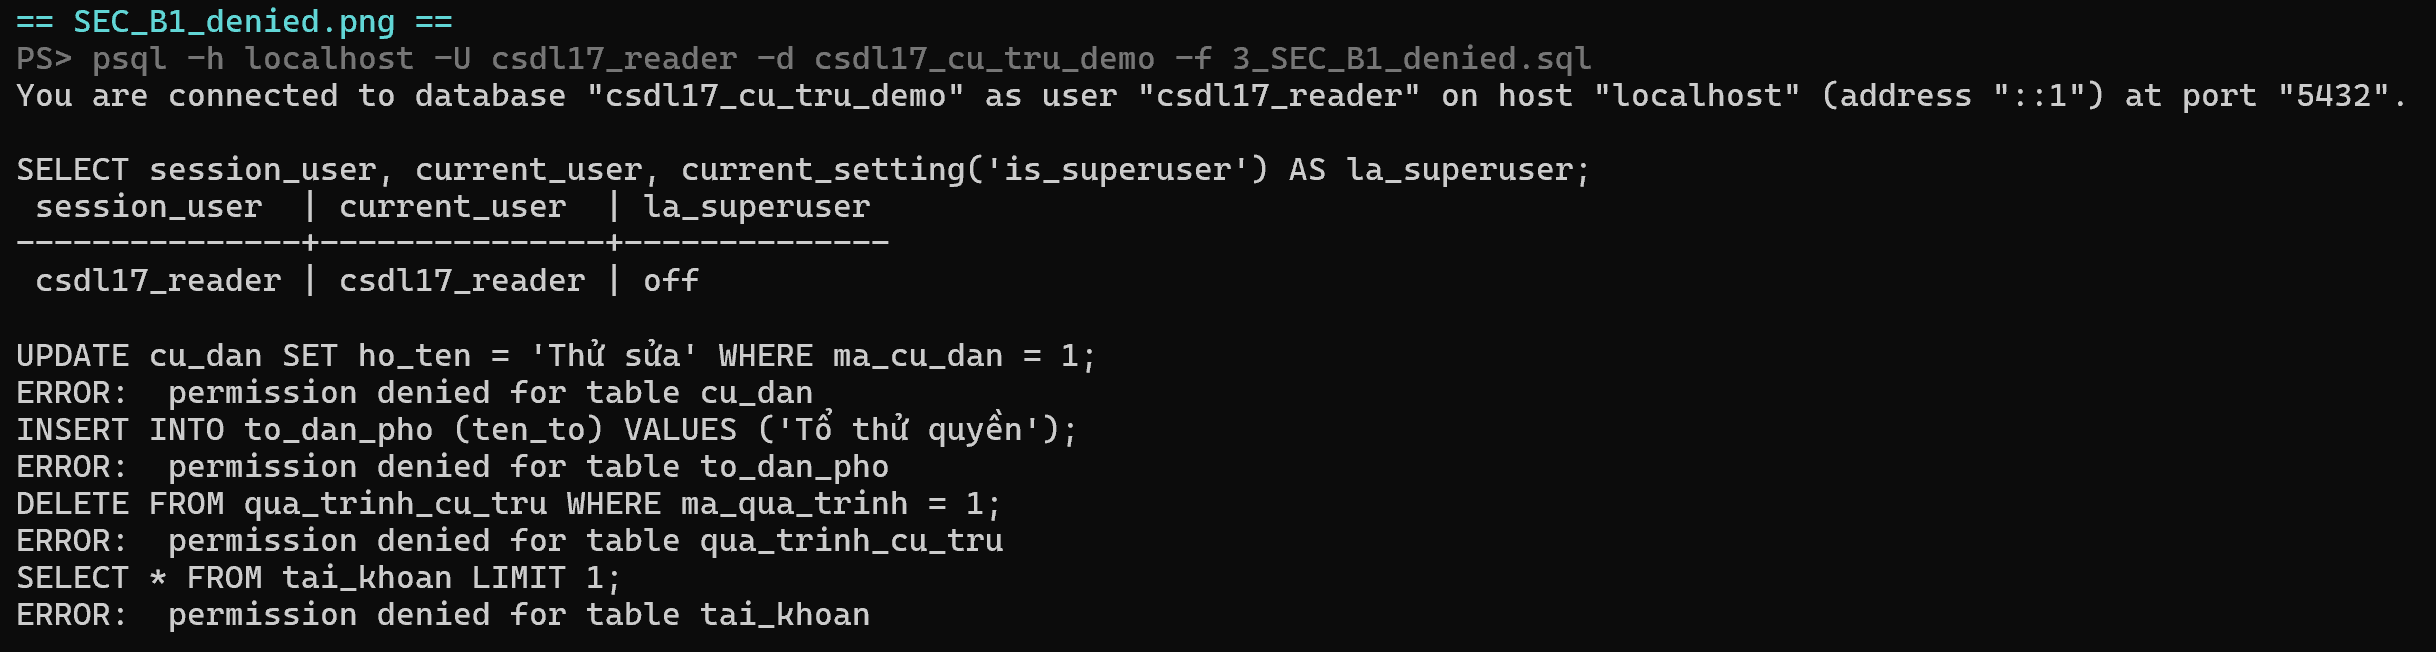
\includegraphics[trim=0bp 0bp 231bp 50bp,clip,width=\linewidth]{image/security/SEC_B1_denied.png}
    \caption{B1 --- PostgreSQL từ chối thao tác ghi và đọc bảng tài khoản}
    \label{fig:sec-b1-denied}
\end{figure}

\textbf{Ví dụ 2: Dùng khung nhìn để chỉ công bố số liệu tổng hợp (B2).} Cán bộ tổng hợp của phường cần biết mỗi tổ đang có bao nhiêu người cư trú, nhưng không cần biết họ tên hay ngày sinh của từng người. Nhóm tạo một view chỉ trả về mã tổ, tên tổ và số người, rồi chỉ cấp quyền trên view này cho role \texttt{csdl17\_report}, không cấp quyền trên bảng gốc.

\begin{lstlisting}[style=sqlvn]
CREATE ROLE csdl17_report LOGIN NOSUPERUSER NOCREATEDB NOCREATEROLE;
GRANT USAGE ON SCHEMA public TO csdl17_report;

CREATE VIEW vw_thong_ke_cu_dan_theo_to
WITH (security_invoker = false) AS
SELECT t.ma_to,
       t.ten_to,
       COUNT(DISTINCT q.ma_cu_dan) AS so_cu_dan
FROM to_dan_pho t
LEFT JOIN dia_chi d          ON d.ma_to = t.ma_to
LEFT JOIN ho_cu_tru h        ON h.ma_dia_chi = d.ma_dia_chi
LEFT JOIN qua_trinh_cu_tru q ON q.ma_ho = h.ma_ho
                            AND q.ngay_bat_dau <= CURRENT_DATE
                            AND (q.ngay_ket_thuc IS NULL
                                 OR q.ngay_ket_thuc >= CURRENT_DATE)
GROUP BY t.ma_to, t.ten_to;

GRANT SELECT ON vw_thong_ke_cu_dan_theo_to TO csdl17_report;

SET ROLE csdl17_report;
SELECT * FROM vw_thong_ke_cu_dan_theo_to ORDER BY ma_to;    -- được phép
SELECT ho_ten, ngay_sinh FROM cu_dan LIMIT 1;               -- bị từ chối
RESET ROLE;
\end{lstlisting}

Hình~\ref{fig:sec-b2-view} cho thấy \texttt{csdl17\_report} đọc được VIEW gồm ba cột và tám tổ. Trong lần chạy này, Tổ 01 có 34 cư dân và Tổ 08 có 0. PostgreSQL từ chối quyền đọc trực tiếp hai bảng gốc \texttt{cu\_dan} và \texttt{qua\_trinh\_cu\_tru} trong cùng role (Hình~\ref{fig:sec-b2-denied}). Điều này làm được nhờ tùy chọn \texttt{security\_invoker = false}: view đọc các bảng nền bằng quyền của chủ sở hữu view, nên người dùng chỉ cần quyền trên view mà không cần quyền trên từng bảng bên dưới. Khung nhìn công bố ba trường tổng hợp và ẩn các trường định danh cư dân.

\begin{figure}[H]
    \centering
    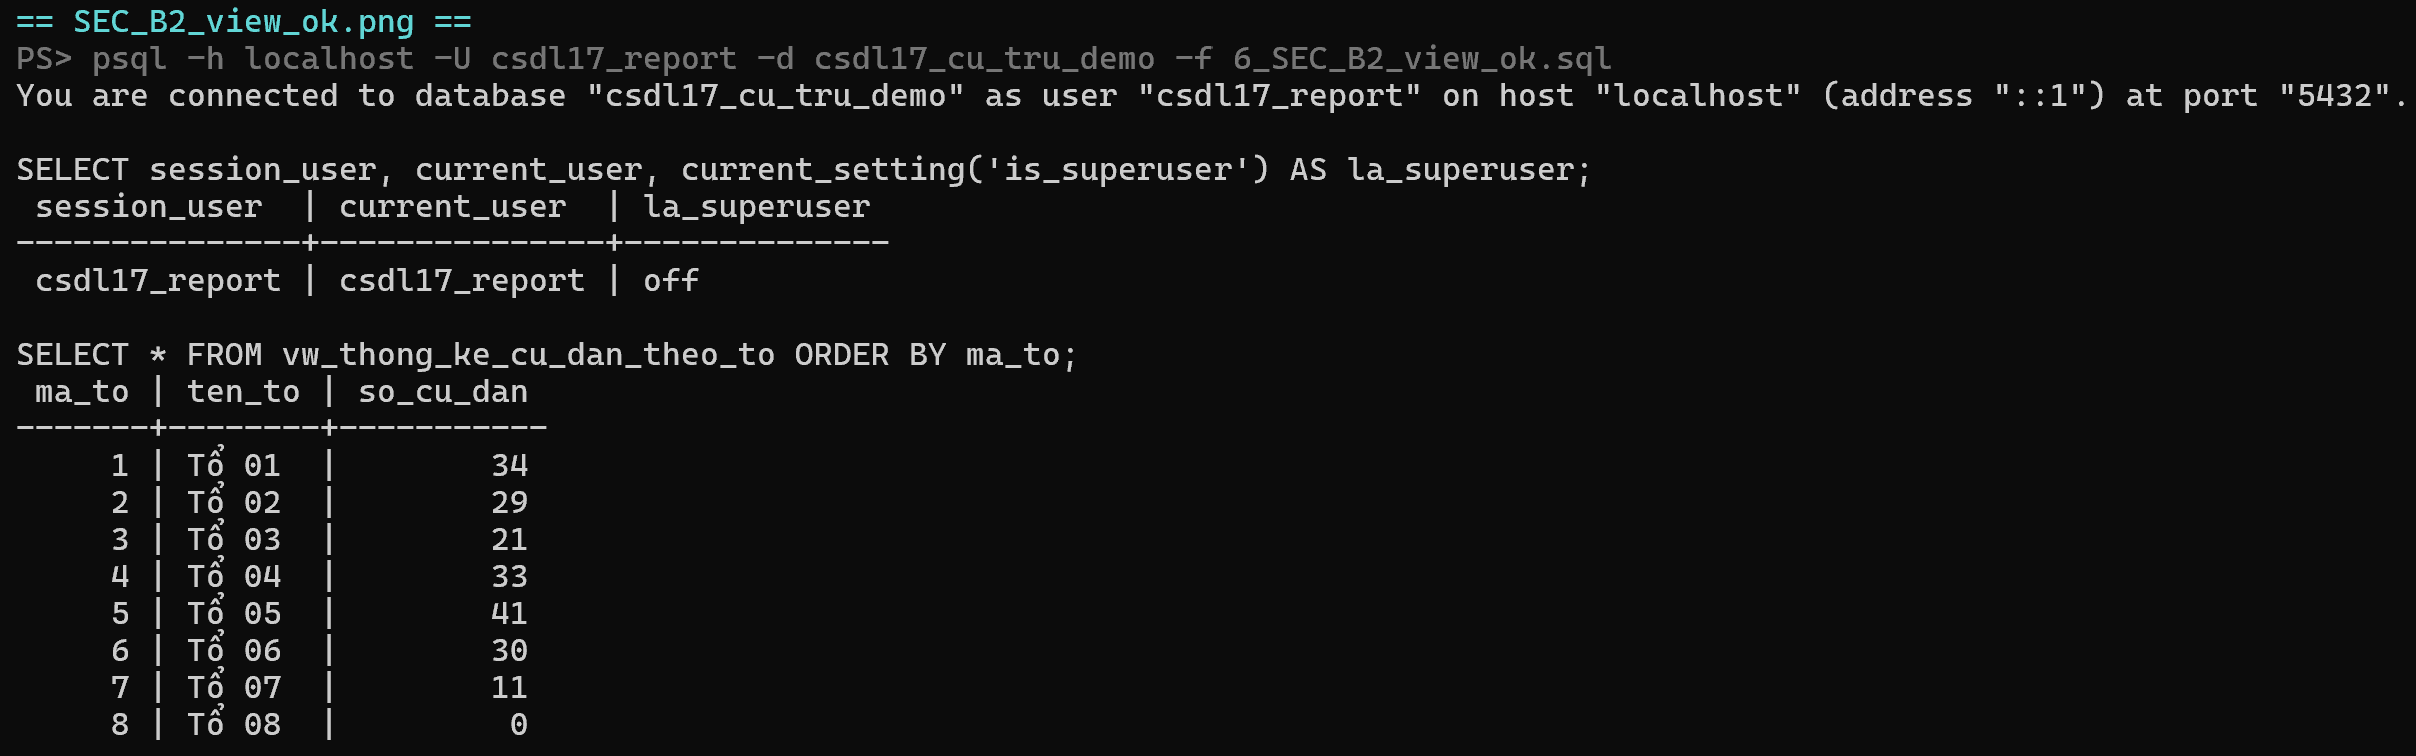
\includegraphics[trim=0bp 0bp 223bp 50bp,clip,width=\linewidth]{image/security/SEC_B2_view_ok.png}
    \caption{B2 --- Role báo cáo đăng nhập độc lập và đọc được VIEW}
    \label{fig:sec-b2-view}
    \par\medskip
    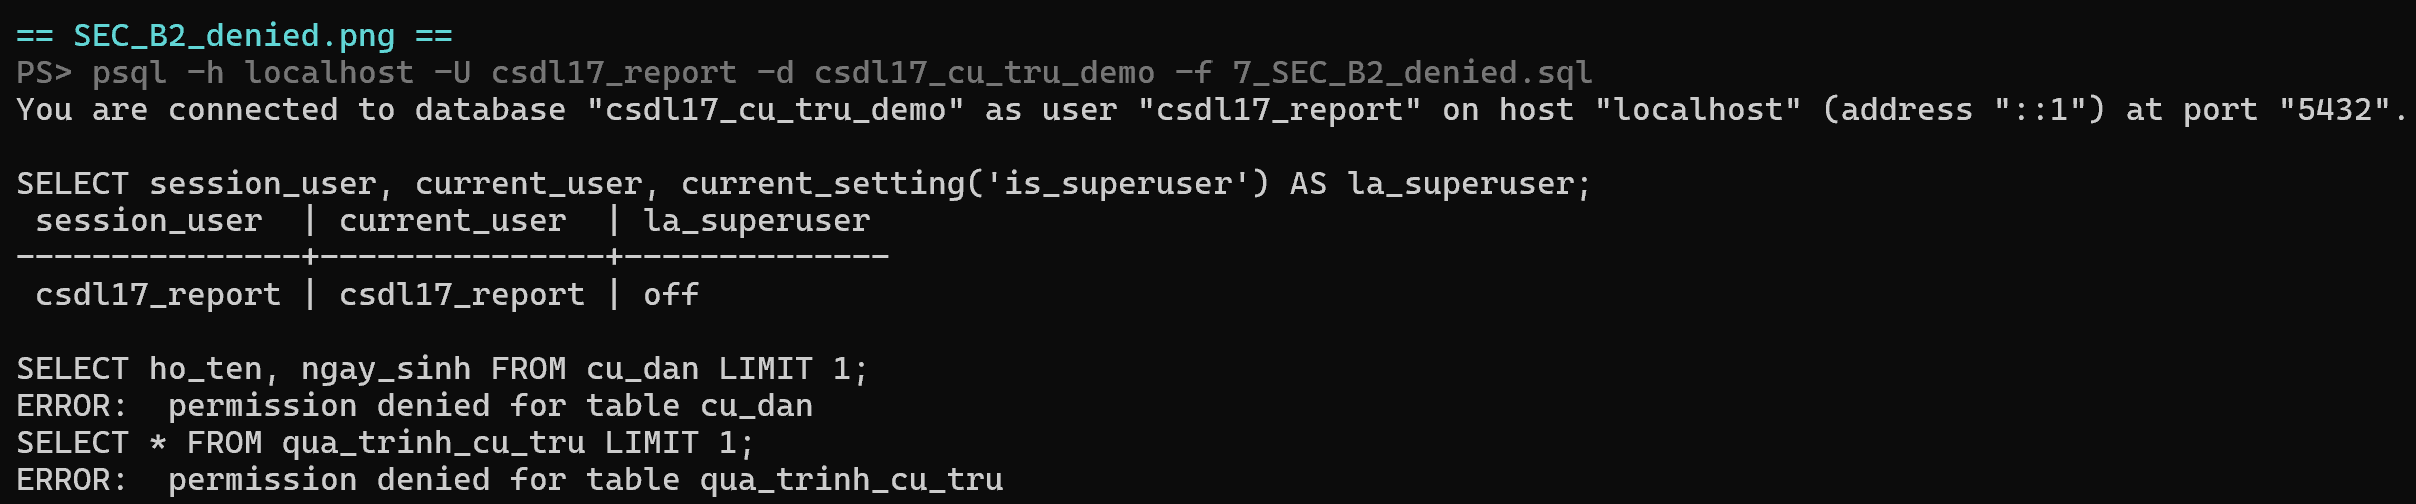
\includegraphics[trim=0bp 0bp 223bp 50bp,clip,width=\linewidth]{image/security/SEC_B2_denied.png}
    \caption{B2 --- PostgreSQL từ chối quyền đọc trực tiếp hai bảng gốc}
    \label{fig:sec-b2-denied}
\end{figure}

\textbf{Ví dụ 3: Chống tấn công SQL Injection ở chức năng tra cứu cư dân.} Chức năng tra cứu cho phép cán bộ gõ một phần họ tên để tìm cư dân. Nếu lập trình viên ghép thẳng chuỗi người dùng nhập vào một câu lệnh động như dưới đây thì kẻ xấu có thể chèn thêm mã SQL của họ.

\begin{lstlisting}[style=sqlvn]
-- CÁCH VIẾT SAI: ghép chuỗi người dùng nhập vào câu lệnh động
CREATE FUNCTION fn_tim_cu_dan_sai(p_ten TEXT)
RETURNS TABLE (ma_cu_dan BIGINT, ho_ten VARCHAR, ngay_sinh DATE)
LANGUAGE plpgsql AS $$
BEGIN
    RETURN QUERY EXECUTE
        'SELECT ma_cu_dan, ho_ten, ngay_sinh FROM cu_dan WHERE ho_ten LIKE ''%'
        || p_ten || '%''';
END;
$$;

SELECT COUNT(*) FROM fn_tim_cu_dan_sai('x'' OR 1=1 --');
-- Câu lệnh thực sự chạy là:
--   ... WHERE ho_ten LIKE '%x' OR 1=1 --%'
-- điều kiện 1=1 luôn đúng nên trả về toàn bộ 200 cư dân
\end{lstlisting}

Cách khắc phục là để giá trị người dùng nhập vào chỉ đóng vai trò tham số. Khi viết hàm bằng SQL thuần, PostgreSQL luôn coi \texttt{p\_ten} là dữ liệu cần so khớp, không bao giờ coi nó là một phần của câu lệnh. Nếu bắt buộc phải dùng câu lệnh động, cần truyền giá trị qua \texttt{EXECUTE \ldots{} USING} hoặc định dạng bằng \texttt{format('\%L', \ldots)} chứ không ghép chuỗi.

\begin{lstlisting}[style=sqlvn]
-- CÁCH VIẾT ĐÚNG: giá trị nhập vào chỉ được dùng như một tham số
CREATE FUNCTION fn_tim_cu_dan(p_ten TEXT)
RETURNS TABLE (ma_cu_dan BIGINT, ho_ten VARCHAR, ngay_sinh DATE)
LANGUAGE sql STABLE AS $$
    SELECT c.ma_cu_dan, c.ho_ten, c.ngay_sinh
    FROM cu_dan c
    WHERE c.ho_ten LIKE '%' || p_ten || '%';
$$;

REVOKE EXECUTE ON FUNCTION fn_tim_cu_dan(TEXT) FROM PUBLIC;
GRANT  EXECUTE ON FUNCTION fn_tim_cu_dan(TEXT) TO csdl17_reader;

SELECT COUNT(*) FROM fn_tim_cu_dan('x'' OR 1=1 --');   -- 0 dòng
SELECT COUNT(*) FROM fn_tim_cu_dan('Hùng');            -- 8 dòng
\end{lstlisting}

Với cùng chuỗi tấn công, hàm viết đúng chỉ tìm người có họ tên chứa đúng chuỗi ký tự đó và trả về 0 dòng, trong khi tìm theo tên ``Hùng'' vẫn ra đúng 8 cư dân. Ngoài ra, việc thu hồi quyền EXECUTE mặc định của PUBLIC rồi chỉ cấp cho csdl17\_reader cũng giúp giới hạn ai được gọi hàm tra cứu: khi chạy thử, csdl17\_reader gọi được hàm, còn csdl17\_report bị từ chối với thông báo \textit{permission denied for function fn\_tim\_cu\_dan}.

Hai hàm của Ví dụ 3 không nằm trong các script cài đặt của nhóm. Nhóm chỉ tạo chúng trên một cơ sở dữ liệu thử nghiệm riêng, trong một giao dịch kết thúc bằng ROLLBACK, để đo các con số 200, 0 và 8 ở trên; hàm viết sai chỉ dùng để minh họa lỗ hổng và không được đưa vào môi trường vận hành.

\subsection{Đánh giá kết quả và giới hạn bảo mật}
\label{subsec:danhgia}

\textbf{Kết quả kiểm thử.} Nhóm kiểm tra cấu hình quyền, thao tác được phép và thao tác bị từ chối; mỗi phép thử đối chiếu kết quả kỳ vọng với kết quả thực tế. Bảng \ref{tab:ketquabaomat} tóm tắt kết quả. Các kiểm thử đã được thực hiện trên PostgreSQL 17.11 với Windows 11 và PostgreSQL 17.12 với CSDL thử nghiệm dựng mới. Phiên đăng nhập độc lập qua TCP được kiểm tra với SCRAM-SHA-256; phép thử cục bộ không dùng mật khẩu chỉ áp dụng trong cụm tạm biệt lập. Script và log chi tiết được lưu trong hồ sơ kiểm thử của dự án.

\begin{table}[H]
\centering
\fontsize{11pt}{14pt}\selectfont
\renewcommand{\arraystretch}{1.15}
\begin{tabularx}{\textwidth}{|P{3.6cm}|Y|P{2.1cm}|}
\hline
\textbf{Kiểm thử (tệp)} & \textbf{Nội dung kiểm tra} & \textbf{Kết quả} \\
\hline
Kiểm tra quyền đã cấp (\texttt{security\_catalog\_tv3.sql}) & Ba role demo không đặc quyền, không sở hữu đối tượng, không là thành viên role khác; PUBLIC không có CONNECT/TEMP/CREATE và không có quyền trên bảng; reader chỉ đọc 6 bảng; report chỉ đọc VIEW; VIEW không có cột định danh; admin không có DELETE trên hai bảng lịch sử & 15/15 PASS \\
\hline
Đăng nhập thật bằng csdl17\_reader (\texttt{security\_login\_tv3.sql}) & SELECT được; UPDATE, INSERT, DELETE, TRUNCATE, đọc tai\_khoan, đọc VIEW, gọi \texttt{fn\_chuyen\_noi\_bo}, tạo bảng, tạo bảng tạm và SET ROLE sang admin đều bị từ chối (42501) & 12/12 PASS \\
\hline
Đăng nhập thật bằng csdl17\_report (\texttt{security\_login\_tv3.sql}) & Đọc VIEW được (8 tổ); đọc 4 bảng gốc, gọi hàm, tạo bảng, SET ROLE bị từ chối (42501); ghi VIEW báo 55000 vì VIEW có GROUP BY & 10/10 PASS \\
\hline
Bảo vệ lịch sử B12 (\texttt{security\_b12\_tv1.sql}) & Ma trận 3 role $\times$ 8 đối tượng $\times$ 5 quyền khớp thiết kế; admin DELETE, TRUNCATE hai bảng lịch sử bị từ chối; admin vẫn chạy được \texttt{fn\_chuyen\_noi\_bo} & K01--K05 PASS \\
\hline
Ví dụ của chương và quyền admin (\texttt{report\_security\_ch6.sql}) & Kết quả của Ví dụ 1--3 và các phép thử giới hạn quyền csdl17\_admin nêu dưới đây & Đúng như mô tả \\
\hline
\end{tabularx}
\caption{Tóm tắt kết quả kiểm thử bảo mật}
\label{tab:ketquabaomat}
\end{table}

Khác với \texttt{SET ROLE} ở Ví dụ 1 và 2, các phép thử đăng nhập thật mở phiên mới bằng \texttt{psql -h localhost -U csdl17\_reader} (tương tự với csdl17\_report). Dòng đầu mỗi log xác nhận \texttt{session\_user} và \texttt{current\_user} đều là role demo và phiên không phải superuser, nên kết quả phản ánh đúng quyền của role khi được dùng độc lập. Mật khẩu tạm chỉ đặt cho phiên thử và được xóa ngay sau đó, không ghi vào mã nguồn. Sau các phiên thử, giá trị băm md5 của các bảng dữ liệu không đổi. Các ảnh bổ trợ về quyền, dữ liệu trước và sau phép thử, và định nghĩa VIEW nằm trong \hyperref[sec:anh-sec]{phụ lục ảnh kiểm thử bảo mật}.

\textbf{Giới hạn của quyền csdl17\_admin.} Các phép thử trong giao dịch có \texttt{ROLLBACK} cho kết quả sau.
\begin{itemize}[leftmargin=*]
    \item \textbf{Vẫn sửa được lịch sử trong phạm vi trigger cho phép.} csdl17\_admin sửa được ghi chú của một biến động, đổi tài khoản ghi nhận của biến động cũ sang một tài khoản đang hoạt động khác, và đóng một đợt cư trú chưa gắn với biến động nào. Các lệnh làm sai quan hệ ngày giữa biến động và đợt cư trú, như đổi ngày biến động hay sửa ngày kết thúc của đợt đã gắn biến động, bị trigger B09 chặn với SQLSTATE 23514.
    \item \textbf{Quyền trên bảng tài khoản.} Role \texttt{csdl17\_admin} có quyền đọc, thêm, sửa và xóa bản ghi trên bảng \texttt{tai\_khoan}. Xóa tài khoản đã ghi biến động bị khóa ngoại chặn (23503), nhưng tài khoản chưa ghi biến động nào (tài khoản 5) thì xóa được. Admin cũng sửa được ten\_hien\_thi, vai\_tro và trang\_thai. Do nhật ký biến động chỉ lưu ma\_tai\_khoan, đổi tên hiển thị sẽ đổi cách đọc ``ai đã ghi'' của các biến động cũ; còn mở khóa một tài khoản đang KHOA thì tài khoản đó ghi lại được ngay, vì B14 chỉ kiểm tra trạng thái tại thời điểm ghi.
    \item \textbf{Vai trò nghiệp vụ chỉ là nhãn mô tả (X01, phương án b).} Cột tai\_khoan.vai\_tro chỉ là nhãn mô tả người ghi; quyền thực tế do role PostgreSQL quyết định, và trigger B14 chỉ kiểm tra tài khoản đang HOAT\_DONG chứ không kiểm tra vai trò. Bộ dữ liệu mẫu được giữ nguyên: 13/63 biến động do tài khoản có vai trò THONG\_KE ghi và 11/63 do tài khoản QUAN\_TRI ghi.
\end{itemize}

\textbf{Các giới hạn khác.} VIEW tổng hợp vẫn có nguy cơ suy luận ở nhóm nhỏ. Thống kê hiện tại dùng ngày hệ thống nên kết quả thay đổi theo thời gian. Đồ án chưa triển khai bảo mật mức dòng, kiểm toán đầy đủ, mã hóa kết nối TLS hay chính sách \texttt{pg\_hba.conf} cho vận hành. Các hàm \texttt{fn\_*} vẫn cho PUBLIC quyền EXECUTE nhưng chạy với quyền người gọi (SECURITY INVOKER); nếu đổi sang SECURITY DEFINER, phải rà soát và thu hồi quyền PUBLIC phù hợp.

\newpage
\phantomsection
\section*{KẾT LUẬN}
\addcontentsline{toc}{section}{KẾT LUẬN}
\label{sec:ketluan}

Bài tập lớn đã xây dựng cơ sở dữ liệu quản lý cư dân và biến động cư trú tại một phường trên PostgreSQL 17. Mô hình \textbf{lưu riêng các đợt cư trú theo thời gian}: mỗi đợt của một người tại một hộ có ngày bắt đầu bắt buộc và ngày kết thúc có thể để trống; mỗi biến động tham chiếu đợt cũ, đợt mới hoặc cả hai tùy loại sự kiện, đồng thời ghi tài khoản và thời điểm nhập. Thiết kế hỗ trợ tra cứu lịch sử đã ghi nhận, còn việc bảo vệ các bản ghi phụ thuộc quyền và trigger. Kết quả cụ thể của nhóm như sau.

\begin{enumerate}[leftmargin=*]
    \item \textbf{Thiết kế dữ liệu.} Từ bài toán và 14 chức năng cấp 2, nhóm xây dựng mô hình thực thể liên kết theo ký hiệu Chen rồi ánh xạ sang 7 bảng với 35 cột, 7 khóa chính, 7 khóa ngoại và 5 ràng buộc UNIQUE; hai UNIQUE trên cột đợt cũ và đợt mới thể hiện hai liên kết 1 -- 1 giữa đợt cư trú và biến động. Thực thể Quá trình cư trú giải quan hệ nhiều -- nhiều giữa cư dân và hộ, đồng thời là nguồn dữ liệu tham chiếu để tra cứu các đợt đã lưu theo mã cư dân. Kết quả phân tích BCNF theo tập phụ thuộc hàm đã xét được nêu ở mục \ref{subsec:chuanhoa}. Ngày biến động trùng với ngày của đợt là dữ liệu lặp giữa hai bảng, được trigger B09 giữ cho khớp.
    \item \textbf{Ràng buộc nghiệp vụ.} Ngoài khóa và CHECK, các quy tắc B06 -- B15 được cài bằng ràng buộc loại trừ GiST (không chồng lấn đợt cùng loại), trigger kiểm tra hình dạng và ngày của biến động, trigger giữ địa chỉ đã có lịch sử, ba hàm chuyển nội bộ, chuyển đi và chuyển đến thực hiện trong một giao dịch, và trigger kiểm tra ngày hợp lý. Cơ sở dữ liệu dựng mới nạp được bộ dữ liệu kiểm thử gồm 636 bản ghi, bước kiểm tra dữ liệu không phát hiện vi phạm, và các câu lệnh cố tình vi phạm đều bị từ chối với đúng mã lỗi.
    \item \textbf{Truy vấn.} Báo cáo trình bày 10 câu đại số quan hệ, gồm đủ phép chọn, chiếu, kết nối theo điều kiện, đổi tên, hợp, giao, hiệu, chia và phép gom nhóm của đại số quan hệ mở rộng, cùng 13 câu SQL dùng kết nối nhiều bảng, kết nối ngoài, gom nhóm có HAVING, truy vấn con tương quan, truy vấn con trong FROM, CTE, hàm cửa sổ RANK() và phép chia viết bằng hai lớp NOT EXISTS. Kết quả của cả 13 câu QSQL khớp với dữ liệu đối chiếu khi chạy lại trên cơ sở dữ liệu dựng mới. Các biểu thức đại số quan hệ được kiểm chứng bằng những truy vấn SQL đối chứng tương ứng.
    \item \textbf{Bảo mật.} Hai ví dụ kiểm thử quyền dùng phân quyền theo nguyên tắc quyền tối thiểu (role chỉ đọc bị từ chối khi sửa dữ liệu, role quản trị không xóa được lịch sử) và khung nhìn chỉ công bố số liệu tổng hợp theo tổ. Cả hai đã được kiểm tra bằng phiên đăng nhập thật của từng role và bằng cách kiểm tra quyền đã cấp. Ví dụ SQL Injection minh họa vì sao phải truyền dữ liệu người dùng như tham số thay vì ghép chuỗi vào câu lệnh động.
\end{enumerate}

Cột vai trò của tài khoản chỉ là nhãn nghiệp vụ, không ngăn tài khoản thống kê ghi biến động (X01). B15 chưa kiểm tra được ngày sinh hay ngày lập hộ ở tương lai khi chưa có đợt cư trú (X06). B10 chỉ được bảo đảm khi ghi biến động qua ba hàm chuyển; role quản trị vẫn sửa trực tiếp được bảng đợt cư trú, nên vẫn có thể đóng một đợt mà không ghi biến động. Role quản trị vẫn có quyền sửa hai bảng lịch sử trong phạm vi trigger cho phép và có quyền đọc, thêm, sửa và xóa bản ghi trên bảng tài khoản, nên có thể đổi người ghi của biến động cũ, đổi tên hiển thị hoặc mở khóa tài khoản. Đồ án cũng chưa triển khai bảo mật mức dòng, nhật ký kiểm toán đầy đủ và mã hóa kết nối.

Về nghiệp vụ, mô hình còn đơn giản hơn thực tế quản lý cư trú ở bốn điểm. Thứ nhất, cư dân chưa có số định danh cá nhân (số CCCD) và họ tên được phép trùng, nên không phân biệt được hai người trùng cả họ tên lẫn ngày sinh ngoài mã cư dân do hệ thống cấp. Thứ hai, hộ chưa có chủ hộ và chưa lưu quan hệ của từng thành viên với chủ hộ. Thứ ba, việc đổi từ tạm trú sang thường trú trong cùng một hộ chưa được ghi thành biến động, vì CHUYEN\_NOI\_BO bắt buộc hai hộ khác nhau (B08). Thứ tư, chưa có loại biến động cho khai sinh và khai tử; hiện tại người mới sinh chỉ có thể được ghi như chuyển đến, còn người mất như chuyển đi. Nhóm triển khai cơ sở dữ liệu trong môi trường kiểm thử và dùng bộ dữ liệu tự tạo để ghi nhận các kết quả trong báo cáo.

Trong thời gian tới, cơ sở dữ liệu có thể được hoàn thiện theo các hướng: bổ sung số định danh cá nhân có ràng buộc UNIQUE cho cư dân, chủ hộ và quan hệ với chủ hộ, cùng các loại biến động đổi loại cư trú, khai sinh và khai tử; chỉ cho ghi biến động qua các hàm chuyển; thu hẹp quyền của role quản trị trên bảng tài khoản và cột người ghi của biến động, bổ sung bảng nhật ký kiểm toán ghi lại mọi lệnh sửa dữ liệu lịch sử; ràng buộc vai trò được phép ghi biến động nếu nghiệp vụ yêu cầu; áp dụng bảo mật mức dòng để mỗi cán bộ chỉ xem dữ liệu của tổ mình; và bổ sung chức năng thống kê lịch sử theo nhu cầu tra cứu.

\renewcommand{\refname}{Tài liệu tham khảo}
\phantomsection
\addcontentsline{toc}{section}{Tài liệu tham khảo}
\begin{thebibliography}{99}
\raggedright
\interlinepenalty=10000

\bibitem{elmasri}
R. Elmasri và S. B. Navathe, \textit{Fundamentals of Database Systems}, ấn bản 7, Pearson, 2016.

\bibitem{silberschatz}
A. Silberschatz, H. F. Korth và S. Sudarshan, \textit{Database System Concepts}, ấn bản 7, McGraw-Hill, 2020.

\bibitem{postgres}
The PostgreSQL Global Development Group, \textit{PostgreSQL 17 Documentation}. [Trực tuyến]. Có tại: \url{https://www.postgresql.org/docs/17/}.

\bibitem{pgidentity}
The PostgreSQL Global Development Group, \textit{PostgreSQL 17 Documentation: Identity Columns}. [Trực tuyến]. Có tại: \url{https://www.postgresql.org/docs/17/ddl-identity-columns.html}.

\bibitem{pgexpressionindex}
The PostgreSQL Global Development Group, \textit{PostgreSQL 17 Documentation: Indexes on Expressions}. [Trực tuyến]. Có tại: \url{https://www.postgresql.org/docs/17/indexes-expressional.html}.

\bibitem{luat91}
Quốc hội nước Cộng hòa xã hội chủ nghĩa Việt Nam, \textit{Luật Bảo vệ dữ liệu cá nhân}, số 91/2025/QH15, thông qua ngày 26/6/2025 tại kỳ họp thứ 9, Quốc hội khóa XV; có hiệu lực từ ngày 01/01/2026 (Điều 38). [Trực tuyến]. Có tại: \url{https://vanban.chinhphu.vn/?pageid=27160&docid=214590}.

\bibitem{nd356}
Chính phủ nước Cộng hòa xã hội chủ nghĩa Việt Nam, \textit{Nghị định số 356/2025/NĐ-CP quy định chi tiết một số điều và biện pháp thi hành Luật Bảo vệ dữ liệu cá nhân}, ban hành ngày 31/12/2025; có hiệu lực từ ngày 01/01/2026, đồng thời Nghị định số 13/2023/NĐ-CP ngày 17/4/2023 hết hiệu lực (Điều 42). [Trực tuyến]. Có tại: \url{https://chinhphu.vn/?docid=216387&pageid=27160}.

\end{thebibliography}

\newpage
\phantomsection
\section*{PHỤ LỤC A. MÃ NGUỒN TRIGGER VÀ HÀM}
\addcontentsline{toc}{section}{Phụ lục A. Mã nguồn trigger và hàm}
\label{sec:phuluc}

Phụ lục này chép nguyên văn các trigger và hàm trong tệp \texttt{sql/02\_constraints.sql} đã nhắc tới ở mục \ref{subsec:rangbuoc}. Mỗi đoạn mã có vài dòng giải thích ngắn ở phía trên. Các trigger đều báo lỗi với mã SQLSTATE 23514 (vi phạm ràng buộc kiểm tra) hoặc 23503 (tham chiếu tới dòng không tồn tại), giống như các ràng buộc có sẵn của PostgreSQL.

\subsection*{A.1. Hàm kiểm tra một biến động (B08, B09)}
\addcontentsline{toc}{subsection}{A.1. Hàm kiểm tra một biến động (B08, B09)}

Hàm \texttt{fn\_kiem\_tra\_su\_kien} chứa toàn bộ phần kiểm tra B08 và B09, được hai trigger ở mục A.2 và A.3 gọi lại. Hàm kiểm tra đợt cũ phải kết thúc đúng một ngày trước ngày chuyển, đợt mới phải bắt đầu đúng ngày chuyển, và với chuyển nội bộ thì hai đợt phải cùng cư dân nhưng khác hộ. Lệnh \texttt{FOR SHARE} khóa tạm các đợt đang đọc để một giao dịch khác không sửa chúng giữa chừng.

\begin{lstlisting}[style=sqlvn, caption={Hàm kiểm tra một biến động (B08, B09)}, label={lst:pl_kiemtra}]
-- B08/B09: kiểm tra đầy đủ một sự kiện, có khóa SHARE để đồng bộ
-- với thao tác UPDATE đợt cư trú chạy đồng thời.
CREATE OR REPLACE FUNCTION fn_kiem_tra_su_kien(
    p_loai VARCHAR, p_cu BIGINT, p_moi BIGINT, p_ngay DATE
) RETURNS void LANGUAGE plpgsql AS $fn$
DECLARE
    v_cu qua_trinh_cu_tru%ROWTYPE;
    v_moi qua_trinh_cu_tru%ROWTYPE;
BEGIN
    -- CHECK gốc chạy sau BEFORE trigger: giữ mã lỗi nhất quán cho dạng thiếu FK.
    IF p_loai = 'CHUYEN_NOI_BO' AND (p_cu IS NULL OR p_moi IS NULL) THEN
        RAISE EXCEPTION 'B08: chuyển nội bộ phải có cả đợt cũ và mới'
            USING ERRCODE = '23514';
    END IF;

    IF p_cu IS NOT NULL THEN
        SELECT * INTO v_cu FROM qua_trinh_cu_tru
        WHERE ma_qua_trinh = p_cu FOR SHARE;
        IF NOT FOUND THEN
            RAISE EXCEPTION 'B09: đợt cũ % không tồn tại', p_cu
                USING ERRCODE = '23503';
        END IF;
        IF v_cu.ngay_ket_thuc IS DISTINCT FROM (p_ngay - 1) THEN
            RAISE EXCEPTION 'B09: đợt cũ % phải kết thúc trước ngày chuyển % đúng 1 ngày',
                p_cu, p_ngay USING ERRCODE = '23514';
        END IF;
    END IF;

    IF p_moi IS NOT NULL THEN
        SELECT * INTO v_moi FROM qua_trinh_cu_tru
        WHERE ma_qua_trinh = p_moi FOR SHARE;
        IF NOT FOUND THEN
            RAISE EXCEPTION 'B09: đợt mới % không tồn tại', p_moi
                USING ERRCODE = '23503';
        END IF;
        IF v_moi.ngay_bat_dau IS DISTINCT FROM p_ngay THEN
            RAISE EXCEPTION 'B09: đợt mới % phải bắt đầu đúng ngày chuyển %',
                p_moi, p_ngay USING ERRCODE = '23514';
        END IF;
    END IF;

    IF p_loai = 'CHUYEN_NOI_BO' THEN
        IF v_cu.ma_cu_dan IS DISTINCT FROM v_moi.ma_cu_dan
           OR v_cu.ma_ho IS NOT DISTINCT FROM v_moi.ma_ho THEN
            RAISE EXCEPTION 'B08: chuyển nội bộ phải cùng cư dân, khác hộ'
                USING ERRCODE = '23514';
        END IF;
    END IF;
END
$fn$;
\end{lstlisting}

\subsection*{A.2. Trigger khi ghi biến động: B08, B09 chiều thuận và B14}
\addcontentsline{toc}{subsection}{A.2. Trigger khi ghi biến động: B08, B09 chiều thuận và B14}

Trigger \texttt{trg\_bien\_dong\_hop\_le} chạy trước mỗi lệnh thêm hoặc sửa biến động. Khi thêm mới hoặc đổi người ghi, trigger kiểm tra tài khoản phải đang ở trạng thái HOAT\_DONG (B14); sau đó gọi hàm ở mục A.1 để kiểm tra ngày và hai đợt cư trú của biến động.

\begin{lstlisting}[style=sqlvn, caption={Trigger khi ghi biến động: B08, B09 chiều thuận và B14}, label={lst:pl_bd}]
-- B14: lúc ghi sự kiện hoặc đổi người ghi phải dùng tài khoản HOAT_DONG.
-- Khóa tài khoản về sau không làm vô hiệu sự kiện lịch sử.
CREATE OR REPLACE FUNCTION fn_truoc_ghi_bien_dong()
RETURNS trigger LANGUAGE plpgsql AS $fn$
DECLARE
    v_kiem_tra_tai_khoan BOOLEAN := FALSE;
    v_trang_thai VARCHAR(20);
BEGIN
    IF TG_OP = 'INSERT' THEN
        v_kiem_tra_tai_khoan := TRUE;
    ELSIF NEW.ma_tai_khoan IS DISTINCT FROM OLD.ma_tai_khoan THEN
        v_kiem_tra_tai_khoan := TRUE;
    END IF;

    IF v_kiem_tra_tai_khoan THEN
        SELECT trang_thai INTO v_trang_thai FROM tai_khoan
        WHERE ma_tai_khoan = NEW.ma_tai_khoan FOR SHARE;
        IF v_trang_thai IS DISTINCT FROM 'HOAT_DONG' THEN
            RAISE EXCEPTION 'B14: tài khoản % không ở trạng thái HOAT_DONG', NEW.ma_tai_khoan
                USING ERRCODE = '23514';
        END IF;
    END IF;

    PERFORM fn_kiem_tra_su_kien(
        NEW.loai_bien_dong, NEW.ma_qua_trinh_cu,
        NEW.ma_qua_trinh_moi, NEW.ngay_bien_dong
    );
    RETURN NEW;
END
$fn$;

DROP TRIGGER IF EXISTS trg_bien_dong_hop_le ON bien_dong_cu_tru;
CREATE TRIGGER trg_bien_dong_hop_le
BEFORE INSERT OR UPDATE ON bien_dong_cu_tru
FOR EACH ROW EXECUTE FUNCTION fn_truoc_ghi_bien_dong();
\end{lstlisting}

\subsection*{A.3. Trigger khi sửa đợt cư trú: B08, B09 chiều ngược}
\addcontentsline{toc}{subsection}{A.3. Trigger khi sửa đợt cư trú: B08, B09 chiều ngược}

Đây là chiều ngược của mục A.2: khi sửa cư dân, hộ hoặc ngày của một đợt đã có, trigger \texttt{trg\_dot\_khong\_pha\_su\_kien} kiểm tra lại mọi biến động đang trỏ tới đợt đó. Nhờ vậy không thể sửa ngày của đợt làm sai một biến động đã ghi từ trước.

\begin{lstlisting}[style=sqlvn, caption={Trigger khi sửa đợt cư trú: B08, B09 chiều ngược}, label={lst:pl_dot}]
-- B08/B09 chiều ngược: sửa một đợt không được làm hỏng sự kiện cũ.
CREATE OR REPLACE FUNCTION fn_sau_sua_dot_cu_tru()
RETURNS trigger LANGUAGE plpgsql AS $fn$
DECLARE
    v_su_kien bien_dong_cu_tru%ROWTYPE;
BEGIN
    IF (NEW.ma_cu_dan, NEW.ma_ho, NEW.ngay_bat_dau, NEW.ngay_ket_thuc)
       IS DISTINCT FROM
       (OLD.ma_cu_dan, OLD.ma_ho, OLD.ngay_bat_dau, OLD.ngay_ket_thuc) THEN
        FOR v_su_kien IN
            SELECT * FROM bien_dong_cu_tru
            WHERE ma_qua_trinh_cu = NEW.ma_qua_trinh
               OR ma_qua_trinh_moi = NEW.ma_qua_trinh
        LOOP
            PERFORM fn_kiem_tra_su_kien(
                v_su_kien.loai_bien_dong,
                v_su_kien.ma_qua_trinh_cu,
                v_su_kien.ma_qua_trinh_moi,
                v_su_kien.ngay_bien_dong
            );
        END LOOP;
    END IF;
    RETURN NEW;
END
$fn$;

DROP TRIGGER IF EXISTS trg_dot_khong_pha_su_kien ON qua_trinh_cu_tru;
CREATE TRIGGER trg_dot_khong_pha_su_kien
AFTER UPDATE OF ma_cu_dan, ma_ho, ngay_bat_dau, ngay_ket_thuc
ON qua_trinh_cu_tru
FOR EACH ROW EXECUTE FUNCTION fn_sau_sua_dot_cu_tru();
\end{lstlisting}

\subsection*{A.4. Trigger giữ địa chỉ của lịch sử (B11)}
\addcontentsline{toc}{subsection}{A.4. Trigger giữ địa chỉ của lịch sử (B11)}

Một hàm dùng chung cho hai trigger: không cho đổi địa chỉ của một hộ, và không cho đổi tổ của một địa chỉ, khi đã có đợt cư trú gắn với hộ hoặc địa chỉ đó. Biến \texttt{TG\_TABLE\_NAME} cho biết trigger đang chạy trên bảng nào để chọn phép kiểm tra phù hợp.

\begin{lstlisting}[style=sqlvn, caption={Trigger giữ địa chỉ của lịch sử (B11)}, label={lst:pl_b11}]
-- B11: không chuyển địa chỉ/tổ "ngầm" trên lịch sử đã có.
CREATE OR REPLACE FUNCTION fn_khoa_dia_chi_lich_su()
RETURNS trigger LANGUAGE plpgsql AS $fn$
BEGIN
    IF TG_TABLE_NAME = 'ho_cu_tru' THEN
        IF NEW.ma_dia_chi IS DISTINCT FROM OLD.ma_dia_chi
           AND EXISTS (SELECT 1 FROM qua_trinh_cu_tru WHERE ma_ho = OLD.ma_ho) THEN
            RAISE EXCEPTION 'B11: không đổi địa chỉ của hộ % đã có lịch sử', OLD.ma_ho
                USING ERRCODE = '23514';
        END IF;
    ELSIF TG_TABLE_NAME = 'dia_chi' THEN
        IF NEW.ma_to IS DISTINCT FROM OLD.ma_to
           AND EXISTS (
               SELECT 1 FROM ho_cu_tru h
               JOIN qua_trinh_cu_tru q ON q.ma_ho = h.ma_ho
               WHERE h.ma_dia_chi = OLD.ma_dia_chi
           ) THEN
            RAISE EXCEPTION 'B11: không đổi tổ của địa chỉ % đã có lịch sử', OLD.ma_dia_chi
                USING ERRCODE = '23514';
        END IF;
    END IF;
    RETURN NEW;
END
$fn$;

DROP TRIGGER IF EXISTS trg_ho_giu_dia_chi_lich_su ON ho_cu_tru;
CREATE TRIGGER trg_ho_giu_dia_chi_lich_su
BEFORE UPDATE OF ma_dia_chi ON ho_cu_tru
FOR EACH ROW EXECUTE FUNCTION fn_khoa_dia_chi_lich_su();

DROP TRIGGER IF EXISTS trg_dia_chi_giu_to_lich_su ON dia_chi;
CREATE TRIGGER trg_dia_chi_giu_to_lich_su
BEFORE UPDATE OF ma_to ON dia_chi
FOR EACH ROW EXECUTE FUNCTION fn_khoa_dia_chi_lich_su();
\end{lstlisting}

\subsection*{A.5. Trigger kiểm tra ngày hợp lý (B15)}
\addcontentsline{toc}{subsection}{A.5. Trigger kiểm tra ngày hợp lý (B15)}

Phần này kiểm tra ngày sinh của cư dân và ngày lập hộ không được muộn hơn ngày bắt đầu đợt cư trú. Hàm thứ nhất chạy khi thêm hoặc sửa đợt cư trú; hàm thứ hai chạy khi sửa ngày sinh hoặc ngày lập hộ, tức là kiểm tra theo cả hai chiều. Năm ràng buộc CHECK của B15 về tên không rỗng đã nêu ở mục \ref{subsec:rangbuoc} nên không chép lại.

\begin{lstlisting}[style=sqlvn, caption={Trigger kiểm tra ngày hợp lý (B15)}, label={lst:pl_b15}]
-- B15: kiểm tra cả chiều INSERT/UPDATE đợt và sửa hồ sơ cha.
CREATE OR REPLACE FUNCTION fn_b15_kiem_tra_dot()
RETURNS trigger LANGUAGE plpgsql AS $fn$
DECLARE
    v_ngay_sinh DATE;
    v_ngay_lap DATE;
BEGIN
    SELECT ngay_sinh INTO v_ngay_sinh FROM cu_dan
    WHERE ma_cu_dan = NEW.ma_cu_dan FOR SHARE;
    SELECT ngay_lap INTO v_ngay_lap FROM ho_cu_tru
    WHERE ma_ho = NEW.ma_ho FOR SHARE;

    -- FK còn bảo vệ trường hợp mã cư dân / mã hộ không tồn tại.
    IF v_ngay_sinh > NEW.ngay_bat_dau
       OR v_ngay_lap > NEW.ngay_bat_dau THEN
        RAISE EXCEPTION 'B15: ngày sinh hoặc ngày lập hộ sau ngày bắt đầu cư trú'
            USING ERRCODE = '23514';
    END IF;
    RETURN NEW;
END
$fn$;

DROP TRIGGER IF EXISTS trg_b15_dot ON qua_trinh_cu_tru;
CREATE TRIGGER trg_b15_dot
BEFORE INSERT OR UPDATE OF ma_cu_dan, ma_ho, ngay_bat_dau
ON qua_trinh_cu_tru
FOR EACH ROW EXECUTE FUNCTION fn_b15_kiem_tra_dot();

CREATE OR REPLACE FUNCTION fn_b15_kiem_tra_cha()
RETURNS trigger LANGUAGE plpgsql AS $fn$
BEGIN
    IF TG_TABLE_NAME = 'cu_dan' THEN
        IF EXISTS (
            SELECT 1 FROM qua_trinh_cu_tru
            WHERE ma_cu_dan = NEW.ma_cu_dan
              AND ngay_bat_dau < NEW.ngay_sinh
        ) THEN
            RAISE EXCEPTION 'B15: sửa ngày sinh mâu thuẫn lịch sử cư trú'
                USING ERRCODE = '23514';
        END IF;
    ELSIF TG_TABLE_NAME = 'ho_cu_tru' THEN
        IF EXISTS (
            SELECT 1 FROM qua_trinh_cu_tru
            WHERE ma_ho = NEW.ma_ho
              AND ngay_bat_dau < NEW.ngay_lap
        ) THEN
            RAISE EXCEPTION 'B15: sửa ngày lập hộ mâu thuẫn lịch sử cư trú'
                USING ERRCODE = '23514';
        END IF;
    END IF;
    RETURN NEW;
END
$fn$;

DROP TRIGGER IF EXISTS trg_b15_ngay_sinh ON cu_dan;
CREATE TRIGGER trg_b15_ngay_sinh
BEFORE UPDATE OF ngay_sinh ON cu_dan
FOR EACH ROW EXECUTE FUNCTION fn_b15_kiem_tra_cha();

DROP TRIGGER IF EXISTS trg_b15_ngay_lap_ho ON ho_cu_tru;
CREATE TRIGGER trg_b15_ngay_lap_ho
BEFORE UPDATE OF ngay_lap ON ho_cu_tru
FOR EACH ROW EXECUTE FUNCTION fn_b15_kiem_tra_cha();
\end{lstlisting}

\subsection*{A.6. Hàm chuyển nội bộ trong một giao dịch (B10)}
\addcontentsline{toc}{subsection}{A.6. Hàm chuyển nội bộ trong một giao dịch (B10)}

Hàm \texttt{fn\_chuyen\_noi\_bo} gộp ba bước của một lần chuyển nội bộ: kết thúc đợt cũ vào ngày trước ngày chuyển, mở đợt mới ở hộ mới và ghi biến động. Cả ba bước nằm trong cùng một lần gọi hàm, nên nếu một bước lỗi thì cả ba đều bị hủy. Lệnh \texttt{FOR UPDATE} khóa đợt cũ để hai cán bộ không chuyển cùng một người cùng lúc.

\begin{lstlisting}[style=sqlvn, caption={Hàm chuyển nội bộ trong một giao dịch (B10)}, label={lst:pl_chuyen}]
-- B10: một lần gọi hàm được PostgreSQL thực hiện nguyên tử;
-- luôn đặt trong transaction bên ngoài để gom các bước nghiệp vụ khác.
-- Mở/đóng đợt và ghi sự kiện cùng giao dịch, khóa đợt cũ FOR UPDATE.
-- Không thay đổi loại cư trú đợt cũ; loại đợt mới được truyền vào.
CREATE OR REPLACE FUNCTION fn_chuyen_noi_bo(
    p_ma_qua_trinh_cu BIGINT,
    p_ma_ho_moi BIGINT,
    p_loai_moi VARCHAR(20),
    p_ngay_chuyen DATE,
    p_ma_tai_khoan BIGINT
) RETURNS TABLE(ma_dot_moi BIGINT, ma_su_kien BIGINT)
LANGUAGE plpgsql AS $fn$
DECLARE
    v_cu qua_trinh_cu_tru%ROWTYPE;
    v_moi BIGINT;
    v_sk BIGINT;
BEGIN
    SELECT * INTO v_cu FROM qua_trinh_cu_tru
    WHERE ma_qua_trinh = p_ma_qua_trinh_cu FOR UPDATE;
    IF NOT FOUND THEN
        RAISE EXCEPTION 'B10: đợt cũ % không tồn tại', p_ma_qua_trinh_cu
            USING ERRCODE = '23503';
    END IF;
    IF v_cu.ngay_ket_thuc IS NOT NULL OR p_ngay_chuyen <= v_cu.ngay_bat_dau THEN
        RAISE EXCEPTION 'B10: đợt cũ phải đang mở và bắt đầu trước ngày chuyển'
            USING ERRCODE = '23514';
    END IF;
    IF p_ma_ho_moi = v_cu.ma_ho THEN
        RAISE EXCEPTION 'B08: hộ mới phải khác hộ cũ'
            USING ERRCODE = '23514';
    END IF;

    UPDATE qua_trinh_cu_tru
    SET ngay_ket_thuc = p_ngay_chuyen - 1
    WHERE ma_qua_trinh = p_ma_qua_trinh_cu;

    INSERT INTO qua_trinh_cu_tru (
        ma_cu_dan, ma_ho, loai_cu_tru, ngay_bat_dau, ngay_ket_thuc
    ) VALUES (v_cu.ma_cu_dan, p_ma_ho_moi, p_loai_moi, p_ngay_chuyen, NULL)
    RETURNING ma_qua_trinh INTO v_moi;

    INSERT INTO bien_dong_cu_tru (
        loai_bien_dong, ma_qua_trinh_cu, ma_qua_trinh_moi,
        ngay_bien_dong, ma_tai_khoan
    ) VALUES (
        'CHUYEN_NOI_BO', p_ma_qua_trinh_cu, v_moi,
        p_ngay_chuyen, p_ma_tai_khoan
    ) RETURNING ma_bien_dong INTO v_sk;

    RETURN QUERY SELECT v_moi, v_sk;
END
$fn$;
\end{lstlisting}

\clearpage
\phantomsection
\section*{PHỤ LỤC B. BẢNG TRA MÃ QUY TẮC VÀ KIỂM THỬ}
\addcontentsline{toc}{section}{Phụ lục B. Bảng tra mã quy tắc và kiểm thử}
\label{sec:phuluc-ma}

Phụ lục liệt kê đủ các mã được nhắc tới trong báo cáo. Mã B là quy tắc nghiệp vụ trong đặc tả; E1 là điều kiện kiểm tra dữ liệu; mã X là giới hạn đã biết, được nhóm ghi nhận khi rà soát thiết kế; mã K là các ca kiểm thử quyền của role quản trị. Riêng ``Demo B1'' và ``Demo B2'' ở Chương 6 là tên hai ví dụ bảo mật, không phải quy tắc B01 hay B02. Cột cuối cho biết quy tắc được bảo đảm ở đâu hoặc được nhắc tới ở đâu.

{\fontsize{11pt}{13pt}\selectfont
\renewcommand{\arraystretch}{1.10}
\begin{longtable}{@{}P{1.15cm}P{8.5cm}P{4.4cm}@{}}
\caption{Quy tắc nghiệp vụ B01--B18}\label{tab:mab}\\
\hline
\rowcolor{black!7}
\textbf{Mã} & \textbf{Nội dung} & \textbf{Cách bảo đảm} \\
\hline
\endfirsthead
\hline
\rowcolor{black!7}
\textbf{Mã} & \textbf{Nội dung} & \textbf{Cách bảo đảm} \\
\hline
\endhead
\hline
\endfoot
B01 & Tổ có nhiều địa chỉ, mỗi địa chỉ thuộc đúng một tổ; địa chỉ có nhiều hộ, mỗi hộ thuộc đúng một địa chỉ. & Khóa ngoại \\
B02 & Mỗi đợt cư trú thuộc đúng một cư dân và một hộ; quan hệ nhiều -- nhiều giữa cư dân và hộ được giải qua các đợt. & Khóa ngoại NOT NULL \\
B03 & Mã định danh là khóa; tên cư dân có thể trùng; tên tổ, tên đăng nhập và cặp (tổ, địa chỉ chuẩn) không được trùng. & Khóa chính, UNIQUE \\
B04 & Ngày bắt đầu đợt và ngày biến động là bắt buộc; ngày kết thúc có thể trống, nếu có thì không sớm hơn ngày bắt đầu. Đợt chỉ một ngày là hợp lệ. & NOT NULL, CHECK \\
B05 & Đợt có hiệu lực tại ngày $d$ khi \texttt{ngay\_bat\_dau <= d} và ngày kết thúc trống hoặc \texttt{>= d}; ngày cuối được tính. & Điều kiện trong truy vấn và VIEW \\
B06 & Cùng cư dân, cùng loại cư trú thì các khoảng ngày không giao nhau; hai loại khác nhau được phép đồng thời. & Ràng buộc loại trừ GiST \\
B07 & Chuyển đến chỉ có đợt mới, chuyển đi chỉ có đợt cũ, chuyển nội bộ có hai đợt khác nhau; không có loại thứ tư. & CHECK \texttt{ck\_bd\_hinh\_dang} \\
B08 & Hai đợt của chuyển nội bộ cùng cư dân và khác hộ (khác hộ nhưng cùng địa chỉ hay cùng tổ vẫn hợp lệ). & Trigger, Phụ lục A.1 \\
B09 & Với ngày chuyển $t$: đợt mới bắt đầu đúng ngày $t$, đợt cũ kết thúc đúng ngày $t-1$. & Trigger hai chiều, Phụ lục A.1--A.3 \\
B10 & Đóng đợt cũ, mở đợt mới (nếu có) và ghi biến động là một giao dịch; một bước lỗi thì hủy mọi bước. & Hàm \texttt{fn\_chuyen\_noi\_bo}, \texttt{fn\_chuyen\_di}, \texttt{fn\_chuyen\_den}, Phụ lục A.6--A.7 \\
B11 & Không đổi địa chỉ của hộ hay tổ của địa chỉ khi đã có lịch sử cư trú tham chiếu; cần thì tạo bản ghi mới. & Trigger \\
B12 & Không xóa vật lý hồ sơ hoặc đợt đang được tham chiếu; không xóa lịch sử để biểu diễn chuyển đi. & Khóa ngoại không CASCADE, thu hồi DELETE \\
B13 & Bảng quá trình cư trú là nguồn dữ liệu theo thời gian; biến động chỉ ghi loại, ngày, mã đợt và người ghi, không chép tên hay địa chỉ. Đợt nhập lịch sử hoặc tạm trú hết hạn có thể không có biến động đi kèm. & Thiết kế lược đồ \\
B14 & Biến động mới phải do tài khoản đang HOAT\_DONG ghi; khóa tài khoản về sau không làm mất biến động cũ. Cột vai trò chỉ là nhãn mô tả. & Trigger \\
B15 & Tên tổ, địa chỉ, họ tên, tên đăng nhập, tên hiển thị không rỗng; ngày sinh và ngày lập hộ không muộn hơn ngày bắt đầu đợt cư trú. & CHECK, trigger hai chiều, Phụ lục A.5 \\
B16 & Câu hỏi ``đang cư trú'' dùng ngày $d$. Câu ``từng cư trú'' (QSQL07) chỉ xét đợt đã bắt đầu trước hoặc đúng ngày $d$; các câu thống kê lịch sử xét toàn bộ đợt đã lưu. & Điều kiện trong truy vấn \\
B17 & Số người của một hộ hay một tổ là số mã cư dân phân biệt; một người có thể thuộc hai tổ theo hai loại cư trú, nên tổng theo tổ có thể lớn hơn số người toàn phường. & \texttt{COUNT(DISTINCT)}, phép chiếu trước $\gamma$ \\
B18 & Mọi dữ liệu dân cư và địa chỉ là giả lập, không có số định danh hay số điện thoại thật; mật khẩu không lưu trong bảng tài khoản hay mã nguồn. & Bộ dữ liệu tự tạo, role PostgreSQL \\
\end{longtable}
}

{\fontsize{11pt}{13pt}\selectfont
\renewcommand{\arraystretch}{1.10}
\begin{longtable}{@{}P{1.15cm}P{8.5cm}P{4.4cm}@{}}
\caption{Điều kiện kiểm tra, giới hạn đã biết và ca kiểm thử quyền}\label{tab:makhac}\\
\hline
\rowcolor{black!7}
\textbf{Mã} & \textbf{Nội dung} & \textbf{Nơi nhắc tới} \\
\hline
\endfirsthead
\hline
\rowcolor{black!7}
\textbf{Mã} & \textbf{Nội dung} & \textbf{Nơi nhắc tới} \\
\hline
\endhead
\hline
\endfoot
E1 & Một đợt cư trú không được nhiều biến động tham chiếu trong cùng một vai trò (cùng là đợt cũ hoặc cùng là đợt mới). Một đợt vừa là đợt mới của lần chuyển đến, vừa là đợt cũ của lần chuyển đi sau đó thì hợp lệ. Được chặn ngay lúc ghi bằng UNIQUE \texttt{uq\_bd\_dot\_cu} và \texttt{uq\_bd\_dot\_moi}; hàm \texttt{fn\_assert\_e1} trong \texttt{06\_validation.sql} vẫn kiểm tra lại. & Mục \ref{subsec:rangbuoc}, chuẩn hóa ở Chương 3 \\
X01 & Cột \texttt{vai\_tro} của tài khoản chỉ là nhãn mô tả, không chặn tài khoản THONG\_KE ghi biến động; quyền thật do role PostgreSQL quyết định (phương án b). & Chương 3, mục \ref{subsec:danhgia}, Kết luận \\
X06 & Cư dân hoặc hộ chưa có đợt cư trú nào vẫn nhập được ngày sinh hoặc ngày lập hộ ở tương lai, vì B15 chưa có mốc để so sánh. & Chương 3, Kết luận \\
X07 & Giới hạn cũ: E1 chỉ được kiểm ở bước kiểm tra dữ liệu, không chặn lúc INSERT. \textbf{Đã khắc phục} bằng hai ràng buộc UNIQUE trên ma\_qua\_trinh\_cu và ma\_qua\_trinh\_moi (liên kết 1 -- 1); ghi trùng bị từ chối với SQLSTATE 23505. & Chương 2, mục \ref{subsec:rangbuoc} \\
K01 & Ma trận quyền thực tế của 3 role trên 7 bảng và 1 VIEW, với 5 loại quyền, khớp đúng thiết kế. & Bảng kiểm thử ở Chương 6 \\
K02 & \texttt{csdl17\_admin} xóa một dòng của \texttt{qua\_trinh\_cu\_tru} bị từ chối (42501). & Chương 6 \\
K03 & \texttt{csdl17\_admin} xóa một dòng của \texttt{bien\_dong\_cu\_tru} bị từ chối (42501). & Chương 6 \\
K04 & \texttt{csdl17\_admin} chạy TRUNCATE hai bảng lịch sử bị từ chối (42501). & Chương 6 \\
K05 & Sau khi bị thu hồi DELETE, \texttt{csdl17\_admin} vẫn gọi được \texttt{fn\_chuyen\_noi\_bo} (một UPDATE và hai INSERT). & Chương 6 \\
\end{longtable}
}

\clearpage
\phantomsection
\section*{PHỤ LỤC. ẢNH KẾT QUẢ TRUY VẤN SQL}
\addcontentsline{toc}{section}{PHỤ LỤC. ẢNH KẾT QUẢ TRUY VẤN SQL}
\label{sec:anhqsql}

Các ảnh dưới đây ghi lại lần thực thi QSQL01--QSQL10 bằng pgAdmin trên bộ dữ liệu kiểm thử của nhóm.

\begin{figure}[H]
    \centering
    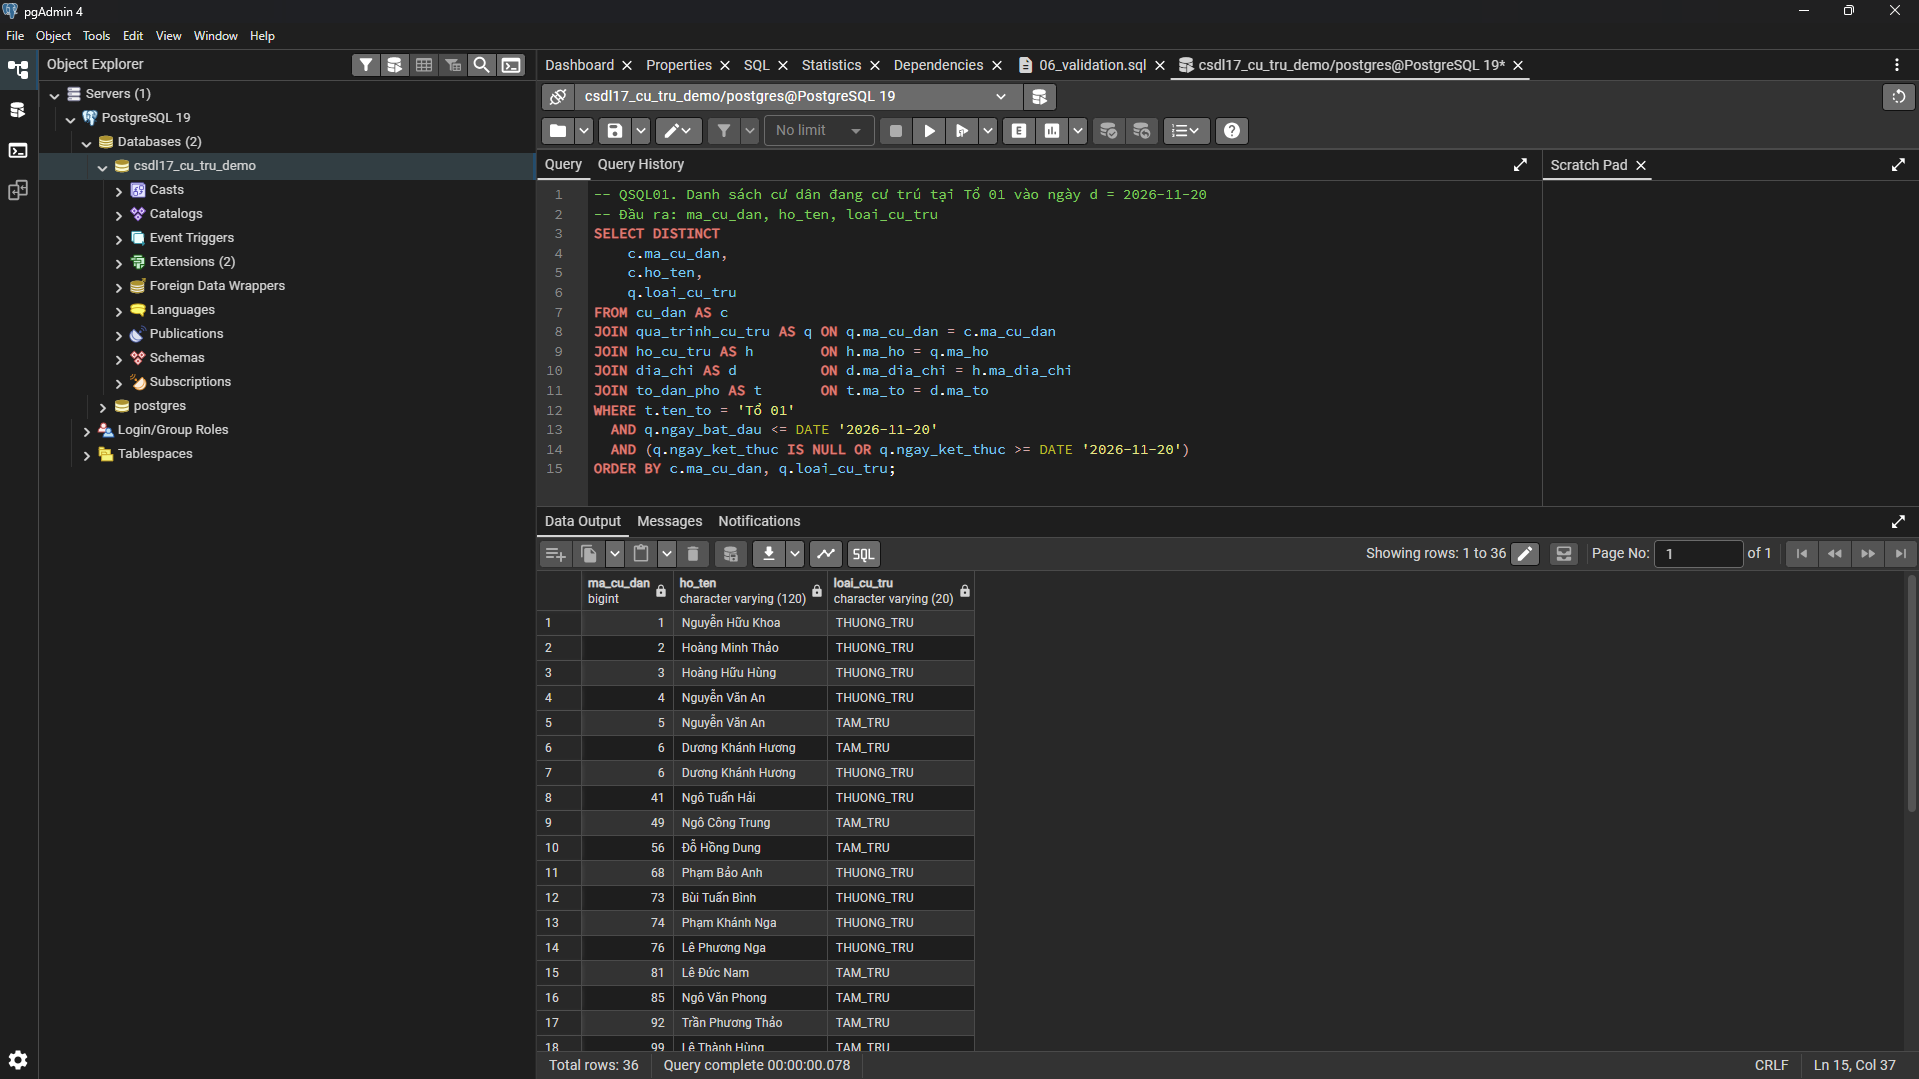
\includegraphics[trim=382bp 0bp 365bp 33bp,clip,width=\linewidth,height=.75\textheight,keepaspectratio]{image/qsql/QSQL01_result.png}
    \caption{QSQL01 --- Cư dân đang cư trú tại Tổ 01}
    \label{fig:qsql01}
\end{figure}
\clearpage

\begin{figure}[H]
    \centering
    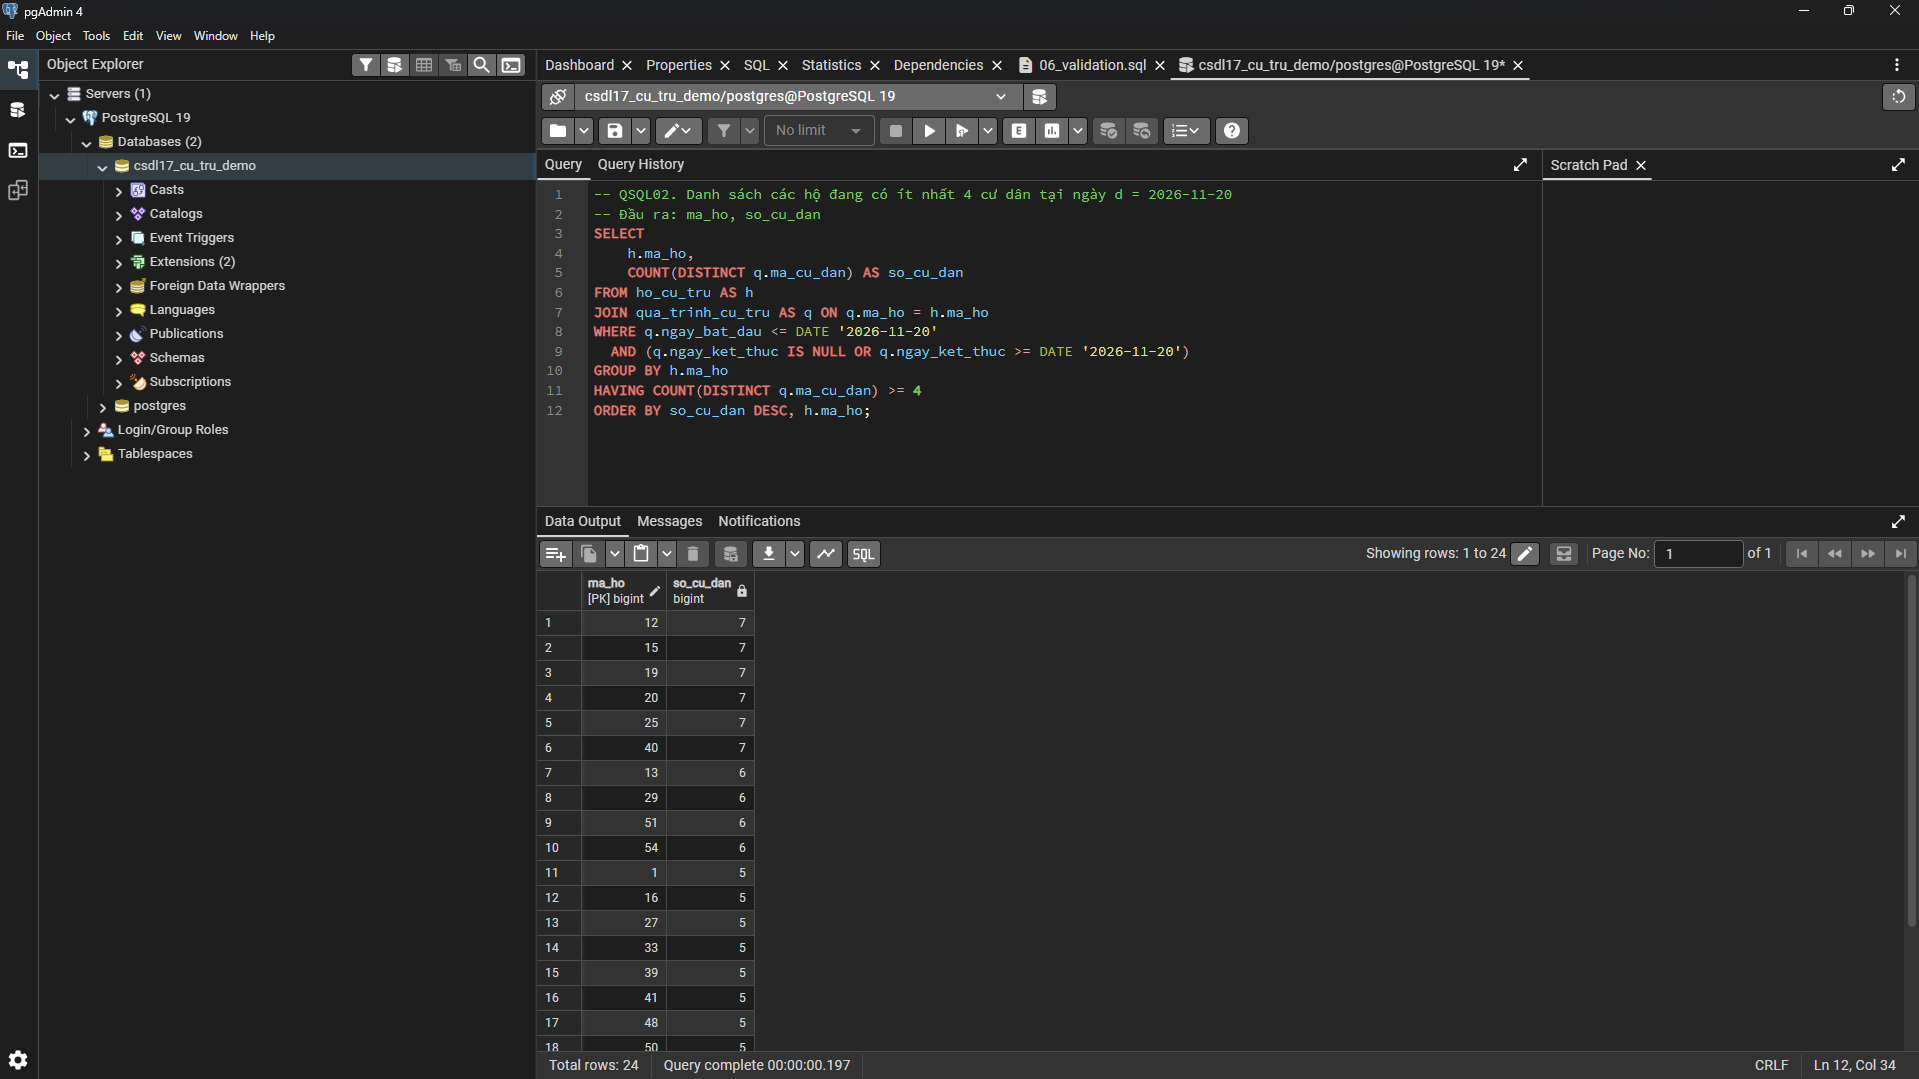
\includegraphics[trim=382bp 0bp 365bp 33bp,clip,width=\linewidth,height=.75\textheight,keepaspectratio]{image/qsql/QSQL02_result.png}
    \caption{QSQL02 --- Hộ có ít nhất 4 cư dân}
    \label{fig:qsql02}
\end{figure}
\clearpage

\begin{figure}[H]
    \centering
    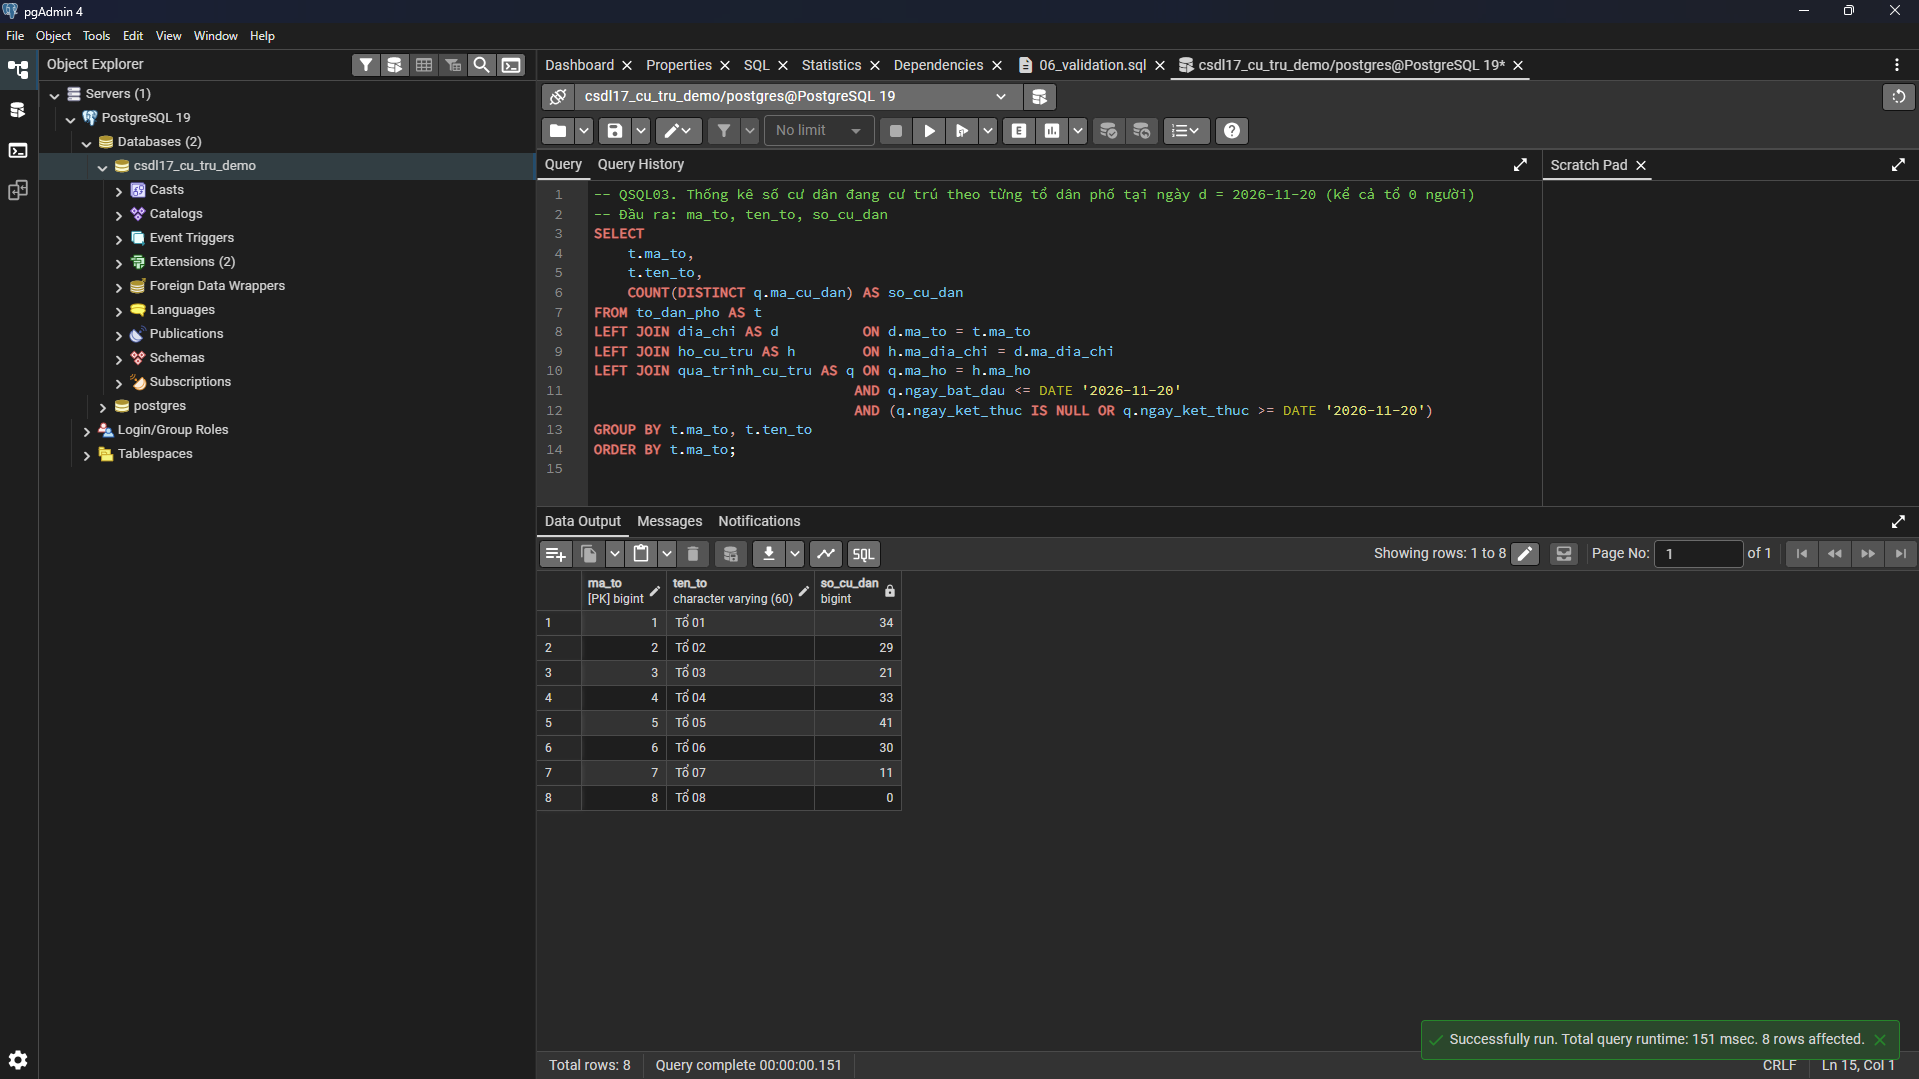
\includegraphics[trim=382bp 0bp 335bp 33bp,clip,width=\linewidth,height=.75\textheight,keepaspectratio]{image/qsql/QSQL03_result.png}
    \caption{QSQL03 --- Thống kê cư dân theo tổ dân phố}
    \label{fig:qsql03}
\end{figure}
\clearpage

\begin{figure}[H]
    \centering
    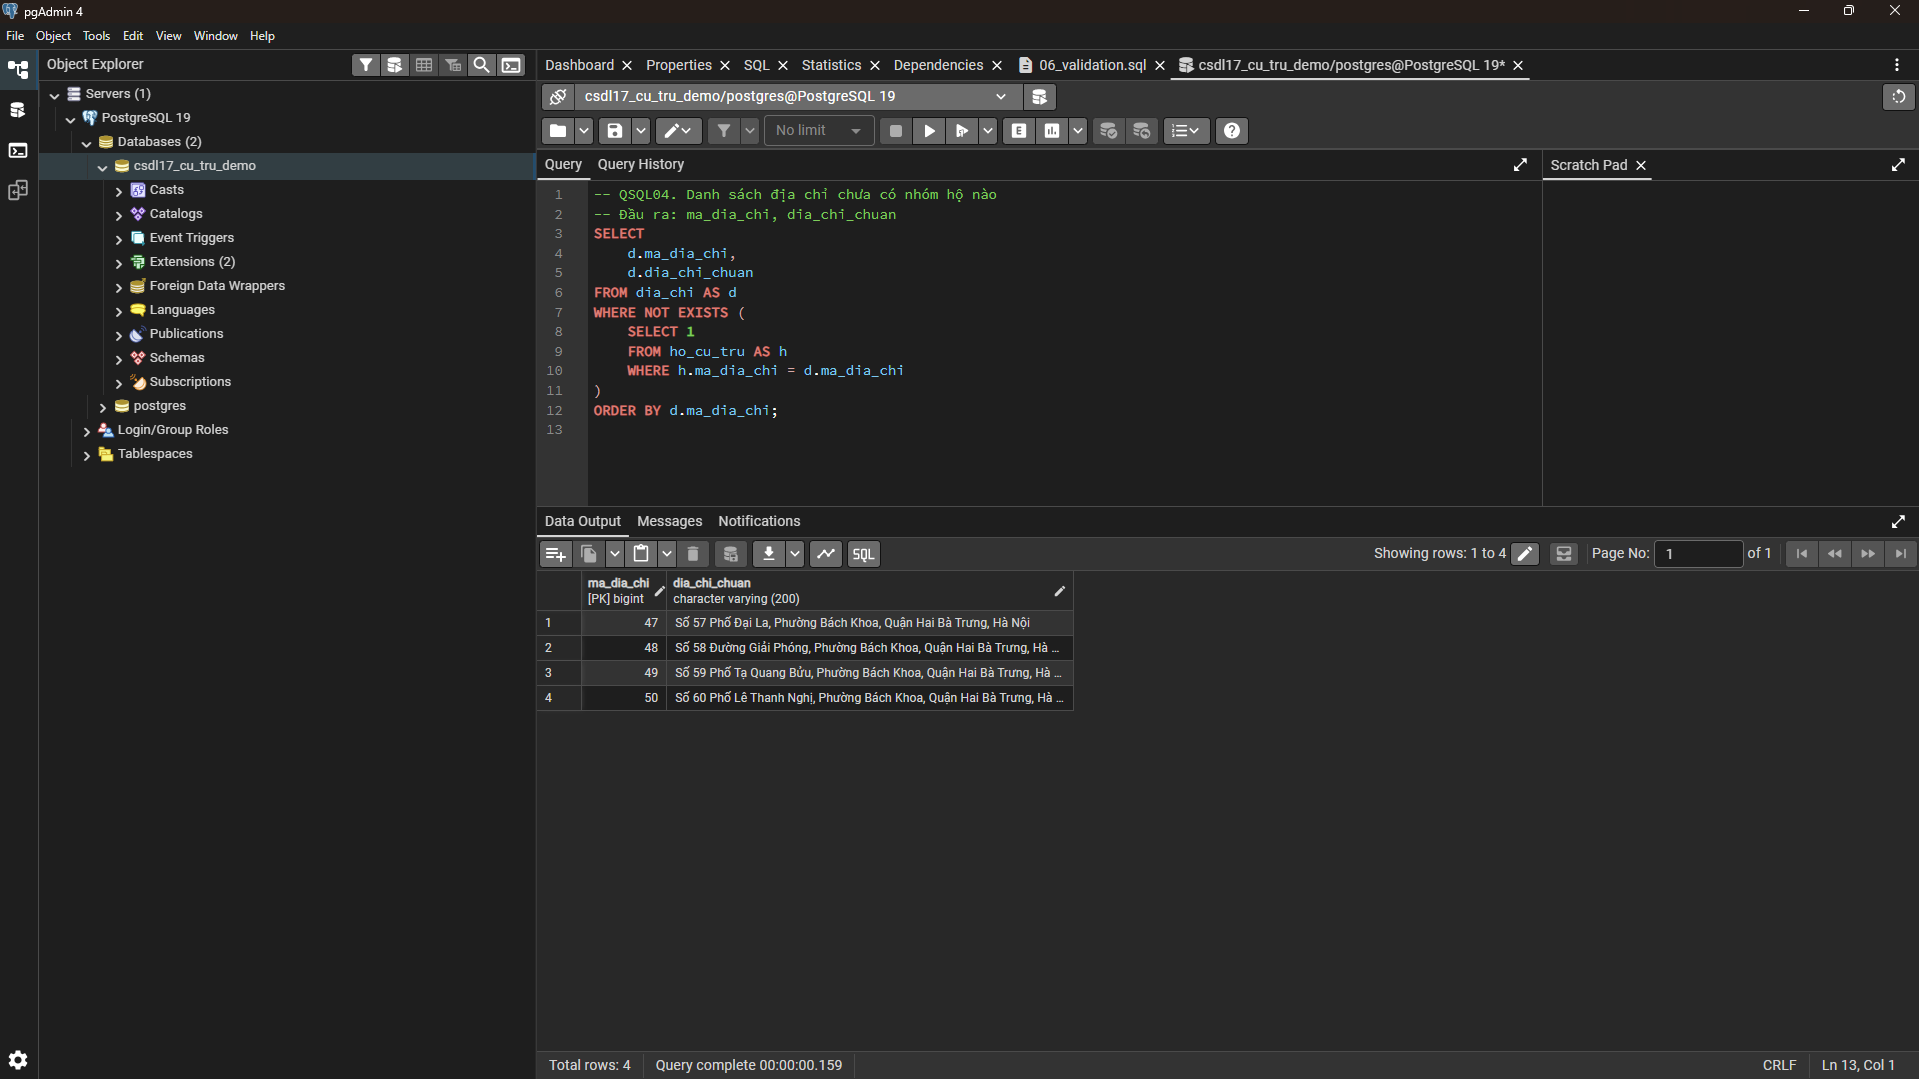
\includegraphics[trim=382bp 0bp 365bp 33bp,clip,width=\linewidth,height=.75\textheight,keepaspectratio]{image/qsql/QSQL04_result.png}
    \caption{QSQL04 --- Địa chỉ chưa có hộ cư trú}
    \label{fig:qsql04}
\end{figure}
\clearpage

\begin{figure}[H]
    \centering
    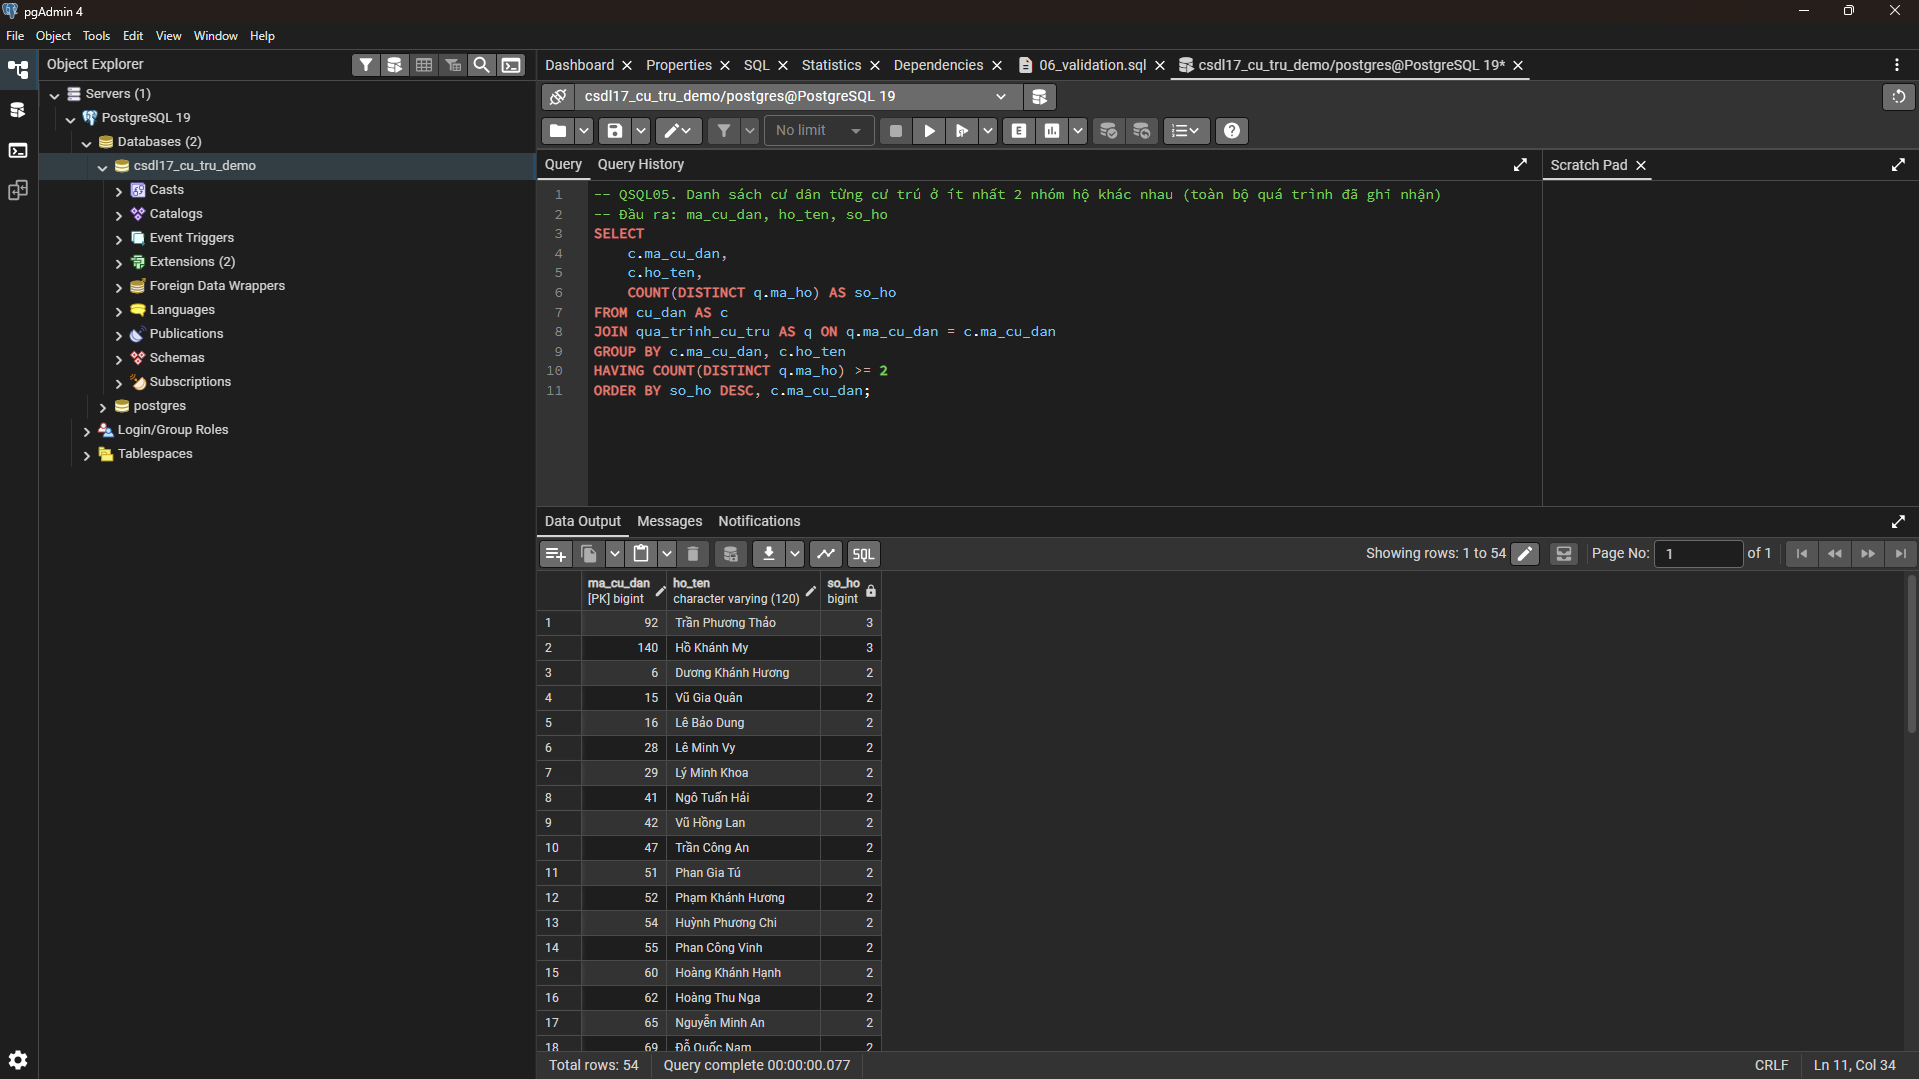
\includegraphics[trim=382bp 0bp 365bp 33bp,clip,width=\linewidth,height=.75\textheight,keepaspectratio]{image/qsql/QSQL05_result.png}
    \caption{QSQL05 --- Cư dân từng ở ít nhất hai hộ}
    \label{fig:qsql05}
\end{figure}
\clearpage

\begin{figure}[H]
    \centering
    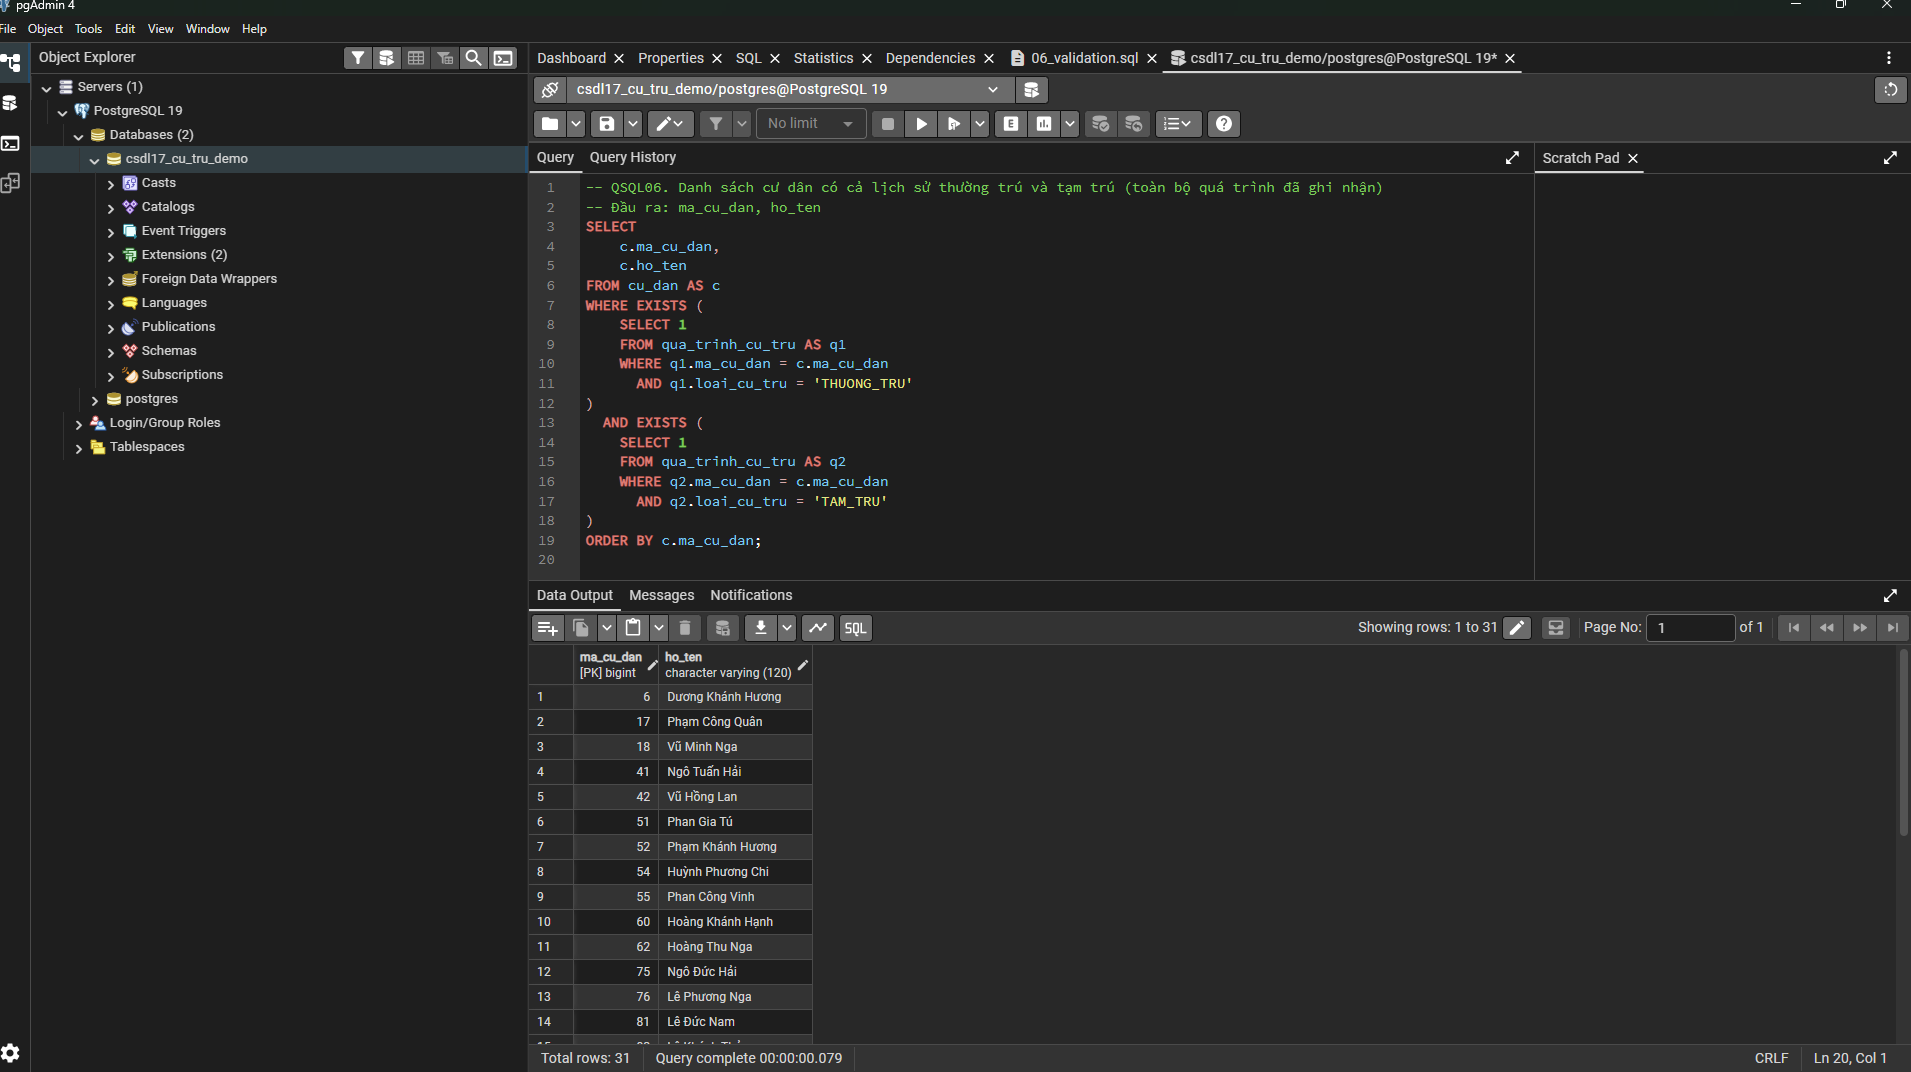
\includegraphics[trim=382bp 0bp 365bp 33bp,clip,width=\linewidth,height=.75\textheight,keepaspectratio]{image/qsql/QSQL06_result.png}
    \caption{QSQL06 --- Cư dân có cả thường trú và tạm trú}
    \label{fig:qsql06}
\end{figure}
\clearpage

\begin{figure}[H]
    \centering
    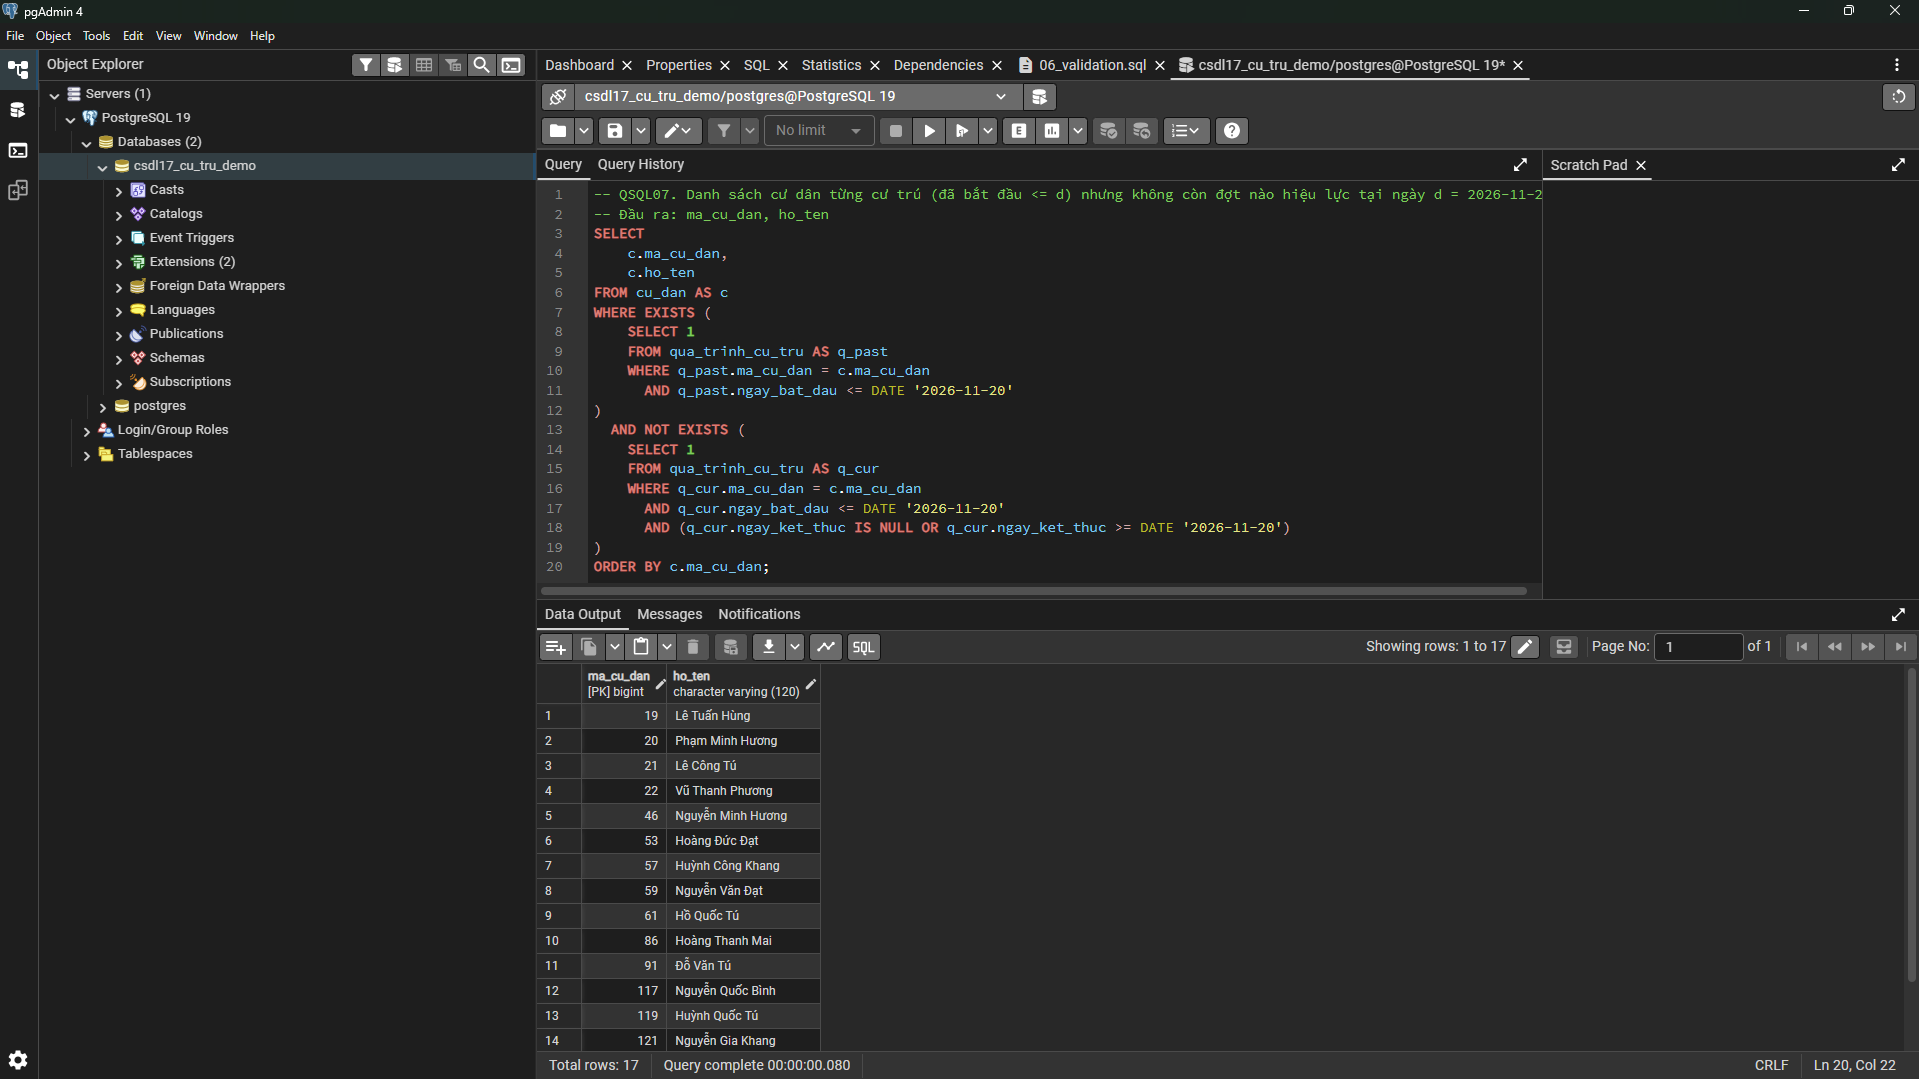
\includegraphics[trim=382bp 0bp 365bp 33bp,clip,width=\linewidth,height=.75\textheight,keepaspectratio]{image/qsql/QSQL07_result.png}
    \caption{QSQL07 --- Cư dân từng ở nhưng đã hết hiệu lực}
    \label{fig:qsql07}
\end{figure}
\clearpage

\begin{figure}[H]
    \centering
    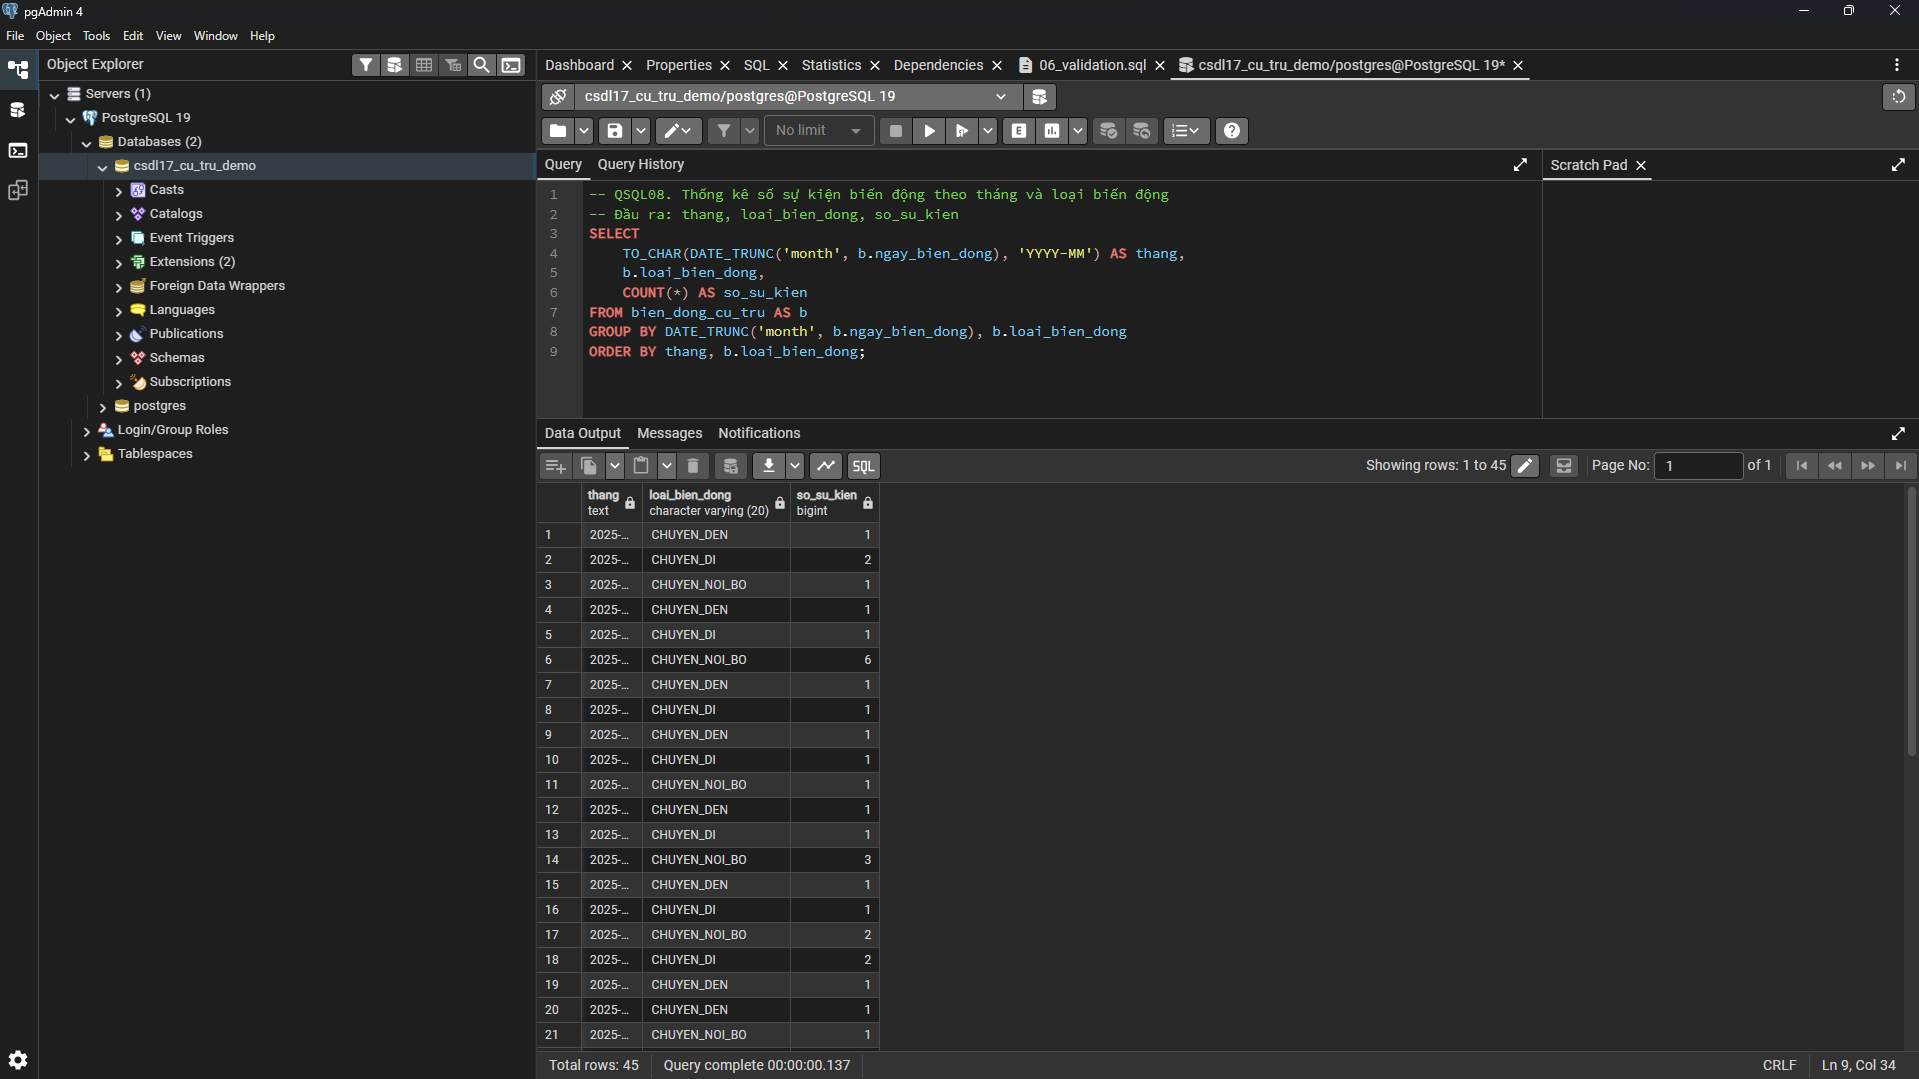
\includegraphics[trim=382bp 0bp 365bp 33bp,clip,width=\linewidth,height=.75\textheight,keepaspectratio]{image/qsql/QSQL08_result.png}
    \caption{QSQL08 --- Thống kê biến động theo tháng và loại}
    \label{fig:qsql08}
\end{figure}
\clearpage

\begin{figure}[H]
    \centering
    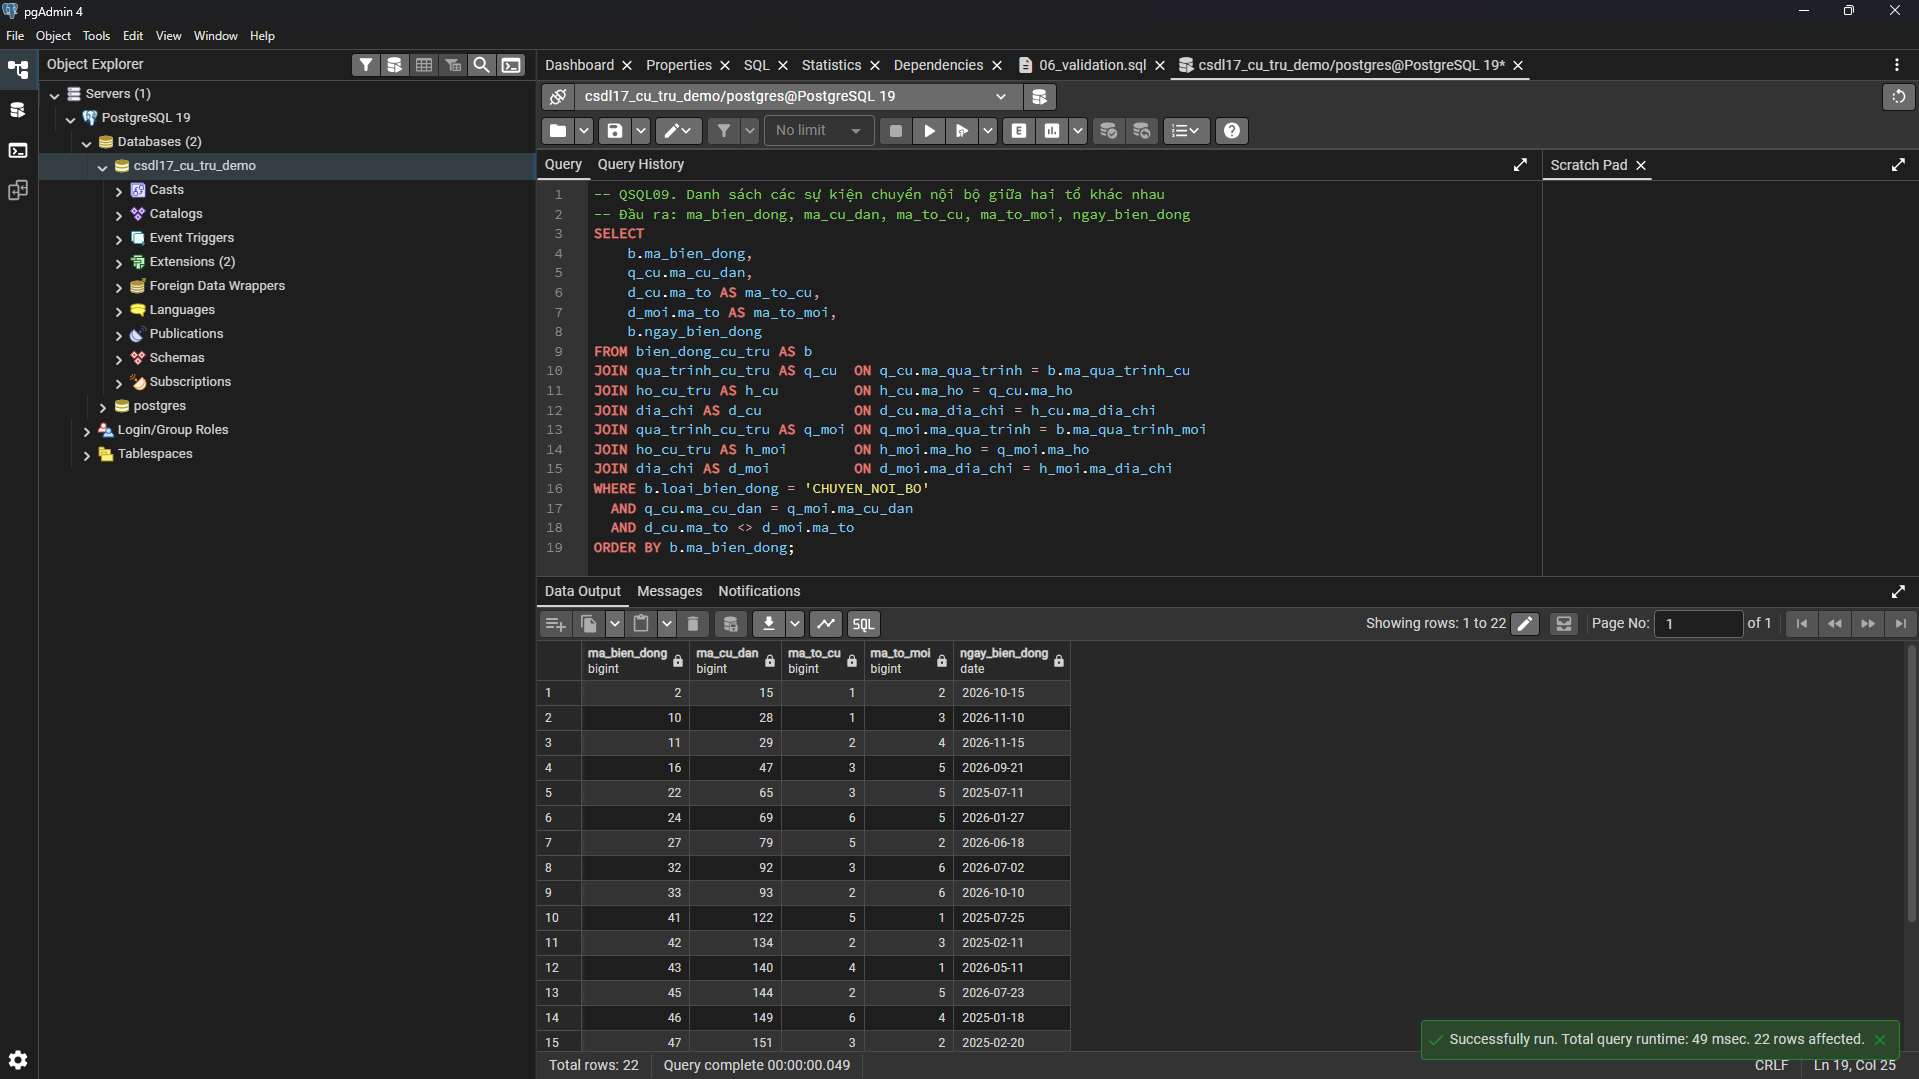
\includegraphics[trim=382bp 0bp 365bp 33bp,clip,width=\linewidth,height=.75\textheight,keepaspectratio]{image/qsql/QSQL09_result.png}
    \caption{QSQL09 --- Chuyển nội bộ giữa hai tổ}
    \label{fig:qsql09}
\end{figure}
\clearpage

\begin{figure}[H]
    \centering
    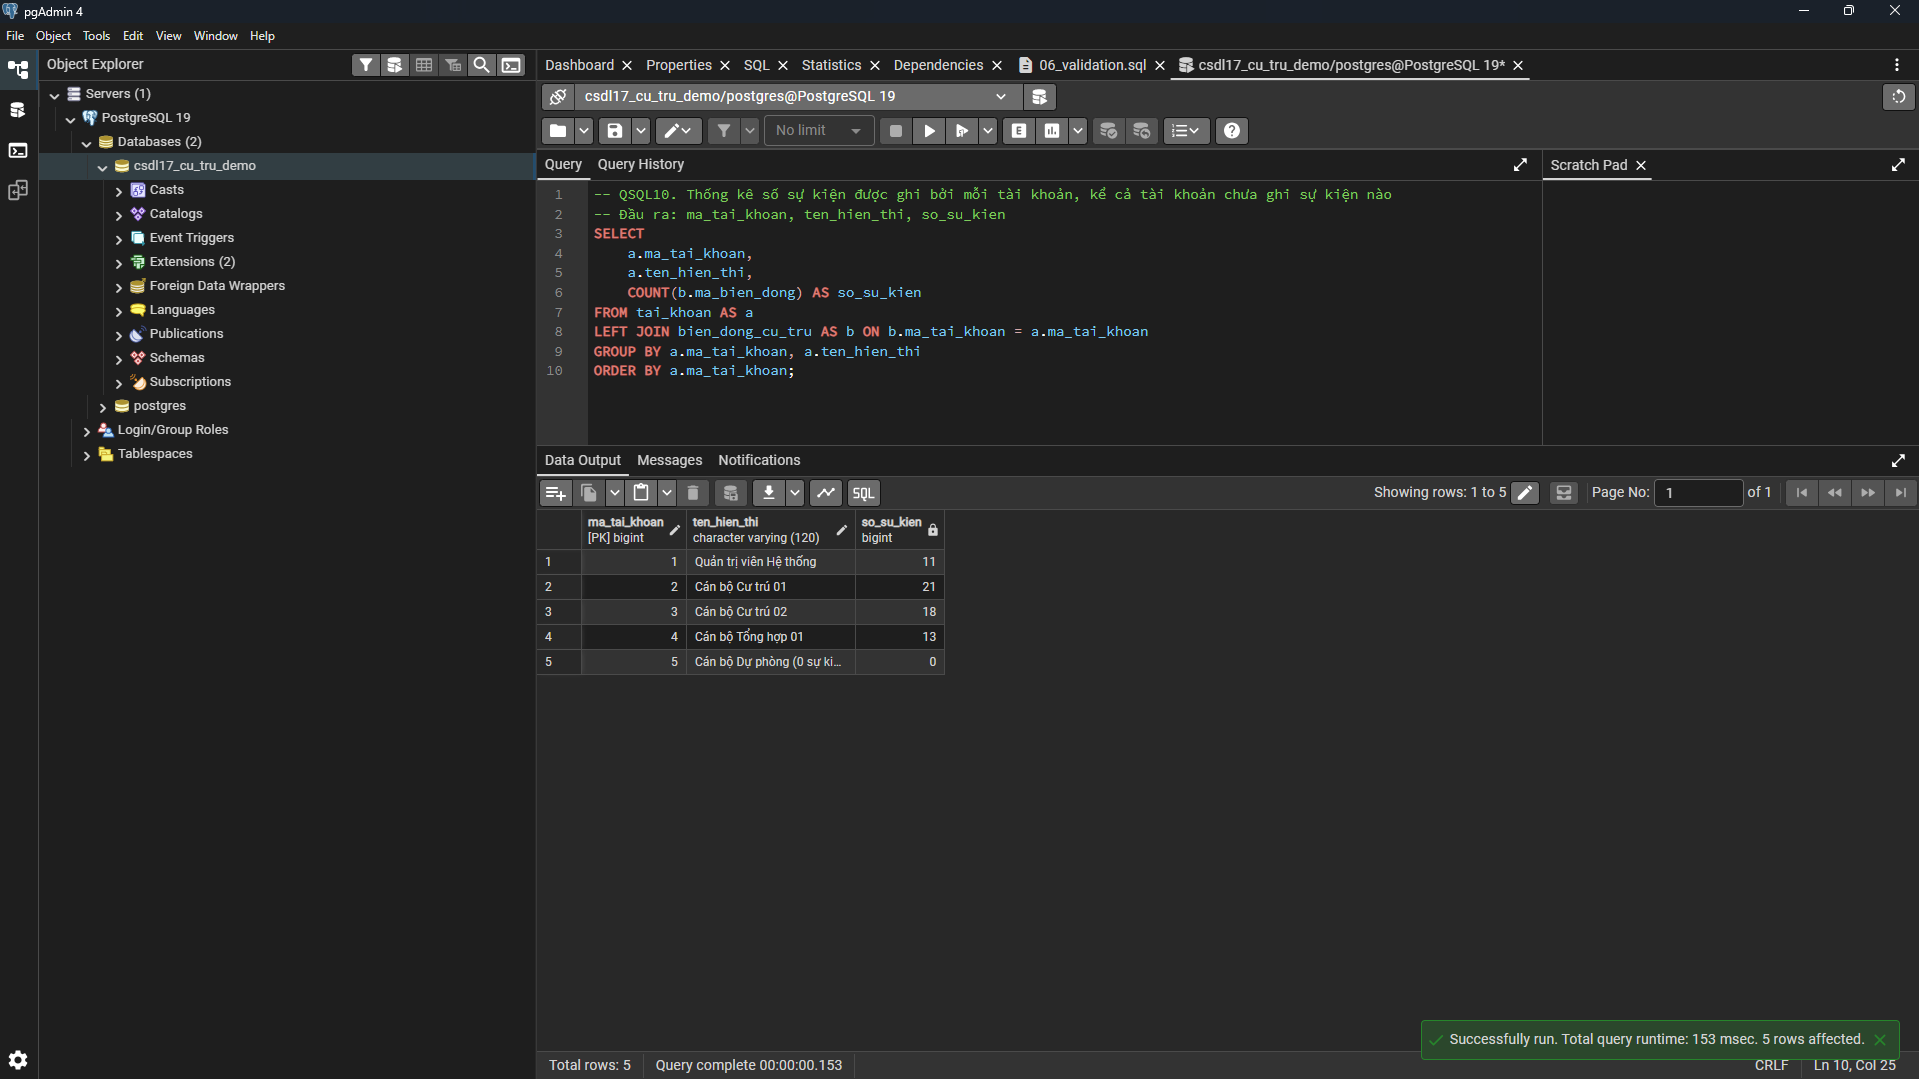
\includegraphics[trim=382bp 0bp 365bp 33bp,clip,width=\linewidth,height=.75\textheight,keepaspectratio]{image/qsql/QSQL10_result.png}
    \caption{QSQL10 --- Số biến động theo tài khoản}
    \label{fig:qsql10}
\end{figure}
\clearpage

\phantomsection
\section*{PHỤ LỤC. ẢNH KIỂM THỬ BẢO MẬT}
\addcontentsline{toc}{section}{PHỤ LỤC. ẢNH KIỂM THỬ BẢO MẬT}
\label{sec:anh-sec}

Ba ảnh bổ trợ làm rõ cấu hình quyền, kết quả kiểm tra bản ghi trước và sau phép thử B1, và định nghĩa VIEW dùng trong B2.

\begin{figure}[H]
    \centering
    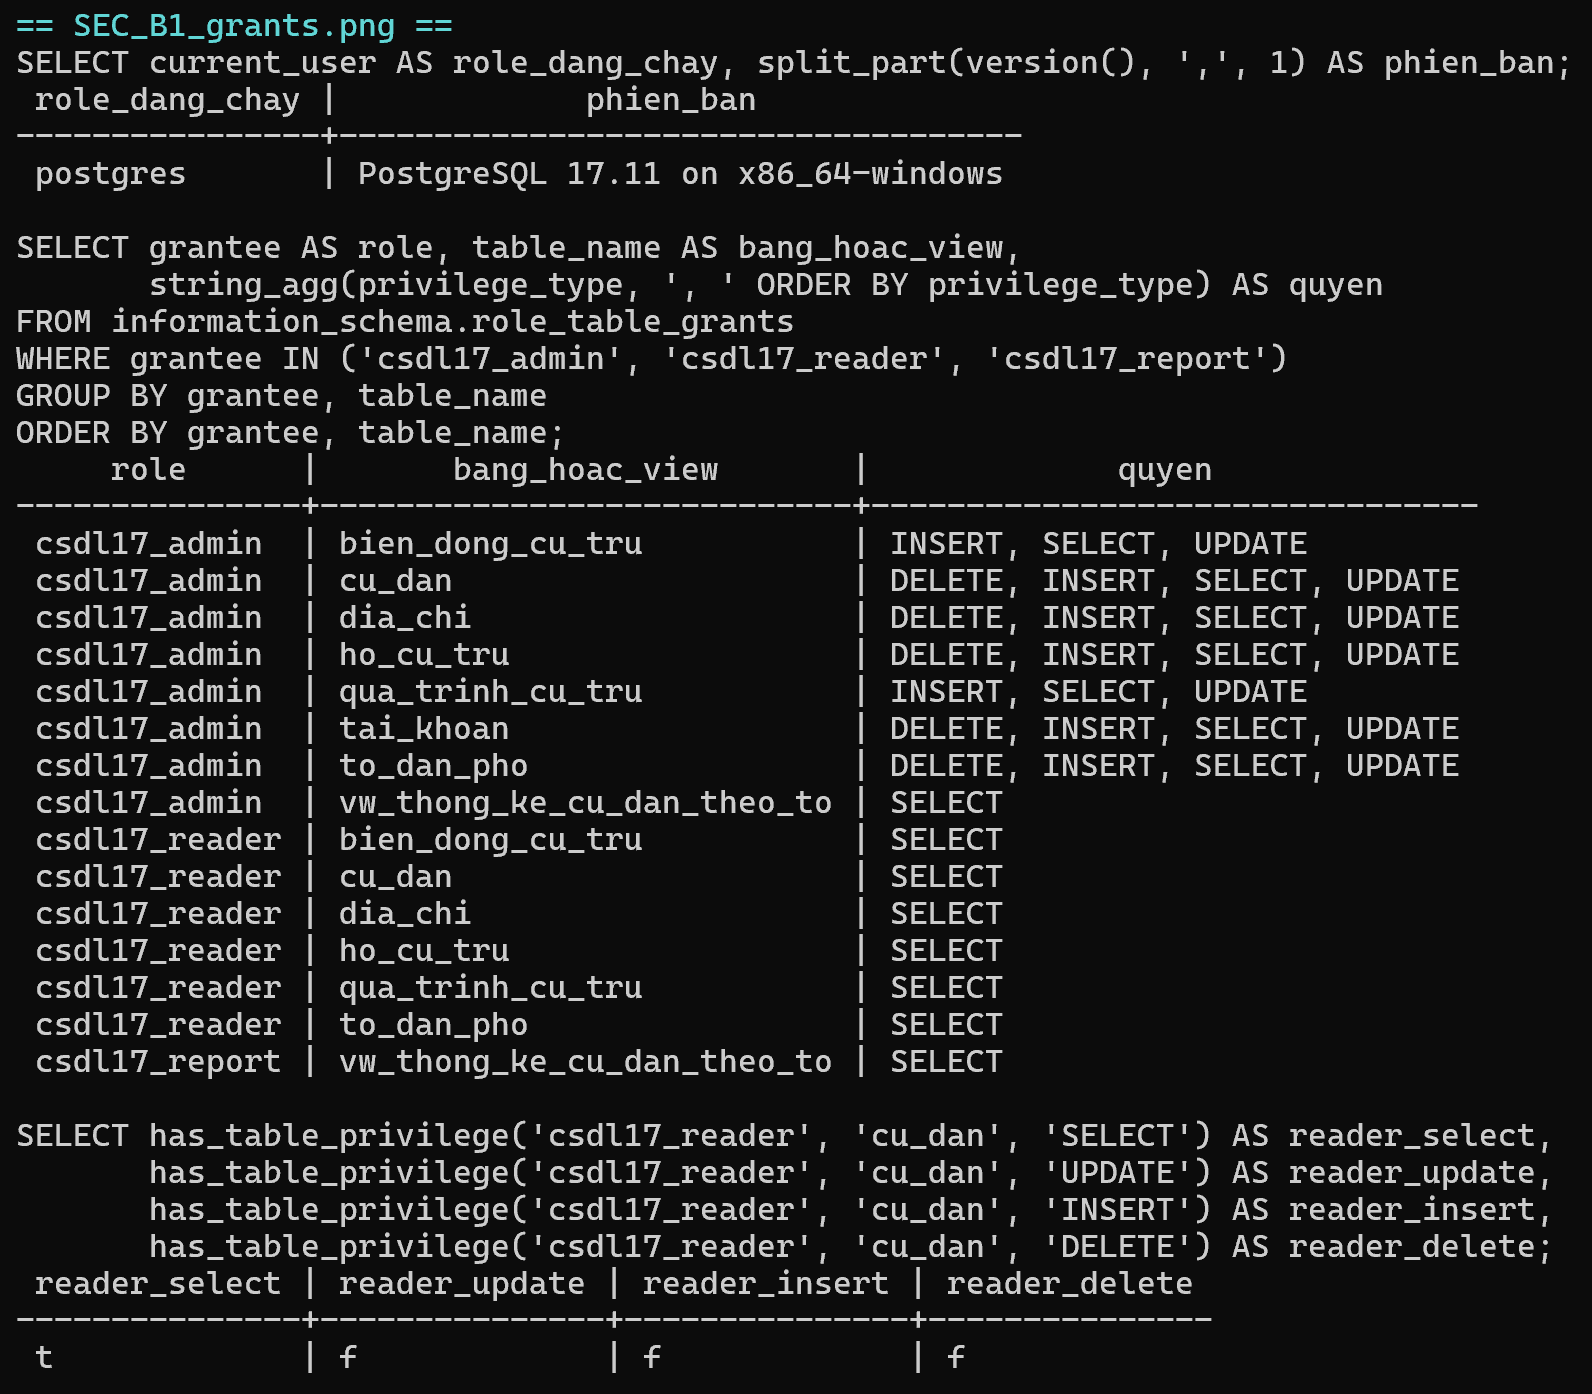
\includegraphics[width=\linewidth,height=.76\textheight,keepaspectratio]{image/security/SEC_B1_grants.png}
    \caption{B1 --- Quyền của ba role trên các bảng và VIEW}
\end{figure}
\clearpage

\begin{figure}[H]
    \centering
    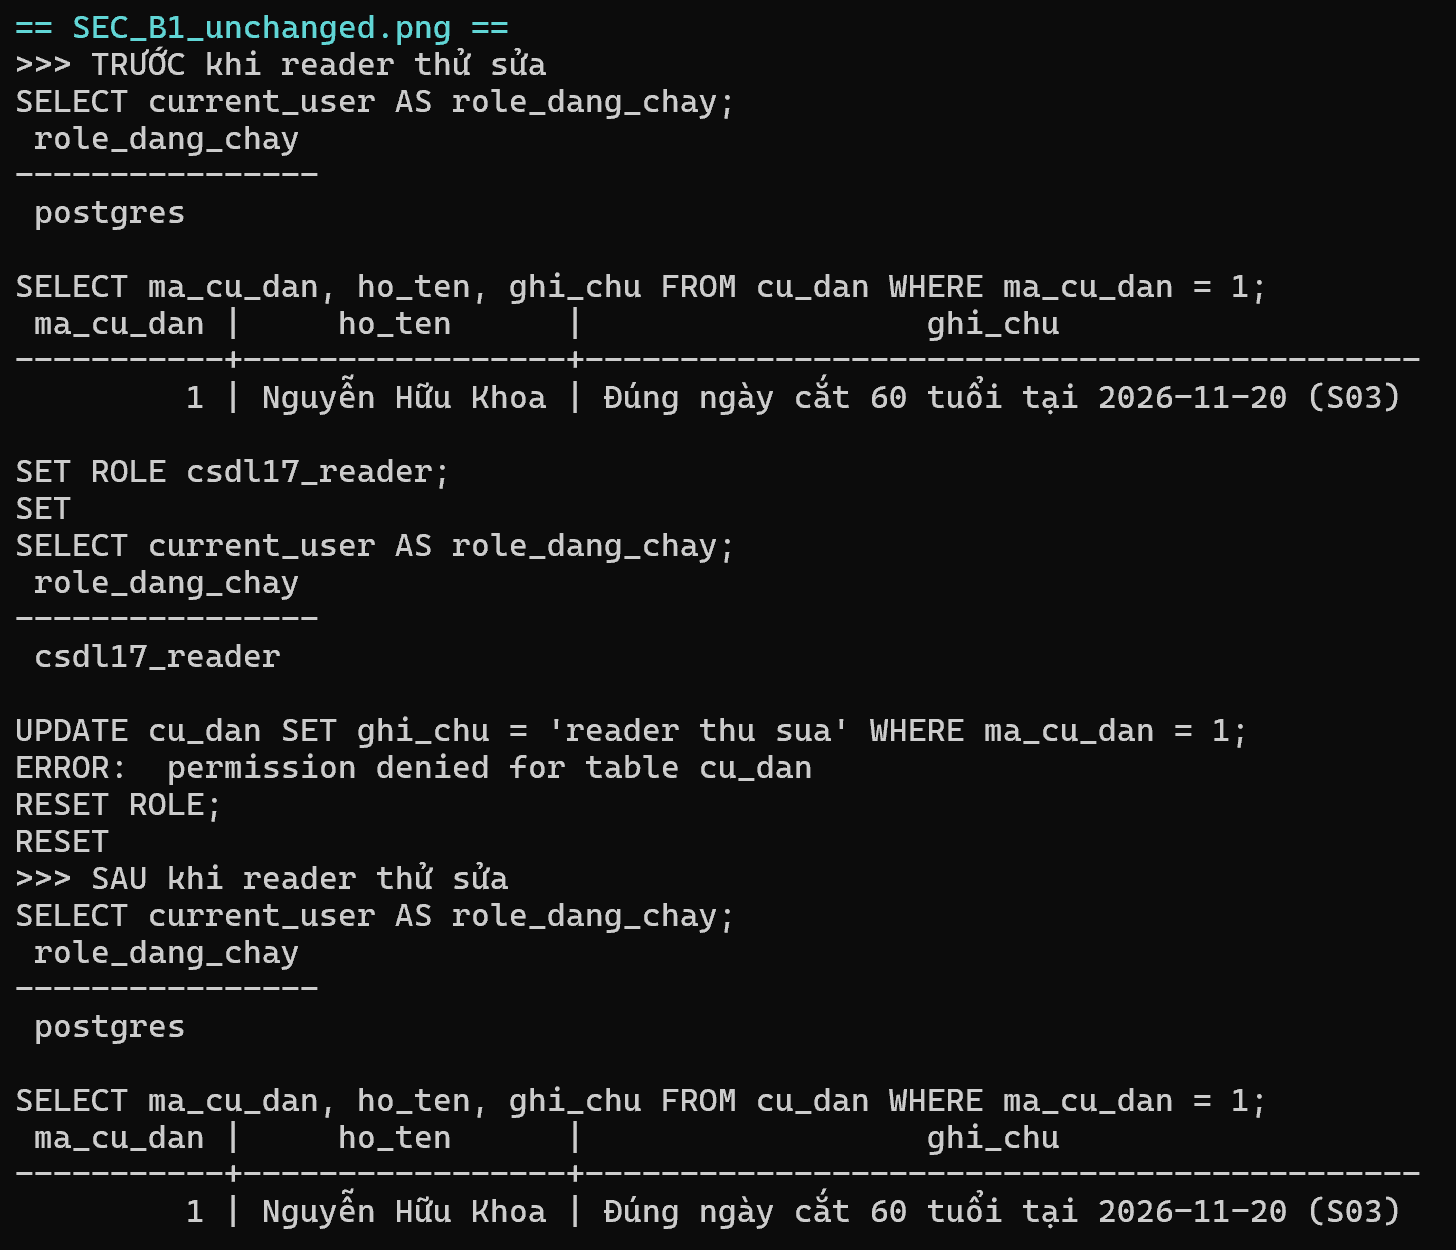
\includegraphics[width=\linewidth,height=.76\textheight,keepaspectratio]{image/security/SEC_B1_unchanged.png}
    \caption{B1 --- Giá trị của bản ghi kiểm tra trước và sau phép thử}
\end{figure}
\clearpage

\begin{figure}[H]
    \centering
    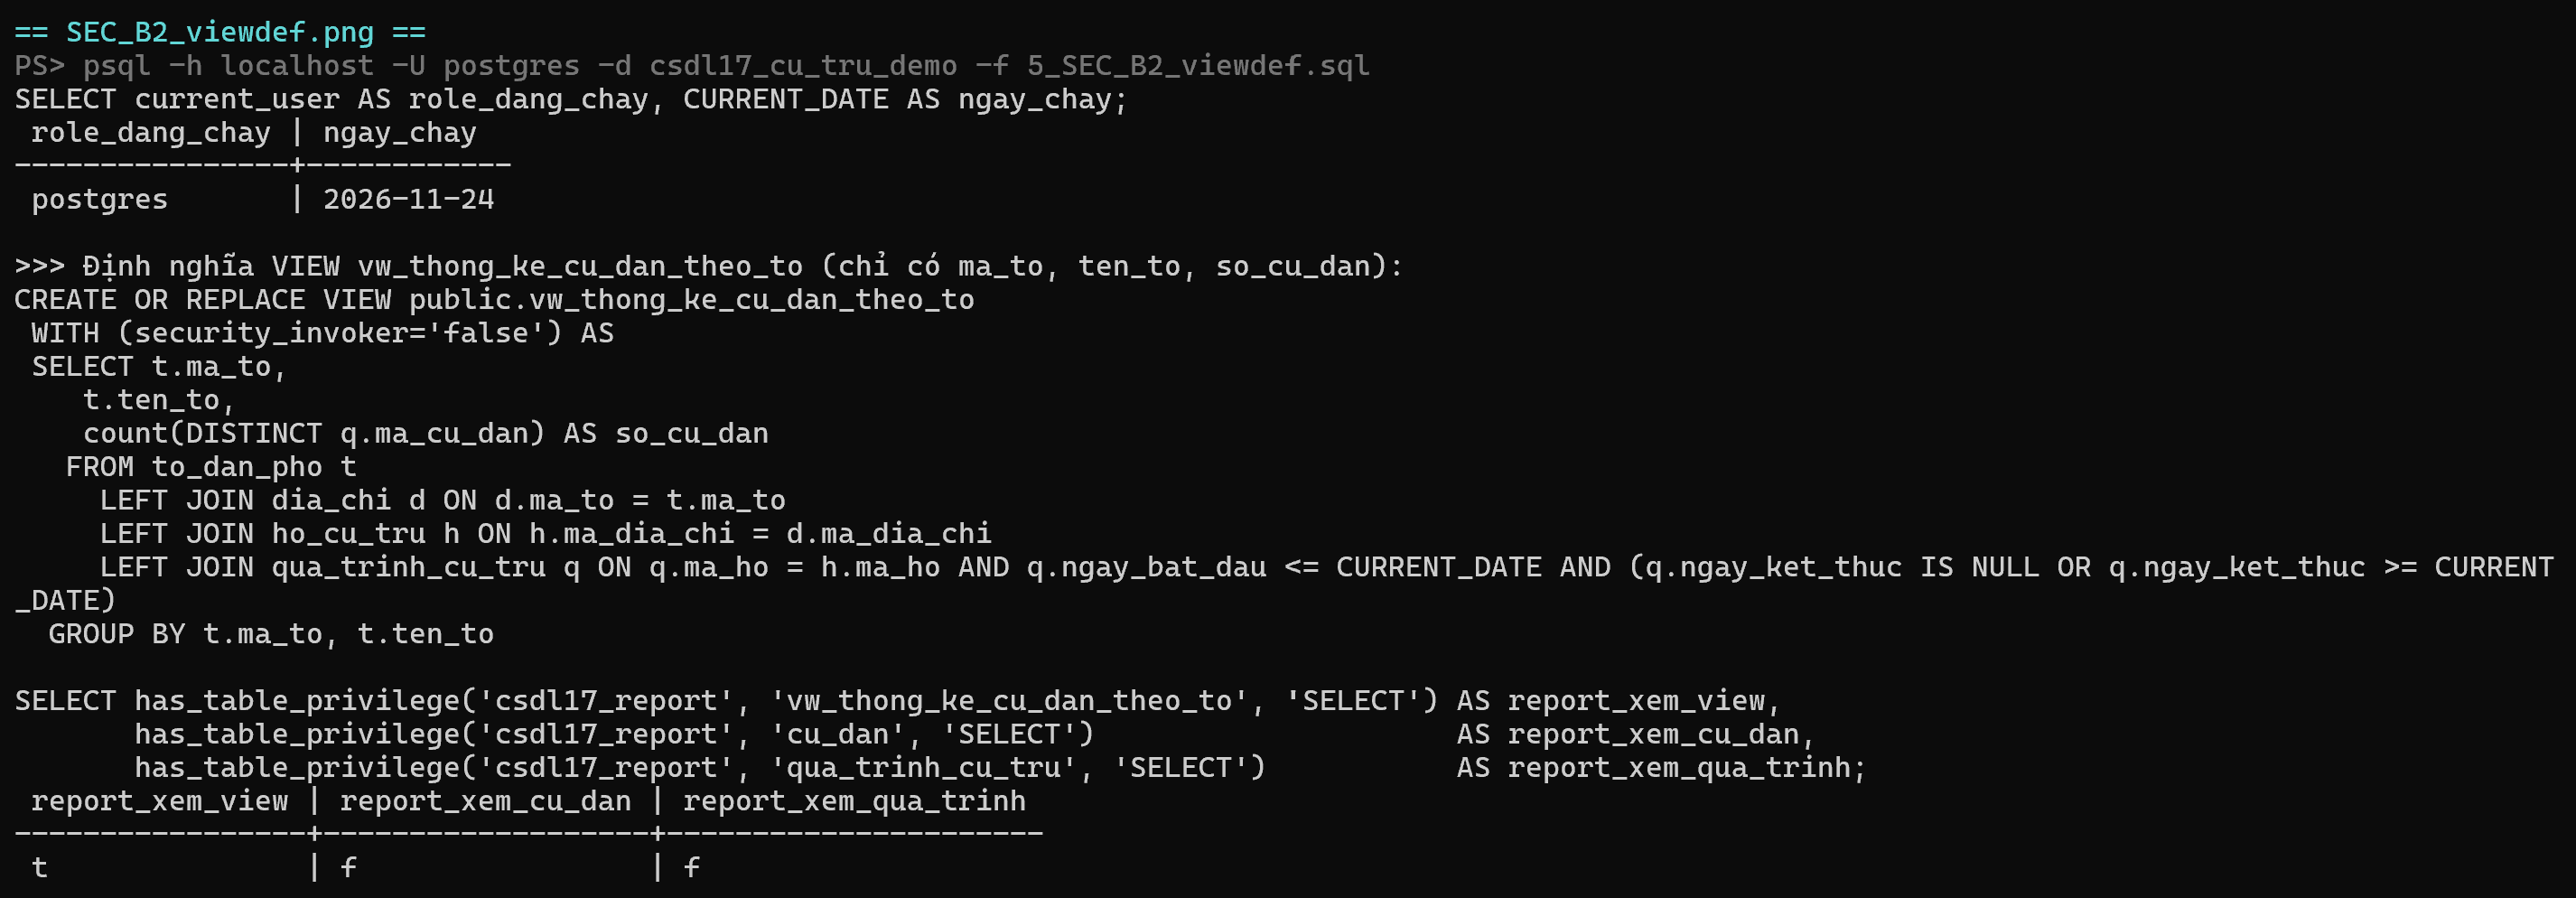
\includegraphics[width=\linewidth]{image/security/SEC_B2_viewdef.png}
    \caption{B2 --- Định nghĩa VIEW trong cơ sở dữ liệu demo và kết quả kiểm tra quyền}
\end{figure}

Ảnh trên được chụp từ bản VIEW thử nghiệm trước đó, dùng \texttt{CURRENT\_DATE} và chạy ngày 24/11/2026. Bản chính thức trong \texttt{sql/05\_security.sql} và ở Chương 6 cố định ngày 20/11/2026. Nhóm đã đếm lại theo cả hai ngày: số cư dân của tám tổ trùng khớp (34, 29, 21, 33, 41, 30, 11 và 0), vì giữa hai ngày này không có đợt cư trú nào bắt đầu hoặc kết thúc làm thay đổi kết quả. Phần kiểm tra quyền không phụ thuộc ngày.
\clearpage

% Trang cuối: phân công công việc và đánh giá đóng góp
\phantomsection
\section*{Bảng phân công công việc}
\addcontentsline{toc}{section}{Bảng phân công công việc}
\vspace{10pt}

Bảng dưới đây ghi phần việc của từng thành viên. Cột xếp loại và chữ ký để nhóm thống nhất đánh giá, điền và ký xác nhận trước khi nộp; thang xếp loại gồm A (đóng góp tốt), B (đóng góp khá), C (đóng góp ít).

\begin{table}[H]
    \centering
    \renewcommand{\arraystretch}{1.35}
    \setlength{\tabcolsep}{5pt}
    \begin{tabularx}{\textwidth}{|>{\RaggedRight\arraybackslash}m{3.3cm}|>{\centering\arraybackslash}m{1.9cm}|Y|>{\centering\arraybackslash}m{1.5cm}|>{\centering\arraybackslash}m{2.3cm}|}
        \hline
        \textbf{Họ và tên} & \textbf{MSSV} & \textbf{Công việc được giao} & \textbf{Xếp loại} & \textbf{Chữ ký} \\
        \hline
        \rule{0pt}{6ex} Trần Bùi Tùng Linh & 20227057 & Nghiệp vụ, thiết kế, ràng buộc, tích hợp & & \\
        \hline
        \rule{0pt}{6ex} Trần Tuấn Ngọc & 20227064 & Dữ liệu, SQL, kiểm thử & & \\
        \hline
        \rule{0pt}{6ex} Dương Ngọc Ninh & 20237469 & Đại số quan hệ, bảo mật, review & & \\
        \hline
    \end{tabularx}
    \label{tab:phancong}
\end{table}


\end{document}
